% SPDX-License-Identifier: CC-BY-4.0
%
% Copyright (c) 2023 Nelson Vieira
%
% @author Nelson Vieira <2080511@student.uma.pt>
% @license CC-BY-4.0 <https://creativecommons.org/licenses/by/4.0/legalcode.txt>
\chapter*[Appendix]{Appendix}

\section*[Appendix A]{Appendix A: Survey}\label{appendix:survey}

\subsection*{Digital literacy related to privacy in Internet of Things}

This survey is being carried out within the scope of the Master's thesis in
Computer Engineering at the University of Madeira, created by Nelson Vieira,
aims to collect information regarding users' knowledge in terms of privacy rights
in the Internet of Things. It is an exploratory work for the design and creation
of tools for training users in terms of privacy issues.

To this end, we ask for your cooperation in collecting this information and
responding as honestly and sincerely as possible. Even if some answers may
seem wrong to you please respond with the answer that best fits your view/understanding,
there are no wrong answers. Being guaranteed that all participants will be kept
anonymous, no data will be used for purposes other than those established within
the scope of this thesis, and will not be used to in any way identify anyone.

This survey is open to anyone that is 18 years or older.

Participation is entirely voluntary. You should only participate if you want
to, and not participating will have no negative consequences. If you choose
not to engage in this study, it will have no effect on your rights. You may
still withdraw at any moment and for any reason. This would have no effect
on your legal rights.

Completing the  survey takes an average of 15 to 20 minutes. We thank you in
advance for your collaboration.

If you want to follow the work or have any specific questions, you can contact
Nelson Vieira through the following email: literaciadigitaliot@gmail.com

P.S.: This survey contains credits to get free survey responses at SurveySwap.io

\vspace{0.3cm}
0. I am aware of the terms described above.

\vspace{0.6cm}
\begin{center}
    \noindent\begin{tabularx}{0.8\textwidth}{ >{\centering\arraybackslash}X >{\raggedright\arraybackslash}X }
        {\huge $\circ$} & Yes, I agree that my data will be processed as described \\[0.2cm]
        {\huge $\circ$} & I do not want to participate in this questionnaire
    \end{tabularx}
\end{center}
\vspace{0.6cm}

\subsection*{Section 1: General knowledge and attitudes towards privacy}

The purpose of this section is to ask general questions about your knowledge
in the area of information privacy.

1. ``Privacy is important to me''. Do you agree with this statement?

\vspace{0.6cm}
\begin{center}
    \noindent\begin{tabularx}{0.8\textwidth}{ >{\centering\arraybackslash}X >{\centering\arraybackslash}X >{\centering\arraybackslash}X >{\centering\arraybackslash}X >{\centering\arraybackslash}X >{\centering\arraybackslash}X >{\centering\arraybackslash}X >{\centering\arraybackslash}X >{\centering\arraybackslash}X }
        & 1 & 2 & 3 & 4 & 5 & 6 & 7 & \\[0.2cm]
        Disagree & {\huge $\circ$} & {\huge $\circ$} & {\huge $\circ$} & {\huge $\circ$} & {\huge $\circ$} & {\huge $\circ$} & {\huge $\circ$} & Agree
    \end{tabularx}
\end{center}
\vspace{0.6cm}

2. ``I know techniques to guarantee privacy and the protection of my data when I use the Internet''. Do you agree with this statement?

\vspace{0.6cm}
\begin{center}
    \noindent\begin{tabularx}{0.8\textwidth}{ >{\centering\arraybackslash}X >{\centering\arraybackslash}X >{\centering\arraybackslash}X >{\centering\arraybackslash}X >{\centering\arraybackslash}X >{\centering\arraybackslash}X >{\centering\arraybackslash}X >{\centering\arraybackslash}X >{\centering\arraybackslash}X }
        & 1 & 2 & 3 & 4 & 5 & 6 & 7 & \\[0.2cm]
        Disagree & {\huge $\circ$} & {\huge $\circ$} & {\huge $\circ$} & {\huge $\circ$} & {\huge $\circ$} & {\huge $\circ$} & {\huge $\circ$} & Agree
    \end{tabularx}
\end{center}
\vspace{0.6cm}

3. Could you give examples of techniques or strategies you use to guarantee the privacy and protection of your data?

\vspace{0.6cm}
\begin{center}
    \noindent\begin{tabularx}{0.9\textwidth}{ |>{\raggedright\arraybackslash}X| }
        \hline
        \hspace{0.2cm}Short answer...\vspace{0.5cm} \\
        \hline
    \end{tabularx}
\end{center}
\vspace{0.6cm}

4. Do you think your data privacy is important?

\vspace{0.6cm}
\begin{center}
    \noindent\begin{tabular}{ p{2cm} p{1.3cm} p{1.3cm} p{1.3cm} p{1.3cm} p{1.3cm} p{1.3cm} p{1.3cm} p{2.5cm} }
        & \centering 1 & \centering 2 & \centering 3 & \centering 4 & \centering 5 & \centering 6 & \centering 7 & \\[0.2cm]
        Not at all & \centering {\huge $\circ$} & \centering {\huge $\circ$} & \centering {\huge $\circ$} & \centering {\huge $\circ$} & \centering {\huge $\circ$} & \centering {\huge $\circ$} & \centering {\huge $\circ$} & Very important
    \end{tabular}
\end{center}
\vspace{0.6cm}

5. How do you define data (or digital) privacy?

\vspace{0.6cm}
\begin{center}
    \noindent\begin{tabularx}{0.9\textwidth}{ |>{\raggedright\arraybackslash}X| }
        \hline
        \hspace{0.2cm}Long answer...\vspace{1.75cm} \\
        \hline
    \end{tabularx}
\end{center}
\vspace{0.6cm}

6. Do you think your data privacy is relevant nowadays?

\vspace{0.6cm}
\begin{center}
    \noindent\begin{tabular}{ p{2cm} p{1.3cm} p{1.3cm} p{1.3cm} p{1.3cm} p{1.3cm} p{1.3cm} p{1.3cm} p{2.5cm} }
        & \centering 1 & \centering 2 & \centering 3 & \centering 4 & \centering 5 & \centering 6 & \centering 7 & \\[0.2cm]
        Not at all & \centering {\huge $\circ$} & \centering {\huge $\circ$} & \centering {\huge $\circ$} & \centering {\huge $\circ$} & \centering {\huge $\circ$} & \centering {\huge $\circ$} & \centering {\huge $\circ$} & Very relevant
    \end{tabular}
\end{center}
\vspace{0.6cm}

7. ``Data privacy is a human right''. Do you agree with this statement?

\vspace{0.6cm}
\begin{center}
    \noindent\begin{tabularx}{0.8\textwidth}{ >{\centering\arraybackslash}X >{\raggedright\arraybackslash}X }
        {\huge $\circ$} & I agree \\[0.2cm]
        {\huge $\circ$} & I disagree \\[0.2cm]
        {\huge $\circ$} & I do not know
    \end{tabularx}
\end{center}
\vspace{0.6cm}

8. ``Data privacy is a consumer right''. Do you agree with this statement?

\vspace{0.6cm}
\begin{center}
    \noindent\begin{tabularx}{0.8\textwidth}{ >{\centering\arraybackslash}X >{\raggedright\arraybackslash}X }
        {\huge $\circ$} & I agree \\[0.2cm]
        {\huge $\circ$} & I disagree \\[0.2cm]
        {\huge $\circ$} & I do not know
    \end{tabularx}
\end{center}
\vspace{0.6cm}

9. In your opinion, are security and privacy synonymous?

\vspace{0.6cm}
\begin{center}
    \noindent\begin{tabularx}{0.8\textwidth}{ >{\centering\arraybackslash}X >{\raggedright\arraybackslash}X }
        {\huge $\circ$} & Yes \\[0.2cm]
        {\huge $\circ$} & No
    \end{tabularx}
\end{center}
\vspace{0.6cm}

10. How familiar are you with the following terms?

\vspace{0.6cm}
\begin{center}
    \noindent\begin{tabular}{ p{4.5cm} p{3cm} p{4cm} p{3cm} }
        & I Know well & I have some knowledge & I do not know \\[0.4cm]
        Cookie & {\huge $\circ$} & {\huge $\circ$} & {\huge $\circ$} \\[0.2cm]
        Wireless networks & {\huge $\circ$} & {\huge $\circ$} & {\huge $\circ$} \\[0.2cm]
        Wi-Fi & {\huge $\circ$} & {\huge $\circ$} & {\huge $\circ$} \\[0.2cm]
        Internet of Things & {\huge $\circ$} & {\huge $\circ$} & {\huge $\circ$} \\[0.2cm]
        Data protection & {\huge $\circ$} & {\huge $\circ$} & {\huge $\circ$} \\[0.2cm]
        Ad hoc network (wireless) & {\huge $\circ$} & {\huge $\circ$} & {\huge $\circ$} \\[0.2cm]
        Ubiquitous computing & {\huge $\circ$} & {\huge $\circ$} & {\huge $\circ$} \\[0.2cm]
        Privacy assistant & {\huge $\circ$} & {\huge $\circ$} & {\huge $\circ$} \\[0.2cm]
        Blockchain & {\huge $\circ$} & {\huge $\circ$} & {\huge $\circ$} \\[0.2cm]
        Differential privacy & {\huge $\circ$} & {\huge $\circ$} & {\huge $\circ$}
    \end{tabular}
\end{center}
\vspace{0.6cm}

11. Do you think your data is stored/collected when you use the internet?

\vspace{0.6cm}
\begin{center}
    \noindent\begin{tabularx}{0.8\textwidth}{ >{\centering\arraybackslash}X >{\raggedright\arraybackslash}X }
        {\huge $\circ$} & Yes \\[0.2cm]
        {\huge $\circ$} & No \\[0.2cm]
        {\huge $\circ$} & I do not know
    \end{tabularx}
\end{center}
\vspace{0.6cm}

12. What means do you think are used to collect your data?

\vspace{0.6cm}
\begin{center}
    \begin{tabular}{r *{4}{ p{6cm} }}
        {\Large $\square$}\hspace{1cm} & Sound (microphones, recorders, etc.) \\[0.2cm]
        {\Large $\square$}\hspace{1cm} & Image (webcams, scanners, etc.) \\[0.2cm]
        {\Large $\square$}\hspace{1cm} & Online Surveys / Questionnaires \\[0.2cm]
        {\Large $\square$}\hspace{1cm} & Hackers (illegal means) \\[0.2cm]
        {\Large $\square$}\hspace{1cm} & Cookies \\[0.2cm]
        {\Large $\square$}\hspace{1cm} & None \\[0.2cm]
        \hhline{~|-|>{\arrayrulecolor{black}}-|>{\arrayrulecolor{black}}-|}
        {\Large $\square$}\hspace{1cm} & \multicolumn{1}{!{\color{black}\vline}c!{\color{black}\vline}}{Another option...} \\ \cline{2-3}
    \end{tabular}
\end{center}
\vspace{0.6cm}

13. What kind of information can be extracted using the collected data?

\vspace{0.6cm}
\begin{center}
    \begin{tabular}{r *{4}{ p{6cm} }}
        {\Large $\square$}\hspace{1cm} & Visited websites information \\[0.2cm]
        {\Large $\square$}\hspace{1cm} & Work productivity \\[0.2cm]
        {\Large $\square$}\hspace{1cm} & Georeferencing data \\[0.2cm]
        {\Large $\square$}\hspace{1cm} & Online habits \\[0.2cm]
        {\Large $\square$}\hspace{1cm} & Online shoppping \\[0.2cm]
        \hhline{~|-|>{\arrayrulecolor{black}}-|>{\arrayrulecolor{black}}-|}
        {\Large $\square$}\hspace{1cm} & \multicolumn{1}{!{\color{black}\vline}c!{\color{black}\vline}}{Another option...} \\ \cline{2-3}
    \end{tabular}
\end{center}
\vspace{0.6cm}

14. For what purposes can organizations use your data?

\vspace{0.6cm}
\begin{center}
    \begin{tabular}{r *{4}{ p{6cm} }}
        {\Large $\square$}\hspace{1cm} & Improve internet usage \\[0.2cm]
        {\Large $\square$}\hspace{1cm} & Costumer profile \\[0.2cm]
        {\Large $\square$}\hspace{1cm} & Targeted advertising \\[0.2cm]
        {\Large $\square$}\hspace{1cm} & Advertising adapted to the nearest locations \\[0.2cm]
        {\Large $\square$}\hspace{1cm} & Selling data to third parties \\[0.2cm]
        \hhline{~|-|>{\arrayrulecolor{black}}-|>{\arrayrulecolor{black}}-|}
        {\Large $\square$}\hspace{1cm} & \multicolumn{1}{!{\color{black}\vline}c!{\color{black}\vline}}{Another option...} \\ \cline{2-3}
    \end{tabular}
\end{center}
\vspace{0.6cm}

15. Which organizations do you consider to have the best privacy behaviour?

\vspace{0.6cm}
\begin{center}
    \begin{tabular}{r *{4}{ p{6cm} }}
        {\Large $\square$}\hspace{1cm} & Amazon \\[0.2cm]
        {\Large $\square$}\hspace{1cm} & Apple \\[0.2cm]
        {\Large $\square$}\hspace{1cm} & Google \\[0.2cm]
        {\Large $\square$}\hspace{1cm} & Meta (Facebook, Whatsapp, Instagram) \\[0.2cm]
        {\Large $\square$}\hspace{1cm} & Microsoft \\[0.2cm]
        {\Large $\square$}\hspace{1cm} & Samsung \\[0.2cm]
        {\Large $\square$}\hspace{1cm} & IBM \\[0.2cm]
        {\Large $\square$}\hspace{1cm} & ScienceSoft \\[0.2cm]
        {\Large $\square$}\hspace{1cm} & PTC \\[0.2cm]
        {\Large $\square$}\hspace{1cm} & Cisco \\[0.2cm]
        {\Large $\square$}\hspace{1cm} & Huawei \\[0.2cm]
        {\Large $\square$}\hspace{1cm} & GE Digital \\[0.2cm]
        {\Large $\square$}\hspace{1cm} & Bosch \\[0.2cm]
        {\Large $\square$}\hspace{1cm} & Siemens \\[0.2cm]
        \hhline{~|-|>{\arrayrulecolor{black}}-|>{\arrayrulecolor{black}}-|}
        {\Large $\square$}\hspace{1cm} & \multicolumn{1}{!{\color{black}\vline}c!{\color{black}\vline}}{Other...} \\ \cline{2-3}
    \end{tabular}
\end{center}
\vspace{0.6cm}

16. Which organizations do you consider to have the worst privacy behaviour?

\vspace{0.6cm}
\begin{center}
    \begin{tabular}{r *{4}{ p{6cm} }}
        {\Large $\square$}\hspace{1cm} & Amazon \\[0.2cm]
        {\Large $\square$}\hspace{1cm} & Apple \\[0.2cm]
        {\Large $\square$}\hspace{1cm} & Google \\[0.2cm]
        {\Large $\square$}\hspace{1cm} & Meta (Facebook, Whatsapp, Instagram) \\[0.2cm]
        {\Large $\square$}\hspace{1cm} & Microsoft \\[0.2cm]
        {\Large $\square$}\hspace{1cm} & Samsung \\[0.2cm]
        {\Large $\square$}\hspace{1cm} & IBM \\[0.2cm]
        {\Large $\square$}\hspace{1cm} & ScienceSoft \\[0.2cm]
        {\Large $\square$}\hspace{1cm} & PTC \\[0.2cm]
        {\Large $\square$}\hspace{1cm} & Cisco \\[0.2cm]
        {\Large $\square$}\hspace{1cm} & Huawei \\[0.2cm]
        {\Large $\square$}\hspace{1cm} & GE Digital \\[0.2cm]
        {\Large $\square$}\hspace{1cm} & Bosch \\[0.2cm]
        {\Large $\square$}\hspace{1cm} & Siemens \\[0.2cm]
        \hhline{~|-|>{\arrayrulecolor{black}}-|>{\arrayrulecolor{black}}-|}
        {\Large $\square$}\hspace{1cm} & \multicolumn{1}{!{\color{black}\vline}c!{\color{black}\vline}}{Other...} \\ \cline{2-3}
    \end{tabular}
\end{center}
\vspace{0.6cm}

17. During your day-to-day life, how often do you use your phone to access the internet?

\vspace{0.6cm}
\begin{center}
    \noindent\begin{tabular}{ p{2cm} p{1.3cm} p{1.3cm} p{1.3cm} p{1.3cm} p{1.3cm} p{1.3cm} p{1.3cm} p{2.5cm} }
        & \centering 1 & \centering 2 & \centering 3 & \centering 4 & \centering 5 & \centering 6 & \centering 7 & \\[0.2cm]
        Never & \centering {\huge $\circ$} & \centering {\huge $\circ$} & \centering {\huge $\circ$} & \centering {\huge $\circ$} & \centering {\huge $\circ$} & \centering {\huge $\circ$} & \centering {\huge $\circ$} & Very often
    \end{tabular}
\end{center}
\vspace{0.6cm}

18. ``I am concerned about my privacy when using my mobile phone when accessing the internet''. Do you agree with this statement?

\vspace{0.6cm}
\begin{center}
    \noindent\begin{tabularx}{0.8\textwidth}{ >{\centering\arraybackslash}X >{\centering\arraybackslash}X >{\centering\arraybackslash}X >{\centering\arraybackslash}X >{\centering\arraybackslash}X >{\centering\arraybackslash}X >{\centering\arraybackslash}X >{\centering\arraybackslash}X >{\centering\arraybackslash}X }
        & 1 & 2 & 3 & 4 & 5 & 6 & 7 & \\[0.2cm]
        Disagree & {\huge $\circ$} & {\huge $\circ$} & {\huge $\circ$} & {\huge $\circ$} & {\huge $\circ$} & {\huge $\circ$} & {\huge $\circ$} & Agree
    \end{tabularx}
\end{center}
\vspace{0.6cm}

19. ``I consider that accessing the internet through my phone is safer than through a computer''. Do you agree with this statement?

\vspace{0.6cm}
\begin{center}
    \noindent\begin{tabularx}{0.8\textwidth}{ >{\centering\arraybackslash}X >{\centering\arraybackslash}X >{\centering\arraybackslash}X >{\centering\arraybackslash}X >{\centering\arraybackslash}X >{\centering\arraybackslash}X >{\centering\arraybackslash}X >{\centering\arraybackslash}X >{\centering\arraybackslash}X }
        & 1 & 2 & 3 & 4 & 5 & 6 & 7 & \\[0.2cm]
        Disagree & {\huge $\circ$} & {\huge $\circ$} & {\huge $\circ$} & {\huge $\circ$} & {\huge $\circ$} & {\huge $\circ$} & {\huge $\circ$} & Agree
    \end{tabularx}
\end{center}
\vspace{0.6cm}

20. ``I try to block the collection of data from applications installed on my phone''. Do you agree with this statement?

\vspace{0.6cm}
\begin{center}
    \noindent\begin{tabularx}{0.8\textwidth}{ >{\centering\arraybackslash}X >{\centering\arraybackslash}X >{\centering\arraybackslash}X >{\centering\arraybackslash}X >{\centering\arraybackslash}X >{\centering\arraybackslash}X >{\centering\arraybackslash}X >{\centering\arraybackslash}X >{\centering\arraybackslash}X }
        & 1 & 2 & 3 & 4 & 5 & 6 & 7 & \\[0.2cm]
        Disagree & {\huge $\circ$} & {\huge $\circ$} & {\huge $\circ$} & {\huge $\circ$} & {\huge $\circ$} & {\huge $\circ$} & {\huge $\circ$} & Agree
    \end{tabularx}
\end{center}
\vspace{0.6cm}

21. When using a website, do you usually read the privacy policy?

\vspace{0.6cm}
\begin{center}
    \noindent\begin{tabularx}{0.8\textwidth}{ >{\centering\arraybackslash}X >{\raggedright\arraybackslash}X }
        {\huge $\circ$} & Yes, always \\[0.2cm]
        {\huge $\circ$} & Yes, almost always \\[0.2cm]
        {\huge $\circ$} & No, because I am not interested \\[0.2cm]
        {\huge $\circ$} & No, but I know what it means or what happens
    \end{tabularx}
\end{center}
\vspace{0.6cm}

22. How often do you allow the use of cookies?

\vspace{0.6cm}
\begin{center}
    \noindent\begin{tabularx}{0.8\textwidth}{ >{\centering\arraybackslash}X >{\centering\arraybackslash}X >{\centering\arraybackslash}X >{\centering\arraybackslash}X >{\centering\arraybackslash}X >{\centering\arraybackslash}X >{\centering\arraybackslash}X >{\centering\arraybackslash}X >{\centering\arraybackslash}X }
        & 1 & 2 & 3 & 4 & 5 & 6 & 7 & \\[0.2cm]
        Never & {\huge $\circ$} & {\huge $\circ$} & {\huge $\circ$} & {\huge $\circ$} & {\huge $\circ$} & {\huge $\circ$} & {\huge $\circ$} & Always
    \end{tabularx}
\end{center}
\vspace{0.6cm}

23. When you accept / become aware of the cookies policy, why do you take this decision?

\vspace{0.6cm}
\begin{center}
    \noindent\begin{tabular}{r *{4}{ p{6cm} }}
        {\huge $\circ$}\hspace{1cm} & It is the only way to access the website \\[0.2cm]
        {\huge $\circ$}\hspace{1cm} & I understand what it is about and I agree with the policy presented \\[0.2cm]
        {\huge $\circ$}\hspace{1cm} & I don't understand what this is about but it doesn't seem relevant to me \\[0.2cm]
        \hhline{~|-|>{\arrayrulecolor{black}}-|>{\arrayrulecolor{black}}-|}
        {\huge $\circ$}\hspace{1cm} & \multicolumn{1}{!{\color{black}\vline}c!{\color{black}\vline}}{Other...} \\ \cline{2-3}
    \end{tabular}
\end{center}
\vspace{0.6cm}

24. Are you aware of the concept of ``profiling'' or ``automated processing of personal information''?

\vspace{0.6cm}
\begin{center}
    \noindent\begin{tabularx}{0.8\textwidth}{ >{\centering\arraybackslash}X >{\raggedright\arraybackslash}X }
        {\huge $\circ$} & Yes \\[0.2cm]
        {\huge $\circ$} & No
    \end{tabularx}
\end{center}
\vspace{0.6cm}

25. Do you consider that your internet activity contributes to the development of profiling?

\vspace{0.6cm}
\begin{center}
    \noindent\begin{tabularx}{0.8\textwidth}{ >{\centering\arraybackslash}X >{\raggedright\arraybackslash}X }
        {\huge $\circ$} & Yes \\[0.2cm]
        {\huge $\circ$} & No \\[0.2cm]
        {\huge $\circ$} & I do not know
    \end{tabularx}
\end{center}
\vspace{0.6cm}

26. Are you aware of regulations such as the General Data Protection Regulation or the California Consumer Privacy Act?

\vspace{0.6cm}
\begin{center}
    \noindent\begin{tabularx}{0.8\textwidth}{ >{\centering\arraybackslash}X >{\raggedright\arraybackslash}X }
        {\huge $\circ$} & Yes, I fully understand the regulations \\[0.2cm]
        {\huge $\circ$} & Yes, but it's not absolutely clear to me what it represents \\[0.2cm]
        {\huge $\circ$} & No
    \end{tabularx}
\end{center}
\vspace{0.6cm}

27. If you answered yes, how did you learn about the `General Data Protection Regulation' or the `California Consumer Privacy Act'?

\vspace{0.6cm}
\begin{center}
    \begin{tabular}{r *{4}{ p{6cm} }}
        {\Large $\square$}\hspace{1cm} & Internet \\[0.2cm]
        {\Large $\square$}\hspace{1cm} & Television \\[0.2cm]
        {\Large $\square$}\hspace{1cm} & Newspapers \\[0.2cm]
        {\Large $\square$}\hspace{1cm} & Friends \\[0.2cm]
        {\Large $\square$}\hspace{1cm} & Work \\[0.2cm]
        \hhline{~|-|>{\arrayrulecolor{black}}-|>{\arrayrulecolor{black}}-|}
        {\Large $\square$}\hspace{1cm} & \multicolumn{1}{!{\color{black}\vline}c!{\color{black}\vline}}{Other...} \\ \cline{2-3}
    \end{tabular}
\end{center}
\vspace{0.6cm}

28. Are you interested in finding out more about regulations or legislation related to digital privacy?

\vspace{0.6cm}
\begin{center}
    \noindent\begin{tabular}{ p{2cm} p{1.3cm} p{1.3cm} p{1.3cm} p{1.3cm} p{1.3cm} p{1.3cm} p{1.3cm} p{2.5cm} }
        & \centering 1 & \centering 2 & \centering 3 & \centering 4 & \centering 5 & \centering 6 & \centering 7 & \\[0.2cm]
        Not at all & \centering {\huge $\circ$} & \centering {\huge $\circ$} & \centering {\huge $\circ$} & \centering {\huge $\circ$} & \centering {\huge $\circ$} & \centering {\huge $\circ$} & \centering {\huge $\circ$} & Very much
    \end{tabular}
\end{center}
\vspace{0.6cm}

29. According to the General Data Protection Regulation, personal data is:

\vspace{0.6cm}
\begin{center}
    \noindent\begin{tabularx}{0.8\textwidth}{ >{\centering\arraybackslash}X >{\raggedright\arraybackslash}X }
        {\huge $\circ$} & Just name, email, date of birth and tax identification number \\[0.2cm]
        {\huge $\circ$} & All of the above and bank details \\[0.2cm]
        {\huge $\circ$} & All of the above and medical information \\[0.2cm]
        {\huge $\circ$} & Any information relating to an identified or identifiable natural person
    \end{tabularx}
\end{center}
\vspace{0.6cm}

30. ``My data was more protected after the implementation of regulations such as the General Data Protection Regulation''. Do you agree with this statement?

\vspace{0.6cm}
\begin{center}
    \noindent\begin{tabularx}{0.8\textwidth}{ >{\centering\arraybackslash}X >{\centering\arraybackslash}X >{\centering\arraybackslash}X >{\centering\arraybackslash}X >{\centering\arraybackslash}X >{\centering\arraybackslash}X >{\centering\arraybackslash}X >{\centering\arraybackslash}X >{\centering\arraybackslash}X }
        & 1 & 2 & 3 & 4 & 5 & 6 & 7 & \\[0.2cm]
        Disagree & {\huge $\circ$} & {\huge $\circ$} & {\huge $\circ$} & {\huge $\circ$} & {\huge $\circ$} & {\huge $\circ$} & {\huge $\circ$} & Agree
    \end{tabularx}
\end{center}
\vspace{0.6cm}

\subsection*{Section 2: Disposition for sharing personal information}

This section is intended to ask questions to generally understand your willingness to share personal information.

1. What kind of personal information are you willing to share at any time?

\vspace{0.6cm}
\begin{center}
    \begin{tabular}{r *{4}{ p{6cm} }}
        {\Large $\square$}\hspace{1cm} & Age \\[0.2cm]
        {\Large $\square$}\hspace{1cm} & Complete name \\[0.2cm]
        {\Large $\square$}\hspace{1cm} & Date of birth \\[0.2cm]
        {\Large $\square$}\hspace{1cm} & Genre \\[0.2cm]
        {\Large $\square$}\hspace{1cm} & Religion \\[0.2cm]
        {\Large $\square$}\hspace{1cm} & Complete name of parents \\[0.2cm]
        {\Large $\square$}\hspace{1cm} & Marital status \\[0.2cm]
        {\Large $\square$}\hspace{1cm} & Home address \\[0.2cm]
        {\Large $\square$}\hspace{1cm} & Work address \\[0.2cm]
        {\Large $\square$}\hspace{1cm} & Nationality \\[0.2cm]
        {\Large $\square$}\hspace{1cm} & Qualifications \\[0.2cm]
        {\Large $\square$}\hspace{1cm} & Professional experience \\[0.2cm]
        {\Large $\square$}\hspace{1cm} & Height \\[0.2cm]
        {\Large $\square$}\hspace{1cm} & Weight \\[0.2cm]
        {\Large $\square$}\hspace{1cm} & Phone/mobile number \\[0.2cm]
        {\Large $\square$}\hspace{1cm} & Region of birth \\[0.2cm]
        {\Large $\square$}\hspace{1cm} & Ethnic group \\[0.2cm]
        {\Large $\square$}\hspace{1cm} & Signature \\[0.2cm]
        {\Large $\square$}\hspace{1cm} & Spouse's name \\[0.2cm]
        {\Large $\square$}\hspace{1cm} & Email \\[0.2cm]
        {\Large $\square$}\hspace{1cm} & Health condition \\[0.2cm]
        {\Large $\square$}\hspace{1cm} & Face photo \\[0.2cm]
        {\Large $\square$}\hspace{1cm} & Full body photography \\[0.2cm]
        {\Large $\square$}\hspace{1cm} & Username \\[0.2cm]
        {\Large $\square$}\hspace{1cm} & Copy of citizen card \\[0.2cm]
        {\Large $\square$}\hspace{1cm} & Fingerprint \\[0.2cm]
        {\Large $\square$}\hspace{1cm} & Licenses
    \end{tabular}
\end{center}
\vspace{0.6cm}

2. In what situations are you willing to provide more personal information?

\vspace{0.6cm}
\begin{center}
    \begin{tabular}{r *{4}{ p{6cm} }}
        {\Large $\square$}\hspace{1cm} & Renew your citizen card \\[0.2cm]
        {\Large $\square$}\hspace{1cm} & Medical consultation (face to face) \\[0.2cm]
        {\Large $\square$}\hspace{1cm} & Take out health insurance \\[0.2cm]
        {\Large $\square$}\hspace{1cm} & Create new bank account \\[0.2cm]
        {\Large $\square$}\hspace{1cm} & For contact tracing \\[0.2cm]
        {\Large $\square$}\hspace{1cm} & Confined in the hospital \\[0.2cm]
        {\Large $\square$}\hspace{1cm} & Make a new Internet/Mobile plan \\[0.2cm]
        {\Large $\square$}\hspace{1cm} & Online shopping \\[0.2cm]
        {\Large $\square$}\hspace{1cm} & Apply for a bank loan or credit card \\[0.2cm]
        {\Large $\square$}\hspace{1cm} & Online medical consultation \\[0.2cm]
        {\Large $\square$}\hspace{1cm} & Request loyalty/discount cards \\[0.2cm]
        {\Large $\square$}\hspace{1cm} & None
    \end{tabular}
\end{center}
\vspace{0.6cm}

3. Do you agree to share health data that can identify you with health professionals?

\vspace{0.6cm}
\begin{center}
    \noindent\begin{tabularx}{0.8\textwidth}{ >{\centering\arraybackslash}X >{\raggedright\arraybackslash}X }
        {\huge $\circ$} & Yes, I agree \\[0.2cm]
        {\huge $\circ$} & Maybe if asked first \\[0.2cm]
        {\huge $\circ$} & No, I disagree \\[0.2cm]
        {\huge $\circ$} & I do not know
    \end{tabularx}
\end{center}
\vspace{0.6cm}

4. Do you agree to share health data that cannot identify you with health professionals?

\vspace{0.6cm}
\begin{center}
    \noindent\begin{tabularx}{0.8\textwidth}{ >{\centering\arraybackslash}X >{\raggedright\arraybackslash}X }
        {\huge $\circ$} & Yes, I agree \\[0.2cm]
        {\huge $\circ$} & Maybe if asked first \\[0.2cm]
        {\huge $\circ$} & No, I disagree \\[0.2cm]
        {\huge $\circ$} & I do not know
    \end{tabularx}
\end{center}
\vspace{0.6cm}

5. What kind of applications do you have installed on your smartphone?

\vspace{0.6cm}
\begin{center}
    \begin{tabular}{r *{4}{ p{6cm} }}
        {\Large $\square$}\hspace{1cm} & Social media \\[0.2cm]
        {\Large $\square$}\hspace{1cm} & Instant messages \\[0.2cm]
        {\Large $\square$}\hspace{1cm} & Email \\[0.2cm]
        {\Large $\square$}\hspace{1cm} & Browser \\[0.2cm]
        {\Large $\square$}\hspace{1cm} & Navigation (ex. GPS) \\[0.2cm]
        {\Large $\square$}\hspace{1cm} & Anti-virus \\[0.2cm]
        {\Large $\square$}\hspace{1cm} & Online shopping \\[0.2cm]
        {\Large $\square$}\hspace{1cm} & Digital Wallet \\[0.2cm]
        {\Large $\square$}\hspace{1cm} & Photo/video editing \\[0.2cm]
        {\Large $\square$}\hspace{1cm} & Contact tracing \\[0.2cm]
        {\Large $\square$}\hspace{1cm} & Online banking \\[0.2cm]
        \hhline{~|-|>{\arrayrulecolor{black}}-|>{\arrayrulecolor{black}}-|}
        {\Large $\square$}\hspace{1cm} & \multicolumn{1}{!{\color{black}\vline}c!{\color{black}\vline}}{Other...} \\ \cline{2-3}
    \end{tabular}
\end{center}
\vspace{0.6cm}

6. Before sharing your data, do you consult any of the following information?

\vspace{0.6cm}
\begin{center}
    \begin{tabular}{r *{4}{ p{6cm} }}
        {\Large $\square$}\hspace{1cm} & Privacy policy \\[0.2cm]
        {\Large $\square$}\hspace{1cm} & Terms and conditions \\[0.2cm]
        {\Large $\square$}\hspace{1cm} & Purpose of data collection \\[0.2cm]
        {\Large $\square$}\hspace{1cm} & Consent Form \\[0.2cm]
        {\Large $\square$}\hspace{1cm} & Privacy notice \\[0.2cm]
        {\Large $\square$}\hspace{1cm} & Reliability of the organization/institution \\[0.2cm]
        {\Large $\square$}\hspace{1cm} & I do not consult any information
    \end{tabular}
\end{center}
\vspace{0.6cm}

7. How often do you find privacy policies?

\vspace{0.6cm}
\begin{center}
    \noindent\begin{tabularx}{0.8\textwidth}{ >{\centering\arraybackslash}X >{\raggedright\arraybackslash}X }
        {\huge $\circ$} & Almost everyday \\[0.2cm]
        {\huge $\circ$} & Once a week \\[0.2cm]
        {\huge $\circ$} & Once a month \\[0.2cm]
        {\huge $\circ$} & Very rarely \\[0.2cm]
        {\huge $\circ$} & Never
    \end{tabularx}
\end{center}
\vspace{0.6cm}

8. Are you aware of the duties of a Data Protection Officer (DPO)?

\vspace{0.6cm}
\begin{center}
    \noindent\begin{tabularx}{0.8\textwidth}{ >{\centering\arraybackslash}X >{\raggedright\arraybackslash}X }
        {\huge $\circ$} & Yes \\[0.2cm]
        {\huge $\circ$} & No
    \end{tabularx}
\end{center}
\vspace{0.6cm}

9. ``I am interested in knowing where and how my personal information is used''. Do you agree with this statement?

\vspace{0.6cm}
\begin{center}
    \noindent\begin{tabularx}{0.8\textwidth}{ >{\centering\arraybackslash}X >{\raggedright\arraybackslash}X }
        {\huge $\circ$} & I agree \\[0.2cm]
        {\huge $\circ$} & I do not agree nor disagree \\[0.2cm]
        {\huge $\circ$} & I disagree
    \end{tabularx}
\end{center}
\vspace{0.6cm}

10. ``I am not familiar with the purpose of data collection but would like to know more''. Do you agree with this statement?

\vspace{0.6cm}
\begin{center}
    \noindent\begin{tabularx}{0.8\textwidth}{ >{\centering\arraybackslash}X >{\raggedright\arraybackslash}X }
        {\huge $\circ$} & I agree \\[0.2cm]
        {\huge $\circ$} & I do not agree nor disagree \\[0.2cm]
        {\huge $\circ$} & I disagree
    \end{tabularx}
\end{center}
\vspace{0.6cm}

11. ``The length (or number of words) of the privacy notice affects my willingness to read it''. Do you agree with this statement?

\vspace{0.6cm}
\begin{center}
    \noindent\begin{tabularx}{0.8\textwidth}{ >{\centering\arraybackslash}X >{\raggedright\arraybackslash}X }
        {\huge $\circ$} & I agree \\[0.2cm]
        {\huge $\circ$} & I do not agree nor disagree \\[0.2cm]
        {\huge $\circ$} & I disagree
    \end{tabularx}
\end{center}
\vspace{0.6cm}

12. ``The font size of the privacy notice affects my willingness to read it''. Do you agree with this statement?

\vspace{0.6cm}
\begin{center}
    \noindent\begin{tabularx}{0.8\textwidth}{ >{\centering\arraybackslash}X >{\raggedright\arraybackslash}X }
        {\huge $\circ$} & I agree \\[0.2cm]
        {\huge $\circ$} & I do not agree nor disagree \\[0.2cm]
        {\huge $\circ$} & I disagree
    \end{tabularx}
\end{center}
\vspace{0.6cm}

13. ``Usually, I'm afraid I won't be able to use a product or service if I don't agree with the privacy notice''. Do you agree with this statement?

\vspace{0.6cm}
\begin{center}
    \noindent\begin{tabularx}{0.8\textwidth}{ >{\centering\arraybackslash}X >{\raggedright\arraybackslash}X }
        {\huge $\circ$} & I agree \\[0.2cm]
        {\huge $\circ$} & I do not agree nor disagree \\[0.2cm]
        {\huge $\circ$} & I disagree
    \end{tabularx}
\end{center}
\vspace{0.6cm}

14. ``I don't need to read the privacy notice if I trust the institution''. Do you agree with this statement?

\vspace{0.6cm}
\begin{center}
    \noindent\begin{tabularx}{0.8\textwidth}{ >{\centering\arraybackslash}X >{\raggedright\arraybackslash}X }
        {\huge $\circ$} & I agree \\[0.2cm]
        {\huge $\circ$} & I do not agree nor disagree \\[0.2cm]
        {\huge $\circ$} & I disagree
    \end{tabularx}
\end{center}
\vspace{0.6cm}

\subsection*{Section 3: Privacy concerns}

This section aims to ask questions related to possible fears associated with sharing personal information.

1. How concerned are you about organizations collecting and using your online activity?

\vspace{0.6cm}
\begin{center}
    \noindent\begin{tabular}{ p{2cm} p{1.3cm} p{1.3cm} p{1.3cm} p{1.3cm} p{1.3cm} p{1.3cm} p{1.3cm} p{2.5cm} }
        & \centering 1 & \centering 2 & \centering 3 & \centering 4 & \centering 5 & \centering 6 & \centering 7 & \\[0.2cm]
        Not at all & \centering {\huge $\circ$} & \centering {\huge $\circ$} & \centering {\huge $\circ$} & \centering {\huge $\circ$} & \centering {\huge $\circ$} & \centering {\huge $\circ$} & \centering {\huge $\circ$} & Very concerned
    \end{tabular}
\end{center}
\vspace{0.6cm}

2. How concerned are you about organizations sharing your data with third parties?

\vspace{0.6cm}
\begin{center}
    \noindent\begin{tabular}{ p{2cm} p{1.3cm} p{1.3cm} p{1.3cm} p{1.3cm} p{1.3cm} p{1.3cm} p{1.3cm} p{2.5cm} }
        & \centering 1 & \centering 2 & \centering 3 & \centering 4 & \centering 5 & \centering 6 & \centering 7 & \\[0.2cm]
        Not at all & \centering {\huge $\circ$} & \centering {\huge $\circ$} & \centering {\huge $\circ$} & \centering {\huge $\circ$} & \centering {\huge $\circ$} & \centering {\huge $\circ$} & \centering {\huge $\circ$} & Very concerned
    \end{tabular}
\end{center}
\vspace{0.6cm}

3. How concerned are you about organizations tracking your online behavior and thus obtaining your personal data?

\vspace{0.6cm}
\begin{center}
    \noindent\begin{tabular}{ p{2cm} p{1.3cm} p{1.3cm} p{1.3cm} p{1.3cm} p{1.3cm} p{1.3cm} p{1.3cm} p{2.5cm} }
        & \centering 1 & \centering 2 & \centering 3 & \centering 4 & \centering 5 & \centering 6 & \centering 7 & \\[0.2cm]
        Not at all & \centering {\huge $\circ$} & \centering {\huge $\circ$} & \centering {\huge $\circ$} & \centering {\huge $\circ$} & \centering {\huge $\circ$} & \centering {\huge $\circ$} & \centering {\huge $\circ$} & Very concerned
    \end{tabular}
\end{center}
\vspace{0.6cm}

4. How concerned are you about public institutions or intelligence services analyzing your online movements?

\vspace{0.6cm}
\begin{center}
    \noindent\begin{tabular}{ p{2cm} p{1.3cm} p{1.3cm} p{1.3cm} p{1.3cm} p{1.3cm} p{1.3cm} p{1.3cm} p{2.5cm} }
        & \centering 1 & \centering 2 & \centering 3 & \centering 4 & \centering 5 & \centering 6 & \centering 7 & \\[0.2cm]
        Not at all & \centering {\huge $\circ$} & \centering {\huge $\circ$} & \centering {\huge $\circ$} & \centering {\huge $\circ$} & \centering {\huge $\circ$} & \centering {\huge $\circ$} & \centering {\huge $\circ$} & Very concerned
    \end{tabular}
\end{center}
\vspace{0.6cm}

5. How concerned are you that other people obtain your personal data without your consent?

\vspace{0.6cm}
\begin{center}
    \noindent\begin{tabular}{ p{2cm} p{1.3cm} p{1.3cm} p{1.3cm} p{1.3cm} p{1.3cm} p{1.3cm} p{1.3cm} p{2.5cm} }
        & \centering 1 & \centering 2 & \centering 3 & \centering 4 & \centering 5 & \centering 6 & \centering 7 & \\[0.2cm]
        Not at all & \centering {\huge $\circ$} & \centering {\huge $\circ$} & \centering {\huge $\circ$} & \centering {\huge $\circ$} & \centering {\huge $\circ$} & \centering {\huge $\circ$} & \centering {\huge $\circ$} & Very concerned
    \end{tabular}
\end{center}
\vspace{0.6cm}

6. How concerned are you that other people find information about you online?

\vspace{0.6cm}
\begin{center}
    \noindent\begin{tabular}{ p{2cm} p{1.3cm} p{1.3cm} p{1.3cm} p{1.3cm} p{1.3cm} p{1.3cm} p{1.3cm} p{2.5cm} }
        & \centering 1 & \centering 2 & \centering 3 & \centering 4 & \centering 5 & \centering 6 & \centering 7 & \\[0.2cm]
        Not at all & \centering {\huge $\circ$} & \centering {\huge $\circ$} & \centering {\huge $\circ$} & \centering {\huge $\circ$} & \centering {\huge $\circ$} & \centering {\huge $\circ$} & \centering {\huge $\circ$} & Very concerned
    \end{tabular}
\end{center}
\vspace{0.6cm}

7. How concerned are you that other people are disclosing information about you without your knowledge?

\vspace{0.6cm}
\begin{center}
    \noindent\begin{tabular}{ p{2cm} p{1.3cm} p{1.3cm} p{1.3cm} p{1.3cm} p{1.3cm} p{1.3cm} p{1.3cm} p{2.5cm} }
        & \centering 1 & \centering 2 & \centering 3 & \centering 4 & \centering 5 & \centering 6 & \centering 7 & \\[0.2cm]
        Not at all & \centering {\huge $\circ$} & \centering {\huge $\circ$} & \centering {\huge $\circ$} & \centering {\huge $\circ$} & \centering {\huge $\circ$} & \centering {\huge $\circ$} & \centering {\huge $\circ$} & Very concerned
    \end{tabular}
\end{center}
\vspace{0.6cm}

8. How concerned are you about other people sharing your personal data (photos, address, mobile phone number, etc.) with others without your consent?

\vspace{0.6cm}
\begin{center}
    \noindent\begin{tabular}{ p{2cm} p{1.3cm} p{1.3cm} p{1.3cm} p{1.3cm} p{1.3cm} p{1.3cm} p{1.3cm} p{2.5cm} }
        & \centering 1 & \centering 2 & \centering 3 & \centering 4 & \centering 5 & \centering 6 & \centering 7 & \\[0.2cm]
        Not at all & \centering {\huge $\circ$} & \centering {\huge $\circ$} & \centering {\huge $\circ$} & \centering {\huge $\circ$} & \centering {\huge $\circ$} & \centering {\huge $\circ$} & \centering {\huge $\circ$} & Very concerned
    \end{tabular}
\end{center}
\vspace{0.6cm}

9. How concerned are you that other people publish your personal data (photos, address, mobile phone number, etc.) on the internet without your consent?

\vspace{0.6cm}
\begin{center}
    \noindent\begin{tabular}{ p{2cm} p{1.3cm} p{1.3cm} p{1.3cm} p{1.3cm} p{1.3cm} p{1.3cm} p{1.3cm} p{2.5cm} }
        & \centering 1 & \centering 2 & \centering 3 & \centering 4 & \centering 5 & \centering 6 & \centering 7 & \\[0.2cm]
        Not at all & \centering {\huge $\circ$} & \centering {\huge $\circ$} & \centering {\huge $\circ$} & \centering {\huge $\circ$} & \centering {\huge $\circ$} & \centering {\huge $\circ$} & \centering {\huge $\circ$} & Very concerned
    \end{tabular}
\end{center}
\vspace{0.6cm}

10. How concerned are you about an unknown person claiming to be you on the internet?

\vspace{0.6cm}
\begin{center}
    \noindent\begin{tabular}{ p{2cm} p{1.3cm} p{1.3cm} p{1.3cm} p{1.3cm} p{1.3cm} p{1.3cm} p{1.3cm} p{2.5cm} }
        & \centering 1 & \centering 2 & \centering 3 & \centering 4 & \centering 5 & \centering 6 & \centering 7 & \\[0.2cm]
        Not at all & \centering {\huge $\circ$} & \centering {\huge $\circ$} & \centering {\huge $\circ$} & \centering {\huge $\circ$} & \centering {\huge $\circ$} & \centering {\huge $\circ$} & \centering {\huge $\circ$} & Very concerned
    \end{tabular}
\end{center}
\vspace{0.6cm}

11. How concerned are you about the possibility that someone may misuse your identity on the internet?

\vspace{0.6cm}
\begin{center}
    \noindent\begin{tabular}{ p{2cm} p{1.3cm} p{1.3cm} p{1.3cm} p{1.3cm} p{1.3cm} p{1.3cm} p{1.3cm} p{2.5cm} }
        & \centering 1 & \centering 2 & \centering 3 & \centering 4 & \centering 5 & \centering 6 & \centering 7 & \\[0.2cm]
        Not at all & \centering {\huge $\circ$} & \centering {\huge $\circ$} & \centering {\huge $\circ$} & \centering {\huge $\circ$} & \centering {\huge $\circ$} & \centering {\huge $\circ$} & \centering {\huge $\circ$} & Very concerned
    \end{tabular}
\end{center}
\vspace{0.6cm}

\subsection*{Section 4: Current online habits and practices}

This section brings together general questions about using the Internet in your daily life.

1. Do you have internet access at home?

\vspace{0.6cm}
\begin{center}
    \begin{tabular}{r *{4}{ p{6cm} }}
        {\Large $\square$}\hspace{1cm} & By Wi-fi or Ethernet cable \\[0.2cm]
        {\Large $\square$}\hspace{1cm} & By mobile network (eg. 4G or 5G) \\[0.2cm]
        {\Large $\square$}\hspace{1cm} & No
    \end{tabular}
\end{center}
\vspace{0.6cm}

2. How often do you use the internet?

\vspace{0.6cm}
\begin{center}
    \noindent\begin{tabularx}{0.8\textwidth}{ >{\centering\arraybackslash}X >{\raggedright\arraybackslash}X }
        {\huge $\circ$} & Everyday \\[0.2cm]
        {\huge $\circ$} & 2 or 3 days a week \\[0.2cm]
        {\huge $\circ$} & Once a week \\[0.2cm]
        {\huge $\circ$} & Once a month \\[0.2cm]
        {\huge $\circ$} & Never
    \end{tabularx}
\end{center}
\vspace{0.6cm}

3. How much time do you spend per day surfing the internet?

\vspace{0.6cm}
\begin{center}
    \noindent\begin{tabularx}{0.8\textwidth}{ >{\centering\arraybackslash}X >{\raggedright\arraybackslash}X }
        {\huge $\circ$} & <1 hour \\[0.2cm]
        {\huge $\circ$} & 1-2 hours \\[0.2cm]
        {\huge $\circ$} & 2-5 hours \\[0.2cm]
        {\huge $\circ$} & 5-10 hours \\[0.2cm]
        {\huge $\circ$} & 10+ hours
    \end{tabularx}
\end{center}
\vspace{0.6cm}

4. What device(s) do you use to access the internet?

\vspace{0.6cm}
\begin{center}
    \begin{tabular}{r *{4}{ p{6cm} }}
        {\Large $\square$}\hspace{1cm} & Computer \\[0.2cm]
        {\Large $\square$}\hspace{1cm} & Laptop \\[0.2cm]
        {\Large $\square$}\hspace{1cm} & Tablet \\[0.2cm]
        {\Large $\square$}\hspace{1cm} & Phone \\[0.2cm]
        \hhline{~|-|>{\arrayrulecolor{black}}-|>{\arrayrulecolor{black}}-|}
        {\Large $\square$}\hspace{1cm} & \multicolumn{1}{!{\color{black}\vline}c!{\color{black}\vline}}{Other...} \\ \cline{2-3}
    \end{tabular}
\end{center}
\vspace{0.6cm}

5. For what purposes do you use the internet?

\vspace{0.6cm}
\begin{center}
    \begin{tabular}{r *{4}{ p{6cm} }}
        {\Large $\square$}\hspace{1cm} & Search for information about politics, health, etc. \\[0.2cm]
        {\Large $\square$}\hspace{1cm} & Social media \\[0.2cm]
        {\Large $\square$}\hspace{1cm} & Online shopping \\[0.2cm]
        {\Large $\square$}\hspace{1cm} & Consult email \\[0.2cm]
        {\Large $\square$}\hspace{1cm} & Listen to music \\[0.2cm]
        {\Large $\square$}\hspace{1cm} & Play videogames \\[0.2cm]
        {\Large $\square$}\hspace{1cm} & Watch movies/series \\[0.2cm]
        {\Large $\square$}\hspace{1cm} & Study online \\[0.2cm]
        {\Large $\square$}\hspace{1cm} & Look for a job \\[0.2cm]
        {\Large $\square$}\hspace{1cm} & Work \\[0.2cm]
        {\Large $\square$}\hspace{1cm} & Publish to a blog or online journal \\[0.2cm]
        \hhline{~|-|>{\arrayrulecolor{black}}-|>{\arrayrulecolor{black}}-|}
        {\Large $\square$}\hspace{1cm} & \multicolumn{1}{!{\color{black}\vline}c!{\color{black}\vline}}{Other...} \\ \cline{2-3}
    \end{tabular}
\end{center}
\vspace{0.6cm}

6. What platforms/applications do you use in your day-to-day life?

\vspace{0.6cm}
\begin{center}
    \begin{tabular}{r *{4}{ p{6cm} }}
        {\Large $\square$}\hspace{1cm} & Social media \\[0.2cm]
        {\Large $\square$}\hspace{1cm} & Instant messages \\[0.2cm]
        {\Large $\square$}\hspace{1cm} & Email \\[0.2cm]
        {\Large $\square$}\hspace{1cm} & Browser \\[0.2cm]
        {\Large $\square$}\hspace{1cm} & Online shopping \\[0.2cm]
        {\Large $\square$}\hspace{1cm} & Photo/video editing \\[0.2cm]
        {\Large $\square$}\hspace{1cm} & Online banking \\[0.2cm]
        {\Large $\square$}\hspace{1cm} & Anti-virus \\[0.2cm]
        {\Large $\square$}\hspace{1cm} & Contact tracing \\[0.2cm]
        {\Large $\square$}\hspace{1cm} & Delivery services
    \end{tabular}
\end{center}
\vspace{0.6cm}

7. On social media, do you usually:

\vspace{0.6cm}
\begin{center}
    \begin{tabular}{r *{4}{ p{6cm} }}
        {\Large $\square$}\hspace{1cm} & Use your own photo showing your face as your profile picture \\[0.2cm]
        {\Large $\square$}\hspace{1cm} & Use your real and full name \\[0.2cm]
        {\Large $\square$}\hspace{1cm} & Put the date of birth, age and other information \\[0.2cm]
        {\Large $\square$}\hspace{1cm} & Do not post information that could identify me
    \end{tabular}
\end{center}
\vspace{0.6cm}

8. Your activity on social media goes through:

\vspace{0.6cm}
\begin{center}
    \begin{tabular}{r *{4}{ p{6cm} }}
        {\Large $\square$}\hspace{1cm} & Sharing photos of children/family members who are minors \\[0.2cm]
        {\Large $\square$}\hspace{1cm} & Follow any elected officials, candidates for office or other political figures \\[0.2cm]
        {\Large $\square$}\hspace{1cm} & Follow celebrities, or people with some notoriety \\[0.2cm]
        {\Large $\square$}\hspace{1cm} & Post links to/from business, sport or articles \\[0.2cm]
        {\Large $\square$}\hspace{1cm} & Post links to political stories or other articles \\[0.2cm]
        {\Large $\square$}\hspace{1cm} & Post political or social opinions \\[0.2cm]
        {\Large $\square$}\hspace{1cm} & I don't use social media
    \end{tabular}
\end{center}
\vspace{0.6cm}

\subsection*{Section 5: Profile identification}

This section brings together more specific questions about using profiles to make it easier to create personalized experiences.

1. Do you know the concept of profiling?

\vspace{0.6cm}
\begin{center}
    \noindent\begin{tabularx}{0.9\textwidth}{ |>{\raggedright\arraybackslash}X| }
        \hline
        \hspace{0.2cm}Long answer...\vspace{1.75cm} \\
        \hline
    \end{tabularx}
\end{center}
\vspace{0.6cm}

2. If a law enforcement officer asks for your personal data, are you willing to share it?

\vspace{0.6cm}
\begin{center}
    \noindent\begin{tabularx}{0.8\textwidth}{ >{\centering\arraybackslash}X >{\raggedright\arraybackslash}X }
        {\huge $\circ$} & Yes \\[0.2cm]
        {\huge $\circ$} & No \\[0.2cm]
        {\huge $\circ$} & I do not know
    \end{tabularx}
\end{center}
\vspace{0.6cm}

3. In what situations are you willing to provide personal data when data collection is disclosed?

\vspace{0.6cm}
\begin{center}
    \begin{tabular}{r *{4}{ p{6cm} }}
        {\Large $\square$}\hspace{1cm} & Renew your citizen card \\[0.2cm]
        {\Large $\square$}\hspace{1cm} & Medical consultation (face to face) \\[0.2cm]
        {\Large $\square$}\hspace{1cm} & Take out health insurance \\[0.2cm]
        {\Large $\square$}\hspace{1cm} & Create new bank account \\[0.2cm]
        {\Large $\square$}\hspace{1cm} & For contact tracing \\[0.2cm]
        {\Large $\square$}\hspace{1cm} & Confined in the hospital \\[0.2cm]
        {\Large $\square$}\hspace{1cm} & Make a new Internet/Mobile plan \\[0.2cm]
        {\Large $\square$}\hspace{1cm} & Online shopping \\[0.2cm]
        {\Large $\square$}\hspace{1cm} & Apply for a bank loan or credit card \\[0.2cm]
        {\Large $\square$}\hspace{1cm} & Online medical consultation \\[0.2cm]
        {\Large $\square$}\hspace{1cm} & Request loyalty/discount cards \\[0.2cm]
        {\Large $\square$}\hspace{1cm} & None
    \end{tabular}
\end{center}
\vspace{0.6cm}

4. In what situations are you willing to provide personal data when data collection is not disclosed?

\vspace{0.6cm}
\begin{center}
    \begin{tabular}{r *{4}{ p{6cm} }}
        {\Large $\square$}\hspace{1cm} & Renew your citizen card \\[0.2cm]
        {\Large $\square$}\hspace{1cm} & Medical consultation (face to face) \\[0.2cm]
        {\Large $\square$}\hspace{1cm} & Take out health insurance \\[0.2cm]
        {\Large $\square$}\hspace{1cm} & Create new bank account \\[0.2cm]
        {\Large $\square$}\hspace{1cm} & For contact tracing \\[0.2cm]
        {\Large $\square$}\hspace{1cm} & Confined in the hospital \\[0.2cm]
        {\Large $\square$}\hspace{1cm} & Make a new Internet/Mobile plan \\[0.2cm]
        {\Large $\square$}\hspace{1cm} & Online shopping \\[0.2cm]
        {\Large $\square$}\hspace{1cm} & Apply for a bank loan or credit card \\[0.2cm]
        {\Large $\square$}\hspace{1cm} & Online medical consultation \\[0.2cm]
        {\Large $\square$}\hspace{1cm} & Request loyalty/discount cards \\[0.2cm]
        {\Large $\square$}\hspace{1cm} & None
    \end{tabular}
\end{center}
\vspace{0.6cm}

5. Do you usually answer online questionnaires when they are requested?

\vspace{0.6cm}
\begin{center}
    \noindent\begin{tabularx}{0.8\textwidth}{ >{\centering\arraybackslash}X >{\centering\arraybackslash}X >{\centering\arraybackslash}X >{\centering\arraybackslash}X >{\centering\arraybackslash}X >{\centering\arraybackslash}X >{\centering\arraybackslash}X >{\centering\arraybackslash}X >{\centering\arraybackslash}X }
        & 1 & 2 & 3 & 4 & 5 & 6 & 7 & \\[0.2cm]
        Never & {\huge $\circ$} & {\huge $\circ$} & {\huge $\circ$} & {\huge $\circ$} & {\huge $\circ$} & {\huge $\circ$} & {\huge $\circ$} & Always
    \end{tabularx}
\end{center}
\vspace{0.6cm}

6. When answering questionnaires, do you enter any false/incorrect information?

\vspace{0.6cm}
\begin{center}
    \noindent\begin{tabularx}{0.8\textwidth}{ >{\centering\arraybackslash}X >{\centering\arraybackslash}X >{\centering\arraybackslash}X >{\centering\arraybackslash}X >{\centering\arraybackslash}X >{\centering\arraybackslash}X >{\centering\arraybackslash}X >{\centering\arraybackslash}X >{\centering\arraybackslash}X }
        & 1 & 2 & 3 & 4 & 5 & 6 & 7 & \\[0.2cm]
        Never & {\huge $\circ$} & {\huge $\circ$} & {\huge $\circ$} & {\huge $\circ$} & {\huge $\circ$} & {\huge $\circ$} & {\huge $\circ$} & Always
    \end{tabularx}
\end{center}
\vspace{0.6cm}

7. When creating an account on an online platform, have you ever entered false personal data?

\vspace{0.6cm}
\begin{center}
    \noindent\begin{tabularx}{0.8\textwidth}{ >{\centering\arraybackslash}X >{\centering\arraybackslash}X >{\centering\arraybackslash}X >{\centering\arraybackslash}X >{\centering\arraybackslash}X >{\centering\arraybackslash}X >{\centering\arraybackslash}X >{\centering\arraybackslash}X >{\centering\arraybackslash}X }
        & 1 & 2 & 3 & 4 & 5 & 6 & 7 & \\[0.2cm]
        Never & {\huge $\circ$} & {\huge $\circ$} & {\huge $\circ$} & {\huge $\circ$} & {\huge $\circ$} & {\huge $\circ$} & {\huge $\circ$} & Always
    \end{tabularx}
\end{center}
\vspace{0.6cm}

7.1. If yes, why did you enter this false data?

\vspace{0.6cm}
\begin{center}
    \begin{tabular}{r *{4}{ p{6cm} }}
        {\Large $\square$}\hspace{1cm} & I am creating a temporary account \\[0.2cm]
        {\Large $\square$}\hspace{1cm} & I do not want to disclose any kind of personal data, I want maximum privacy \\[0.2cm]
        {\Large $\square$}\hspace{1cm} & I do not find this type of data(s) relevant \\[0.2cm]
        {\Large $\square$}\hspace{1cm} & I want to access the content of the platform as soon as possible \\[0.2cm]
        {\Large $\square$}\hspace{1cm} & I entered the data by mistake \\[0.2cm]
        {\Large $\square$}\hspace{1cm} & I don't have a specific reason \\[0.2cm]
        {\Large $\square$}\hspace{1cm} & The number of data to be inserted is too large \\[0.2cm]
        \hhline{~|-|>{\arrayrulecolor{black}}-|>{\arrayrulecolor{black}}-|}
        {\Large $\square$}\hspace{1cm} & \multicolumn{1}{!{\color{black}\vline}c!{\color{black}\vline}}{Other...} \\ \cline{2-3}
    \end{tabular}
\end{center}
\vspace{0.6cm}

7.2. When you have to enter false data, what types of false data do you enter?

\vspace{0.6cm}
\begin{center}
    \begin{tabular}{r *{4}{ p{6cm} }}
        {\Large $\square$}\hspace{1cm} & Age \\[0.2cm]
        {\Large $\square$}\hspace{1cm} & Complete name \\[0.2cm]
        {\Large $\square$}\hspace{1cm} & Date of birth \\[0.2cm]
        {\Large $\square$}\hspace{1cm} & Genre \\[0.2cm]
        {\Large $\square$}\hspace{1cm} & Religion \\[0.2cm]
        {\Large $\square$}\hspace{1cm} & Complete name of parents \\[0.2cm]
        {\Large $\square$}\hspace{1cm} & Marital status \\[0.2cm]
        {\Large $\square$}\hspace{1cm} & Home address \\[0.2cm]
        {\Large $\square$}\hspace{1cm} & Work address \\[0.2cm]
        {\Large $\square$}\hspace{1cm} & Nationality \\[0.2cm]
        {\Large $\square$}\hspace{1cm} & Qualifications \\[0.2cm]
        {\Large $\square$}\hspace{1cm} & Professional experience \\[0.2cm]
        {\Large $\square$}\hspace{1cm} & Height \\[0.2cm]
        {\Large $\square$}\hspace{1cm} & Weight \\[0.2cm]
        {\Large $\square$}\hspace{1cm} & Phone/mobile number \\[0.2cm]
        {\Large $\square$}\hspace{1cm} & Region of birth \\[0.2cm]
        {\Large $\square$}\hspace{1cm} & Ethnic group \\[0.2cm]
        {\Large $\square$}\hspace{1cm} & Signature \\[0.2cm]
        {\Large $\square$}\hspace{1cm} & Spouse's name \\[0.2cm]
        {\Large $\square$}\hspace{1cm} & Email \\[0.2cm]
        {\Large $\square$}\hspace{1cm} & Health condition \\[0.2cm]
        {\Large $\square$}\hspace{1cm} & Face photo \\[0.2cm]
        {\Large $\square$}\hspace{1cm} & Full body photography \\[0.2cm]
        {\Large $\square$}\hspace{1cm} & Username \\[0.2cm]
        {\Large $\square$}\hspace{1cm} & Copy of citizen card \\[0.2cm]
        {\Large $\square$}\hspace{1cm} & Fingerprint \\[0.2cm]
        {\Large $\square$}\hspace{1cm} & Licenses \\[0.2cm]
        \hhline{~|-|>{\arrayrulecolor{black}}-|>{\arrayrulecolor{black}}-|}
        {\Large $\square$}\hspace{1cm} & \multicolumn{1}{!{\color{black}\vline}c!{\color{black}\vline}}{Other...} \\ \cline{2-3}
    \end{tabular}
\end{center}
\vspace{0.6cm}

8. In your opinion, does the data you disclose on one platform influence the use of another? Justify.

\vspace{0.6cm}
\begin{center}
    \noindent\begin{tabularx}{0.9\textwidth}{ |>{\raggedright\arraybackslash}X| }
        \hline
        \hspace{0.2cm}Long answer...\vspace{1.75cm} \\
        \hline
    \end{tabularx}
\end{center}
\vspace{0.6cm}

9. Do you think companies sell your personal data? Justify.

\vspace{0.6cm}
\begin{center}
    \noindent\begin{tabularx}{0.9\textwidth}{ |>{\raggedright\arraybackslash}X| }
        \hline
        \hspace{0.2cm}Long answer...\vspace{1.75cm} \\
        \hline
    \end{tabularx}
\end{center}
\vspace{0.6cm}

10. Can the data I disclose serve to create a profile of my online habits?

\vspace{0.6cm}
\begin{center}
    \noindent\begin{tabularx}{0.8\textwidth}{ >{\centering\arraybackslash}X >{\centering\arraybackslash}X >{\centering\arraybackslash}X >{\centering\arraybackslash}X >{\centering\arraybackslash}X >{\centering\arraybackslash}X >{\centering\arraybackslash}X >{\centering\arraybackslash}X >{\centering\arraybackslash}X }
        & 1 & 2 & 3 & 4 & 5 & 6 & 7 & \\[0.2cm]
        Disagree & {\huge $\circ$} & {\huge $\circ$} & {\huge $\circ$} & {\huge $\circ$} & {\huge $\circ$} & {\huge $\circ$} & {\huge $\circ$} & Agree
    \end{tabularx}
\end{center}
\vspace{0.6cm}

11. ``The information I disclose on the internet can serve to identify me''. Do you agree with this statement?

\vspace{0.6cm}
\begin{center}
    \noindent\begin{tabularx}{0.8\textwidth}{ >{\centering\arraybackslash}X >{\raggedright\arraybackslash}X }
        {\huge $\circ$} & Yes \\[0.2cm]
        {\huge $\circ$} & No \\[0.2cm]
        {\huge $\circ$} & I do not know
    \end{tabularx}
\end{center}
\vspace{0.6cm}

12. Are you aware of data brokers?

\vspace{0.6cm}
\begin{center}
    \noindent\begin{tabularx}{0.8\textwidth}{ >{\centering\arraybackslash}X >{\raggedright\arraybackslash}X }
        {\huge $\circ$} & Yes \\[0.2cm]
        {\huge $\circ$} & No
    \end{tabularx}
\end{center}
\vspace{0.6cm}

13. If so, explain what data brokers are and what they do.

\vspace{0.6cm}
\begin{center}
    \noindent\begin{tabularx}{0.9\textwidth}{ |>{\raggedright\arraybackslash}X| }
        \hline
        \hspace{0.2cm}Long answer...\vspace{1.75cm} \\
        \hline
    \end{tabularx}
\end{center}
\vspace{0.6cm}

\subsection*{Section 6: Knowledge and habits regarding the Internet of Things}

1. What do you understand by Internet of Things?

\vspace{0.6cm}
\begin{center}
    \noindent\begin{tabularx}{0.9\textwidth}{ |>{\raggedright\arraybackslash}X| }
        \hline
        \hspace{0.2cm}Long answer...\vspace{1.75cm} \\
        \hline
    \end{tabularx}
\end{center}
\vspace{0.6cm}

2. Have you ever used an Internet of Things device (smartwatch, contactless cards, air or sea traffic applications)?

\vspace{0.6cm}
\begin{center}
    \noindent\begin{tabularx}{0.8\textwidth}{ >{\centering\arraybackslash}X >{\raggedright\arraybackslash}X }
        {\huge $\circ$} & Yes \\[0.2cm]
        {\huge $\circ$} & No
    \end{tabularx}
\end{center}
\vspace{0.6cm}

3. Do you have an Internet of Things device in your home (assistants like Alexa, smart lock, video surveillance, etc.)?

\vspace{0.6cm}
\begin{center}
    \noindent\begin{tabularx}{0.8\textwidth}{ >{\centering\arraybackslash}X >{\raggedright\arraybackslash}X }
        {\huge $\circ$} & Yes \\[0.2cm]
        {\huge $\circ$} & No
    \end{tabularx}
\end{center}
\vspace{0.6cm}

3.1. If so, how often do you interact with that device(s)?

\vspace{0.6cm}
\begin{center}
    \noindent\begin{tabularx}{0.8\textwidth}{ >{\centering\arraybackslash}X >{\raggedright\arraybackslash}X }
        {\huge $\circ$} & Everyday \\[0.2cm]
        {\huge $\circ$} & 2-5 days a week \\[0.2cm]
        {\huge $\circ$} & 1 or 2 days a week \\[0.2cm]
        {\huge $\circ$} & A few days a month \\[0.2cm]
        {\huge $\circ$} & A few days a year
    \end{tabularx}
\end{center}
\vspace{0.6cm}

3.2. And for what purposes do you use the device(s)?

\vspace{0.6cm}
\begin{center}
    \noindent\begin{tabularx}{0.9\textwidth}{ |>{\raggedright\arraybackslash}X| }
        \hline
        \hspace{0.2cm}Long answer...\vspace{1.75cm} \\
        \hline
    \end{tabularx}
\end{center}
\vspace{0.6cm}

3.3. Why did you feel the need to have an Internet of Things device?

\vspace{0.6cm}
\begin{center}
    \noindent\begin{tabularx}{0.9\textwidth}{ |>{\raggedright\arraybackslash}X| }
        \hline
        \hspace{0.2cm}Long answer...\vspace{1.75cm} \\
        \hline
    \end{tabularx}
\end{center}
\vspace{0.6cm}

4. How familiar are you with the following terms?

\vspace{0.6cm}
\begin{center}
    \noindent\begin{tabular}{ p{4.5cm} p{3cm} p{4cm} p{3cm} }
        & I Know well & I have some knowledge & I do not know \\[0.4cm]
        Zigbee & {\huge $\circ$} & {\huge $\circ$} & {\huge $\circ$} \\[0.2cm]
        Z-Wave & {\huge $\circ$} & {\huge $\circ$} & {\huge $\circ$} \\[0.2cm]
        Bluetooth Low Energy & {\huge $\circ$} & {\huge $\circ$} & {\huge $\circ$} \\[0.2cm]
        Smart home & {\huge $\circ$} & {\huge $\circ$} & {\huge $\circ$} \\[0.2cm]
        Smart vehicle & {\huge $\circ$} & {\huge $\circ$} & {\huge $\circ$} \\[0.2cm]
        Fully autonomous car & {\huge $\circ$} & {\huge $\circ$} & {\huge $\circ$} \\[0.2cm]
        Long-Term Evolution (LTE) & {\huge $\circ$} & {\huge $\circ$} & {\huge $\circ$} \\[0.2cm]
        Smart City & {\huge $\circ$} & {\huge $\circ$} & {\huge $\circ$} \\[0.2cm]
        Wearable & {\huge $\circ$} & {\huge $\circ$} & {\huge $\circ$} \\[0.2cm]
        LORA & {\huge $\circ$} & {\huge $\circ$} & {\huge $\circ$}
    \end{tabular}
\end{center}
\vspace{0.6cm}

5. In your opinion, how many Internet of Things devices are there today?

\vspace{0.6cm}
\begin{center}
    \noindent\begin{tabularx}{0.9\textwidth}{ |>{\raggedright\arraybackslash}X| }
        \hline
        \hspace{0.2cm}Short answer...\vspace{0.5cm} \\
        \hline
    \end{tabularx}
\end{center}
\vspace{0.6cm}

\subsection*{Demographic data}

We thank you in advance for your participation. And we ask that you fill in
the following questions with demographic information. This section intends
to collect general information that allows to characterize the users in
statistical terms that will be part of this study when sharing their personal
perceptions in terms of privacy.

$\bullet$ Age

\vspace{0.6cm}
\begin{center}
    \noindent\begin{tabularx}{0.8\textwidth}{ >{\centering\arraybackslash}X >{\raggedright\arraybackslash}X }
        {\huge $\circ$} & 18-25 \\[0.2cm]
        {\huge $\circ$} & 26-35 \\[0.2cm]
        {\huge $\circ$} & 36-45 \\[0.2cm]
        {\huge $\circ$} & 45-65 \\[0.2cm]
        {\huge $\circ$} & 65+
    \end{tabularx}
\end{center}
\vspace{0.6cm}

$\bullet$ Genre

\vspace{0.6cm}
\begin{center}
    \begin{tabular}{r *{4}{ p{6cm} }}
        {\huge $\circ$}\hspace{1cm} & Male \\[0.2cm]
        {\huge $\circ$}\hspace{1cm} & Female \\[0.2cm]
        \hhline{~|-|>{\arrayrulecolor{black}}-|>{\arrayrulecolor{black}}-|}
        {\huge $\circ$}\hspace{1cm} & \multicolumn{1}{!{\color{black}\vline}c!{\color{black}\vline}}{Other...} \\ \cline{2-3}
    \end{tabular}
\end{center}
\vspace{0.6cm}

$\bullet$ Country

\vspace{0.6cm}
\begin{center}
    \noindent\begin{tabularx}{0.9\textwidth}{ |>{\raggedright\arraybackslash}X| }
        \hline
        \hspace{0.2cm}Short answer... \\
        \hline
    \end{tabularx}
\end{center}
\vspace{0.6cm}

$\bullet$ District / State

\vspace{0.6cm}
\begin{center}
    \noindent\begin{tabularx}{0.9\textwidth}{ |>{\raggedright\arraybackslash}X| }
        \hline
        \hspace{0.2cm}Short answer... \\
        \hline
    \end{tabularx}
\end{center}
\vspace{0.6cm}

$\bullet$ Level of Education

\vspace{0.6cm}
\begin{center}
    \noindent\begin{tabularx}{0.8\textwidth}{ >{\centering\arraybackslash}X >{\raggedright\arraybackslash}X }
        {\huge $\circ$} & Basic education \\[0.2cm]
        {\huge $\circ$} & High school \\[0.2cm]
        {\huge $\circ$} & Bachelor's degree \\[0.2cm]
        {\huge $\circ$} & Master's degree \\[0.2cm]
        {\huge $\circ$} & Doctorate
    \end{tabularx}
\end{center}
\vspace{0.6cm}

$\bullet$ Professional area

\vspace{0.6cm}
\begin{center}
    \noindent\begin{longtable}{r *{4}{ p{10cm} }}
        {\huge $\circ$}\hspace{1cm} & Farmers and skilled workers in agriculture and animal production, market-oriented \\[0.2cm]
        {\huge $\circ$}\hspace{1cm} & Farmers, livestock breeders, fishermen, hunters and gatherers, subsistence \\[0.2cm]
        {\huge $\circ$}\hspace{1cm} & Meal preparation assistants \\[0.2cm]
        {\huge $\circ$}\hspace{1cm} & Vehicle drivers and operators of mobile equipment \\[0.2cm]
        {\huge $\circ$}\hspace{1cm} & Directors of hotels, restaurants, commerce and other services \\[0.2cm]
        {\huge $\circ$}\hspace{1cm} & Directors of production and specialized services \\[0.2cm]
        {\huge $\circ$}\hspace{1cm} & Directors of administrative and commercial services \\[0.2cm]
        {\huge $\circ$}\hspace{1cm} & Office workers, general secretaries and data processing operators \\[0.2cm]
        {\huge $\circ$}\hspace{1cm} & Specialists in the physical sciences, mathematics, engineering and related techniques \\[0.2cm]
        {\huge $\circ$}\hspace{1cm} & Specialists in legal, social, artistic and cultural matters \\[0.2cm]
        {\huge $\circ$}\hspace{1cm} & Specialists in finance, accounting, administrative organization, public and commercial relations \\[0.2cm]
        {\huge $\circ$}\hspace{1cm} & Specialists in information and communication technologies (ICT) \\[0.2cm]
        {\huge $\circ$}\hspace{1cm} & Armed Forces Officers \\[0.2cm]
        {\huge $\circ$}\hspace{1cm} & Data, accounting, statistical, financial services and registration related operators \\[0.2cm]
        {\huge $\circ$}\hspace{1cm} & Operators of fixed installations and machines \\[0.2cm]
        {\huge $\circ$}\hspace{1cm} & Other Armed Forces Personnel \\[0.2cm]
        {\huge $\circ$}\hspace{1cm} & Other administrative type support staff \\[0.2cm]
        {\huge $\circ$}\hspace{1cm} & Direct customer support staff \\[0.2cm]
        {\huge $\circ$}\hspace{1cm} & Protection and security services personnel \\[0.2cm]
        {\huge $\circ$}\hspace{1cm} & Teachers \\[0.2cm]
        {\huge $\circ$}\hspace{1cm} & Health professionals \\[0.2cm]
        {\huge $\circ$}\hspace{1cm} & Representatives of the legislative power and executive bodies, senior leaders of the Public Administration, of specialized organizations, directors and managers of companies \\[0.2cm]
        {\huge $\circ$}\hspace{1cm} & Sergeants of the Armed Forces \\[0.2cm]
        {\huge $\circ$}\hspace{1cm} & Technicians of information and communication technologies \\[0.2cm]
        {\huge $\circ$}\hspace{1cm} & Intermediate level technicians of legal, social, sports, cultural and similar services \\[0.2cm]
        {\huge $\circ$}\hspace{1cm} & Intermediate level technicians, from the financial, administrative and business areas \\[0.2cm]
        {\huge $\circ$}\hspace{1cm} & Technicians and professionals, of intermediate level of health \\[0.2cm]
        {\huge $\circ$}\hspace{1cm} & Intermediate level science and engineering technicians and professions \\[0.2cm]
        {\huge $\circ$}\hspace{1cm} & Assembly workers \\[0.2cm]
        {\huge $\circ$}\hspace{1cm} & Workers in food processing, woodworking, clothing and other industries and crafts \\[0.2cm]
        {\huge $\circ$}\hspace{1cm} & Cleaning workers \\[0.2cm]
        {\huge $\circ$}\hspace{1cm} & Personal care workers and similar \\[0.2cm]
        {\huge $\circ$}\hspace{1cm} & Waste workers and other elementary services \\[0.2cm]
        {\huge $\circ$}\hspace{1cm} & Personal service workers \\[0.2cm]
        {\huge $\circ$}\hspace{1cm} & Non-qualified workers in agriculture, animal production, fishing and forestry \\[0.2cm]
        {\huge $\circ$}\hspace{1cm} & Non-qualified workers in extractive industry, construction, manufacturing and transport \\[0.2cm]
        {\huge $\circ$}\hspace{1cm} & Qualified construction workers and the like, except electricians \\[0.2cm]
        {\huge $\circ$}\hspace{1cm} & Qualified forestry, fishing and hunting workers, market-oriented \\[0.2cm]
        {\huge $\circ$}\hspace{1cm} & Qualified printing workers, precision instrument makers, jewelers, artisans and the like \\[0.2cm]
        {\huge $\circ$}\hspace{1cm} & Qualified metallurgy, metalworking and similar workers \\[0.2cm]
        {\huge $\circ$}\hspace{1cm} & Qualified workers in electricity and electronics \\[0.2cm]
        {\huge $\circ$}\hspace{1cm} & Sellers \\[0.2cm]
        {\huge $\circ$}\hspace{1cm} & Street vendors (except food) and service providers on the street \\[0.2cm]
        {\huge $\circ$}\hspace{1cm} & Another situation
    \end{longtable}
\end{center}
\vspace{0.6cm}

$\bullet$ Annual income

\vspace{0.6cm}
\begin{center}
    \noindent\begin{tabularx}{0.8\textwidth}{ >{\centering\arraybackslash}X >{\raggedright\arraybackslash}X }
        {\huge $\circ$} & <10.000 € \\[0.2cm]
        {\huge $\circ$} & 10.000-20.000 € \\[0.2cm]
        {\huge $\circ$} & 20.000-50.000 € \\[0.2cm]
        {\huge $\circ$} & 50.000-100.000 € \\[0.2cm]
        {\huge $\circ$} & 100.000-200.000 € \\[0.2cm]
        {\huge $\circ$} & 200.000+ € \\[0.2cm]
        {\huge $\circ$} & Rather not answer
    \end{tabularx}
\end{center}
\vspace{0.6cm}

\clearpage

\section*[Appendix B]{Appendix B: Survey Results}\label{appendix:survey_results}

\subsection*{Section 1: General knowledge and attitudes towards privacy}

1. ``Privacy is important to me''. Do you agree with this statement?

\begin{figure}[H]
    \begin{center}
        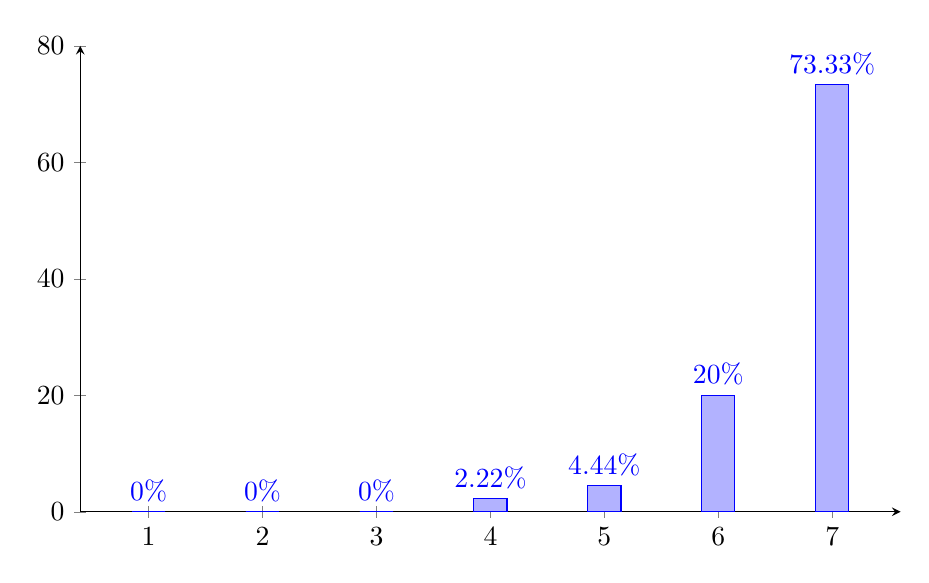
\begin{tikzpicture}
            \begin{axis}[
                height=7.5cm,
                width=12cm,
                ybar,
                bar width=12pt,
                ymin=0,
                ymax=80,
                xtick=data,
                axis x line=bottom,
                axis y line=left,
                enlarge x limits=0.1,
                nodes near coords={\pgfmathprintnumber\pgfplotspointmeta\%},
                legend style={at={(0.5,-0.1)},anchor=north}
            ]
                \addplot coordinates {(1,0) (2,0) (3,0) (4,2.22) (5,4.44) (6,20) (7,73.33)};
            \end{axis}
        \end{tikzpicture}
        \caption*{Responses to the question: ```Privacy is important to me'. Do you agree with this statement?''.}
        \label{fig:survey_s1_q1}
    \end{center}
\end{figure}

\vspace{1cm}

2. ``I know techniques to guarantee privacy and the protection of my data when I use the Internet''. Do you agree with this statement?

\begin{figure}[H]
    \begin{center}
        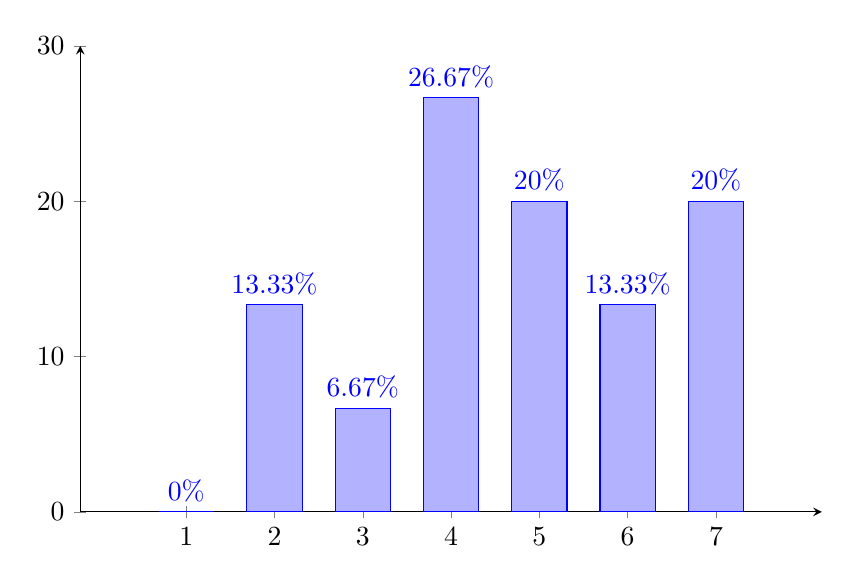
\begin{tikzpicture}
            \begin{axis}[
                height=7.5cm,
                width=11cm,
                ybar,
                bar width=20pt,
                ymin=0,
                ymax=30,
                xtick=data,
                axis x line=bottom,
                axis y line=left,
                enlarge x limits=0.2,
                nodes near coords={\pgfmathprintnumber\pgfplotspointmeta\%}
            ]
                \addplot coordinates {(1,0) (2,13.33) (3,6.67) (4,26.67) (5,20) (6,13.33) (7,20)};
            \end{axis}
        \end{tikzpicture}
        \caption*{Responses to the question: ```I know techniques to guarantee privacy and the protection of my data when I use the Internet'. Do you agree with this statement?''.}
        \label{fig:survey_s1_q2}
    \end{center}
\end{figure}

\clearpage

3. Could you give examples of techniques or strategies you use to guarantee the privacy and protection of your data?

\begin{longtable}{p{3cm} p{13cm}}
    \hline
    \textbf{Participant} & \textbf{Answer} \\
    \hline
    P1 & ``Adblock'' \\
    \hline
    P2 & ``Modo anônimo...'' \\
    \hline
    P3 & ``Ler muito bem as informações ... Peço ajuda a quem percebe muito bem'' \\
    \hline
    P4 & ``Usar palavras passes fortes, não clicar em links, não fornecer dados pessoais, navegar anonimamente'' \\
    \hline
    P5 & ``incognito browser'' \\
    \hline
    P6 & ``Firewall, Virusware, Internet shield, IP anonymous'' \\
    \hline
    P7 & ``Nao inserir dados pessoais em sites que nao sao seguros, verificar sempre protocolos seguranca dos mesmos. Ter copias de seguranca offline de documentos importantes. E nao publucar dados pessoais nas redes sociais.'' \\
    \hline
    P8 & ``perfil privado, anti-vírus, entre outros'' \\
    \hline
    P9 & ``Não fornecer informações pessoais quando não é necessário e optar por produtos de empresas com alguma reputação.'' \\
    \hline
    P10 & ``VPN, modo anónimo do browser, não aceitar cookies'' \\
    \hline
    P11 & ``VPN e Adblock'' \\
    \hline
    P12 & ``antivírus e vpn'' \\
    \hline
    P13 & ``Ter cuidado com inserção de dados pessoais em forms inseguros; Não adicionar convites de estranhos; Ter cuidado com a partilha de informações que possam ser fraudulentas/fake news; Ter muito cuidado nas redes sociais, não se mostrando fotografias ou dados que possam indicar a minha vida privada.'' \\
    \hline
    P14 & ``Utilizar uma VPN'' \\
    \hline
    P15 & ``VPN, firewall, ter diferentes password e que estas sejam longas e complexas'' \\
    \hline
    P16 & ``Palavras-passe; autenticação de dois fatores; antivírus;'' \\
    \hline
    P17 & ``2FA'' \\
    \hline
    P18 & ``modo incognito; não partilhar demasiadas informações quando não é necessário'' \\
    \hline
    P19 & ``Diferentes passwords de acesso'' \\
    \hline
    P20 & ``Não utilizar a 100\% dados reais'' \\
    \hline
    P21 & ``Evitar fazer logins em redes públicas, navegar em modo anónimo e utilizar VPN.'' \\
    \hline
    P22 & ``a minha estrategia e nao dar meus codigos a pessoas estranhas'' \\
    \hline
    P23 & ``Não guardo senhas'' \\
    \hline
    P24 & ``Sempre que são pedidos dados que identifiquem ou que sejam sensíveis opto por interromper a tarefa'' \\
    \hline
    P25 & ``Quando surge a questão se concordo ou não, que sejam utilizados para os diversos fins, concordo ou discordo'' \\
    \hline
    P26 & ``Guardar dados sensíveis em discos externos, uso de antivirus,...'' \\
    \hline
    P27 & ``Trabalhar of line'' \\
    \hline
    P28 & ``VPNs, use `do not track' options whenever possible, and delete your history/cookies'' \\
    \hline
    P29 & ``VPN, virtual machine, sandboxes for specific apps and websites'' \\
    \hline
    P30 & ``adblock, I think I still have some of the worst offenders like doubleclick and facebook routed to 127.0.0.1 in hosts, refuse cookies, used to have js disabled by default too but the web is pretty much unusable now with that setting, because web developers don't know how to do their jobs properly (I'm a web developer).  tbh these are all kind of pointless and certainly do not `guarantee' anything, like just because you click no on the cookie banner, they might still set cookies regardless.  or if they dont use cookies they can use fingerprinting etc etc.  only way to guarantee data protection is not to put it online in the first place.  as search I generally refuse to install random apps (e.g. since covid there is a fad for every bar/restaurant demanding you install their app just to order food/drink, FUCK THAT).  but even then, the game is totally lost already tbh, I'm just pissing in the wind.  google knows everywhere I've been and everything I've searched etc for the last 20 years'' \\
    \hline
    P31 & ``1. I use an alias rather than birth name. 2. I use a service that periodically checks and deletes my data from the top 10 people search sites. 3. I don't perform important functions on mobile devices. 4. Can't read what I've written so I hope this is 4. I don't use any social media that provides real information. 5. I fake all birthdates or important dates. 6. I routinely monitor my credit report. 7. I don't post identifiable information online. 8. I research all online businesses before providing them information.'' \\
    \hline
    P32 & ``Use a VPN. Don't use certain sites and apps. Give fake email addresses and info.'' \\
    \hline
    P33 & ``No account in social media. Rejekt all cookies. No action with real name. No data in the cloud. No picture of me in the net.'' \\
    \hline
    P34 & ``decline on sharing data option for personalized ads, sometimes. i don't usually read the agreement before clicking `i agree to the terms of this agreement''' \\
    \hline
    P35 & ``declining data sharing'' \\
    \hline
    P36 & ``Difficult passwords, anonymity online, antivirus programs'' \\
    \hline
    P37 & ``2 step verification '' \\
    \hline
    P38 & ``security blockers'' \\
    \hline
    P39 & ``think carefully at what info to insert'' \\
    \hline
    P40 & ``VPN, tracker blockers'' \\
    \hline
    P41 & ``VPN, Not signing in with email'' \\
    \hline
    P42-45 & Do not know \\
    \hline
    \caption*{Responses to the question: ``Could you give examples of techniques or strategies you use to guarantee the privacy and protection of your data?''.}
    \label{table:survey_s1_q3}
\end{longtable}

\clearpage

4. Do you think your data privacy is important?

\begin{figure}[H]
    \begin{center}
        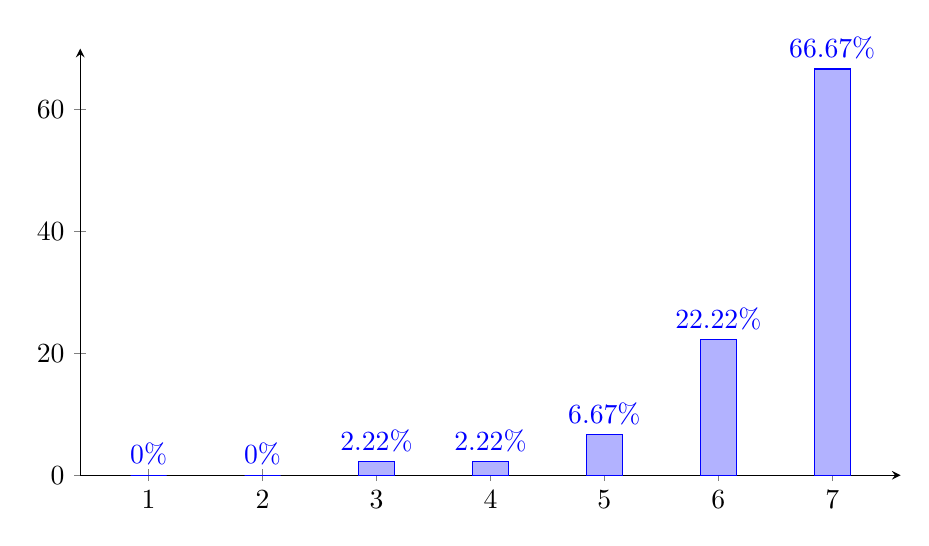
\begin{tikzpicture}
            \begin{axis}[
                height=7cm,
                width=12cm,
                ybar,
                bar width=13pt,
                ymin=0,
                ymax=70,
                xtick=data,
                axis x line=bottom,
                axis y line=left,
                enlarge x limits=0.1,
                nodes near coords={\pgfmathprintnumber\pgfplotspointmeta\%},
                legend style={at={(0.5,-0.1)},anchor=north}
            ]
                \addplot coordinates {(1,0) (2,0) (3,2.22) (4,2.22) (5,6.67) (6,22.22) (7,66.67)};
            \end{axis}
        \end{tikzpicture}
        \caption*{Responses to the question: ``Do you think your data privacy is important?''.}
        \label{fig:survey_s1_q4}
    \end{center}
\end{figure}

5. How do you define data (or digital) privacy?

\begin{longtable}{p{3cm} p{13cm}}
    \hline
    \textbf{Participant} & \textbf{Answer} \\
    \hline
    P1 & ``Tudo o que impede que a minha informação esteja disponível'' \\
    \hline
    P2 & ``Guardar os nossos dados só para nós'' \\
    \hline
    P3 & ``A capacidade que um indivíduo tem de controlar a exposição das suas informações na internet.'' \\
    \hline
    P4 & ``Forma de garantir que a identidade seja adulterada'' \\
    \hline
    P5 & ``Confidencialidade '' \\
    \hline
    P6 & ``Nao divulgação a terceiros de tudo aquilo que seja considerado pessoal'' \\
    \hline
    P7 & ``Capacidade de escolher que dados de um sistema podem ser compartilhados com terceiros.'' \\
    \hline
    P8 & ``Que os meus dados pessoais não são partilhados com ninguém'' \\
    \hline
    P9 & ``A partilha de dados sensíveis com pessoal autorizado'' \\
    \hline
    P10 & ``os dados de um utilizador devem estar apenas ao alcance do mesmo'' \\
    \hline
    P11 & ``Informações e valores onde não são dadas ao público nem partilhados por pessoas e utilizadores que não deviam ter acesso.'' \\
    \hline
    P12 & ``Segurança e anonimato.'' \\
    \hline
    P13 & ``Incapacidade de alguém alheio aceder aos meus dados'' \\
    \hline
    P14 & ``não partilha de dados para fins além dos descritos e com outras entidades'' \\
    \hline
    P15 & ``É uma das coisas mais importantes.'' \\
    \hline
    P16 & ``eu defino  como  uma maneira da pessoa se proteger dos borloes'' \\
    \hline
    P17 & ``Apenas tem acesso a informação privada as pessoas ou entidades que eu voluntariamente e conscientemente autorizo'' \\
    \hline
    P18 & ``O não uso de dados pessoais'' \\
    \hline
    P19 & ``A não divulgação para outros fins, que os permitidos'' \\
    \hline
    P20 & ``Os dados devem estar encriptados por chaves públicas e privadas.'' \\
    \hline
    P21 & ``Ninguém ter acesso aos meus `trabalhos' no momento de produção'' \\
    \hline
    P22 & ``basically anything that can identify you and impact your life off of the computer'' \\
    \hline
    P23 & ``Ensuring data privacy is minimizing the amount and scope of data that can be collected by any party from you, your devices, or anything you use or do on your devices'' \\
    \hline
    P24 & ``that my data is not bought/sold/mined etc without consent'' \\
    \hline
    P25 & ``This is a difficult question as so much has changed within my lifetime. Before the internet, you could find out information on a person just by going to a court house but needed specific information to do so. Then we also had the phonebooks delivered that gave you an actual address and person's name. To me, this definition would be, you are entitled to privacy unless you post the information online - then all bets are off - you post it, you've infringed on your own privacy.'' \\
    \hline
    P26 & ``The right not to have your data disclosed, accessed, or shared.'' \\
    \hline
    P27 & ``hacker prevention i suppose. true digital privacy doesn't exist for me, because big companies like facebook data mine, which i can't do nothing about if i want to still use the platform.'' \\
    \hline
    P28 & ``personal data not being shared'' \\
    \hline
    P29 & ``My data is my own and not accessible to others without my consent'' \\
    \hline
    P30 & ``no personal info gets shared to a third party without your consent'' \\
    \hline
    P31 & ``how many ppl see ur data'' \\
    \hline
    P32 & ``That I have control over how my personal data are being used and processed'' \\
    \hline
    P33 & ``Companies not using my info for other purposes'' \\
    \hline
    P34 & ``data remaining private and confidential to the data-owner'' \\
    \hline
    P35 & ``dData privacy is how much ownership I have of my own data, and knowing who collects it and for what purpose. '' \\
    \hline
    P36 & ``Anonimato'' \\
    \hline
    P37-45 & Do not know \\
    \hline
    \caption*{Responses to the question: ``How do you define data (or digital) privacy?''.}
    \label{table:survey_s1_q5}
\end{longtable}

\clearpage

6. Do you think your data privacy is relevant nowadays?

\begin{figure}[H]
    \begin{center}
        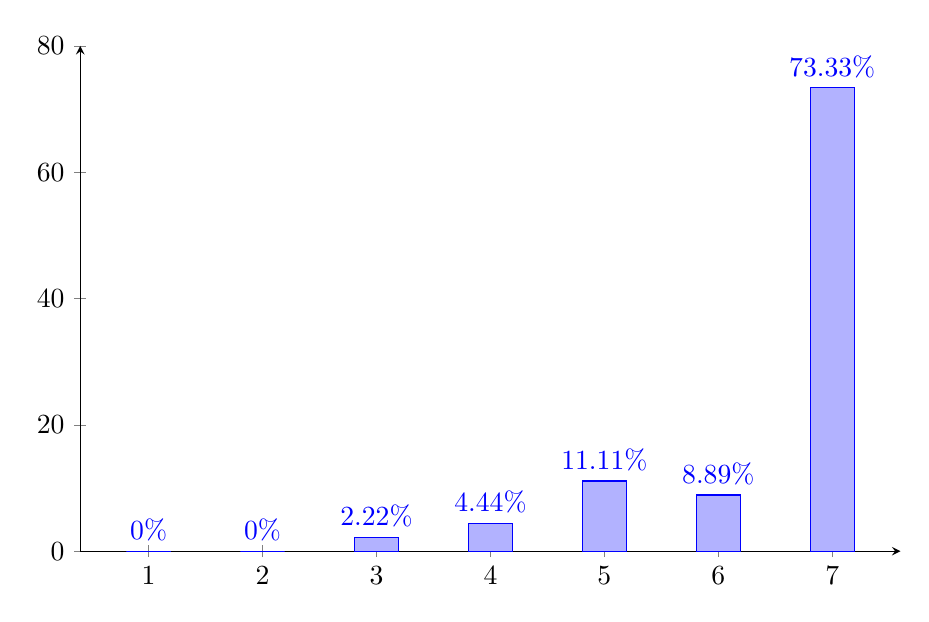
\begin{tikzpicture}
            \begin{axis}[
                height=8cm,
                width=12cm,
                ybar,
                bar width=16pt,
                ymin=0,
                ymax=80,
                xtick=data,
                axis x line=bottom,
                axis y line=left,
                enlarge x limits=0.1,
                nodes near coords={\pgfmathprintnumber\pgfplotspointmeta\%},
                legend style={at={(0.5,-0.1)},anchor=north}
            ]
                \addplot coordinates {(1,0) (2,0) (3,2.22) (4,4.44) (5,11.11) (6,8.89) (7,73.33)};
            \end{axis}
        \end{tikzpicture}
        \caption*{Responses to the question: ``Do you think your data privacy is relevant nowadays?''.}
        \label{fig:survey_s1_q6}
    \end{center}
\end{figure}

\vspace{2cm}

7. ``Data privacy is a human right''. Do you agree with this statement?

\begin{figure}[H]
    \begin{center}
        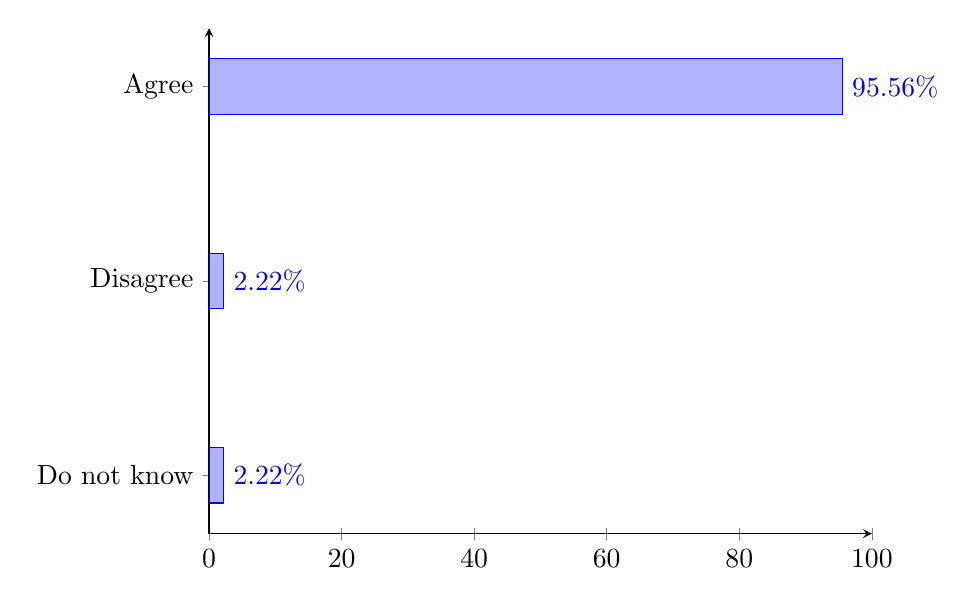
\begin{tikzpicture}
            \begin{axis}[
                height=8cm,
                width=10cm,
                xbar,
                symbolic y coords={Do not know,Disagree,Agree},
                bar width=20pt,
                ytick=data,
                axis x line=bottom,
                axis y line=left,
                xmin=0,
                xmax=100,
                enlarge y limits=0.15,
                nodes near coords={\pgfmathprintnumber\pgfplotspointmeta\%},
                legend style={at={(0.5,-0.1)},anchor=north}
            ]
                \addplot coordinates {(2.22,Do not know) (2.22,Disagree) (95.56,Agree)};
            \end{axis}
        \end{tikzpicture}
        \caption*{Responses to the question: ```Data privacy is a human right'. Do you agree with this statement?''.}
        \label{fig:survey_s1_q7}
    \end{center}
\end{figure}

\clearpage

8. ``Data privacy is a consumer right''. Do you agree with this statement?

\begin{figure}[H]
    \begin{center}
        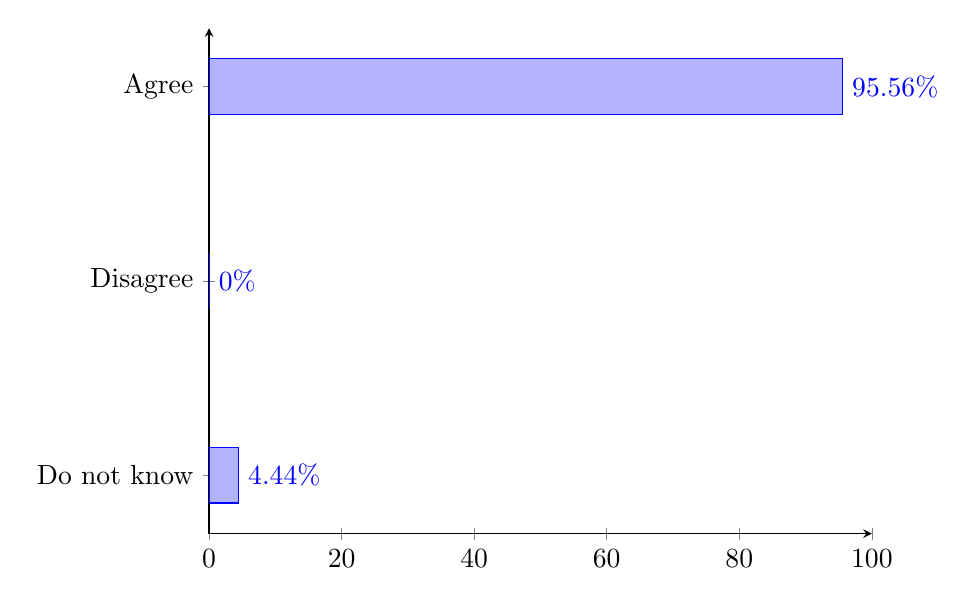
\begin{tikzpicture}
            \begin{axis}[
                height=8cm,
                width=10cm,
                xbar,
                symbolic y coords={Do not know,Disagree,Agree},
                bar width=20pt,
                ytick=data,
                axis x line=bottom,
                axis y line=left,
                xmin=0,
                xmax=100,
                enlarge y limits=0.15,
                nodes near coords={\pgfmathprintnumber\pgfplotspointmeta\%},
                legend style={at={(0.5,-0.1)},anchor=north}
            ]
                \addplot coordinates {(4.44,Do not know) (0,Disagree) (95.56,Agree)};
            \end{axis}
        \end{tikzpicture}
        \caption*{Responses to the question: ```Data privacy is a consumer right'. Do you agree with this statement?''.}
        \label{fig:survey_s1_q8}
    \end{center}
\end{figure}

\vspace{2cm}

9. In your opinion, are security and privacy synonymous?

\begin{figure}[H]
    \centering
    \begin{tikzpicture}
        \pie[explode = 0.1]{46.67/No,
            53.33/Yes}
    \end{tikzpicture}
    \caption*{Responses to the question: ``In your opinion, are security and privacy synonymous?''.}
    \label{fig:survey_s1_q9}
\end{figure}

\clearpage

10. How familiar are you with the following terms?

\begin{figure}[H]
    \begin{center}
        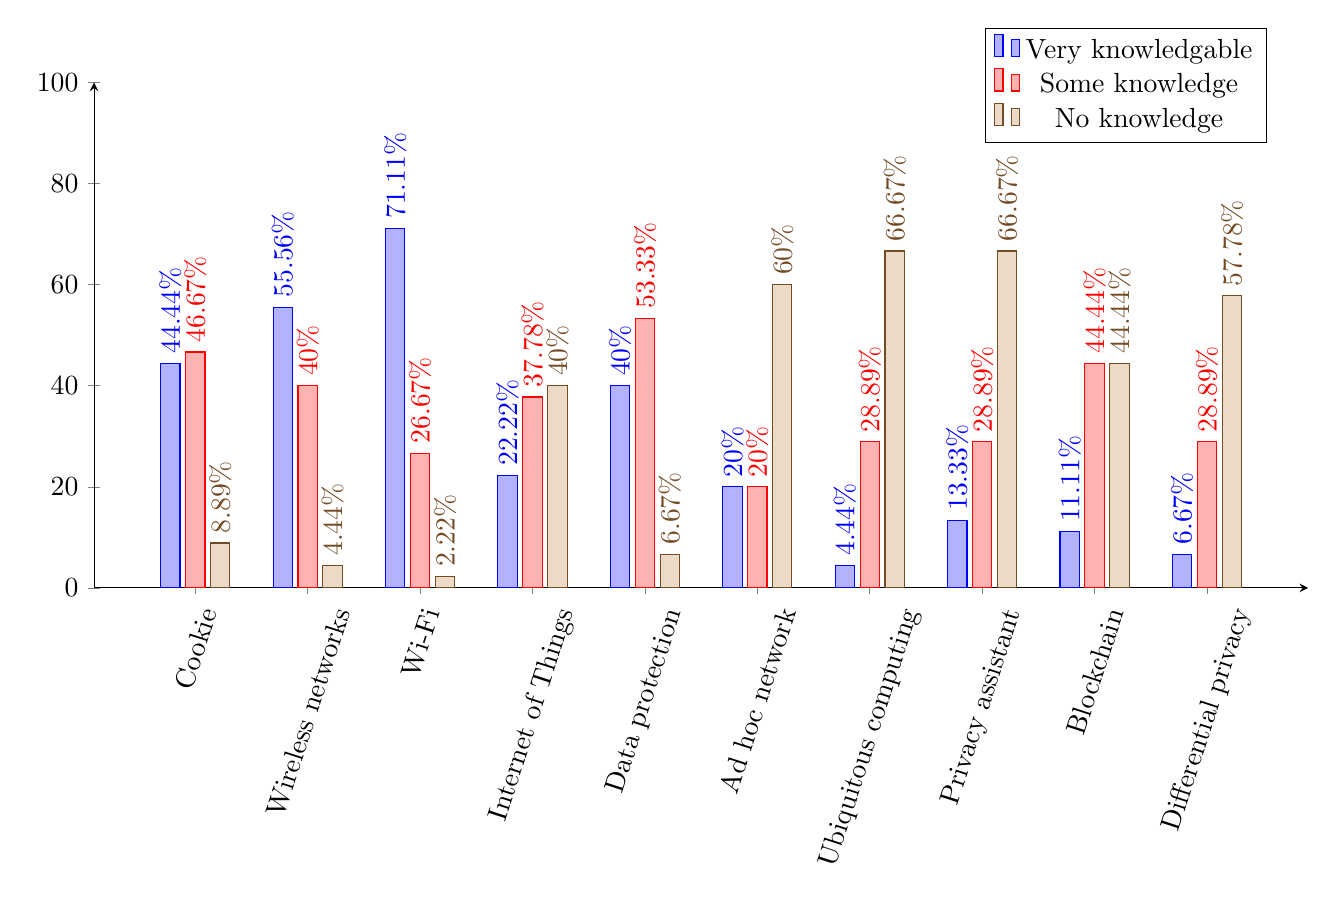
\begin{tikzpicture}
            \begin{axis}[
                height=8cm,
                width=17cm,
                symbolic x coords={Cookie, Wireless networks,Wi-Fi,Internet of Things,Data protection,Ad hoc network,Ubiquitous computing,Privacy assistant,Blockchain,Differential privacy},
                ybar,
                bar width=7pt,
                ymin=0,
                ymax=100,
                xticklabel style={rotate=72},
                axis x line=bottom,
                axis y line=left,
                enlarge x limits=0.1,
                nodes near coords={\pgfmathprintnumber\pgfplotspointmeta\%},
                every node near coord/.append style={rotate=90, anchor=west},
                legend style={at={(0.85,0.88)},anchor=south}
            ]
                \addplot coordinates {(Cookie,44.44) (Wireless networks,55.56) (Wi-Fi,71.11) (Internet of Things,22.22) (Data protection,40) (Ad hoc network,20) (Ubiquitous computing,4.44) (Privacy assistant,13.33) (Blockchain,11.11) (Differential privacy,6.67)};
                \addlegendentry{Very knowledgable}
                \addplot coordinates {(Cookie,46.67) (Wireless networks,40) (Wi-Fi,26.67) (Internet of Things,37.78) (Data protection,53.33) (Ad hoc network,20) (Ubiquitous computing,28.89) (Privacy assistant,28.89) (Blockchain,44.44) (Differential privacy,28.89)};
                \addlegendentry{Some knowledge}
                \addplot coordinates {(Cookie,8.89) (Wireless networks,4.44) (Wi-Fi,2.22) (Internet of Things,40) (Data protection,6.67) (Ad hoc network,60) (Ubiquitous computing,66.67) (Privacy assistant,66.67) (Blockchain,44.44) (Differential privacy,57.78)};
                \addlegendentry{No knowledge}
            \end{axis}
        \end{tikzpicture}
        \caption*{Responses to the question: ``How familiar are you with the following [IT] terms?''.}
        \label{fig:survey_s1_q10}
    \end{center}
\end{figure}

11. Do you think your data is stored/collected when you use the internet?

\begin{figure}[H]
    \centering
    \begin{tikzpicture}
        \pie[explode = 0.1]{4.44/I do not know,
            8.89/No,
            86.67/Yes}
    \end{tikzpicture}
    \caption*{Responses to the question: ``Do you think your data is stored/collected when you use the internet?''.}
    \label{fig:survey_s1_q11}
\end{figure}

12. What means do you think are used to collect your data?

\begin{figure}[H]
    \begin{center}
        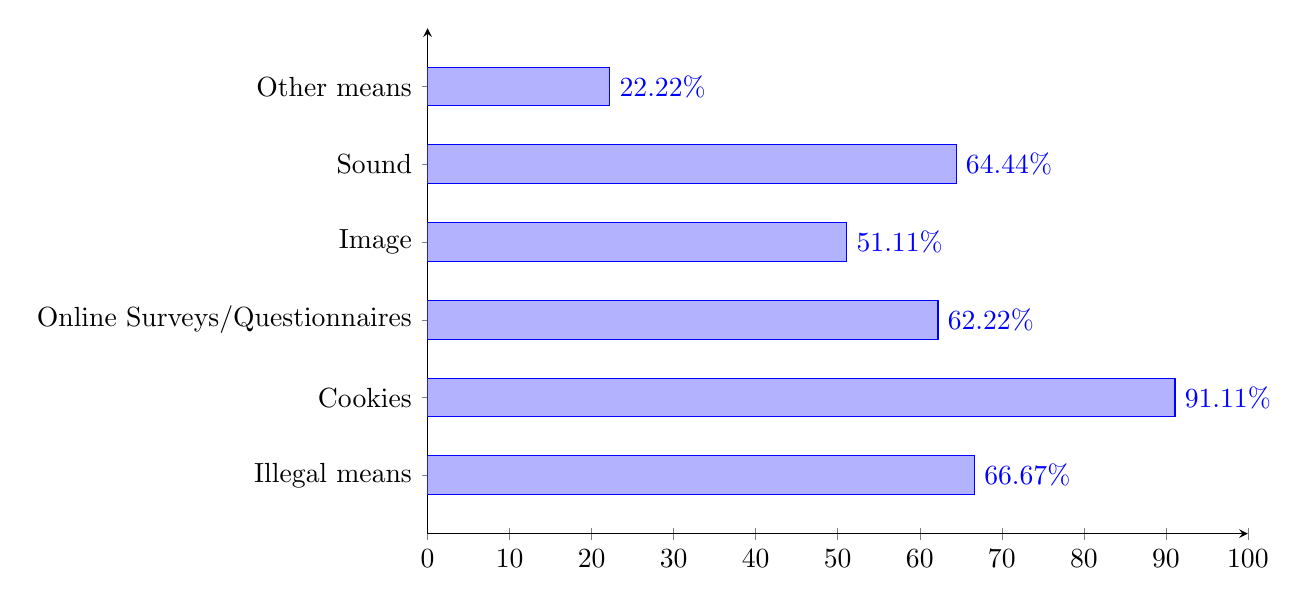
\begin{tikzpicture}
            \begin{axis}[
                height=8cm,
                width=12cm,
                xbar,
                symbolic y coords={Illegal means,Cookies,Online Surveys/Questionnaires,Image,Sound,Other means},
                bar width=14pt,
                ytick=data,
                axis x line=bottom,
                axis y line=left,
                xmin=0,
                xmax=100,
                enlarge y limits=0.15,
                nodes near coords={\pgfmathprintnumber\pgfplotspointmeta\%},
            ]
                \addplot coordinates {(66.67,Illegal means) (91.11,Cookies) (62.22,Online Surveys/Questionnaires) (51.11,Image) (64.44,Sound) (22.22,Other means)};
            \end{axis}
        \end{tikzpicture}
        \caption*{Responses to the question: ``What means do you think are used to collect your data?''.}
        \label{fig:survey_s1_q12}
    \end{center}
\end{figure}

\vspace{2cm}

13. What kind of information can be extracted using the collected data?

\begin{figure}[H]
    \begin{center}
        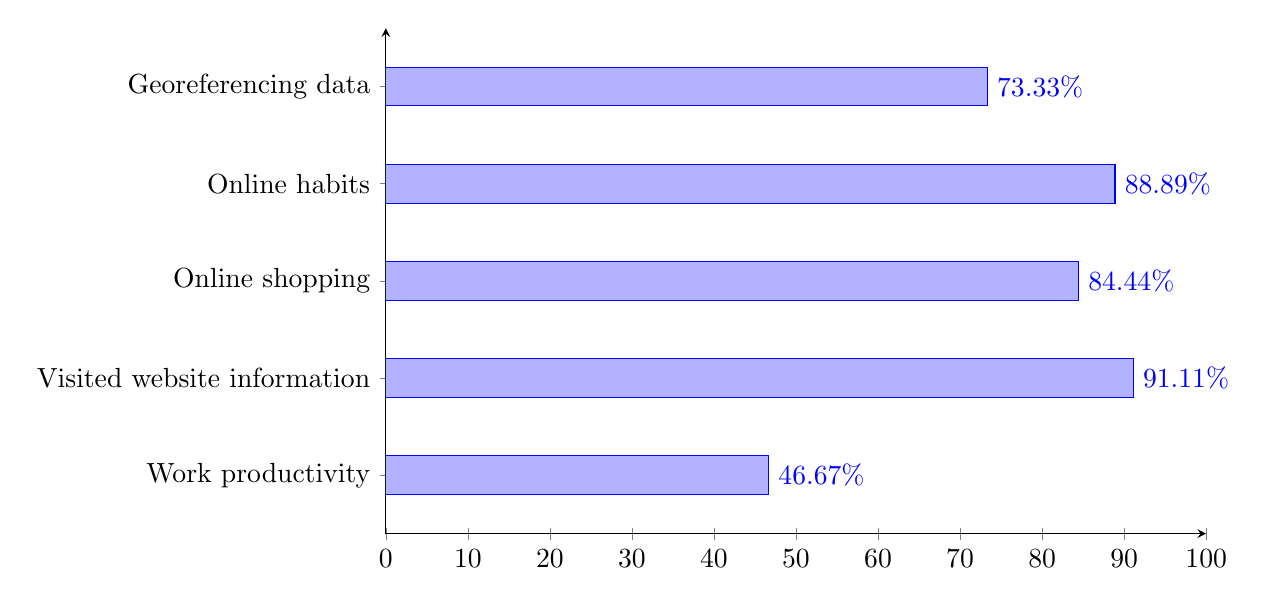
\begin{tikzpicture}
            \begin{axis}[
                height=8cm,
                width=12cm,
                xbar,
                symbolic y coords={Work productivity,Visited website information,Online shopping,Online habits,Georeferencing data},
                bar width=14pt,
                ytick=data,
                axis x line=bottom,
                axis y line=left,
                xmin=0,
                xmax=100,
                enlarge y limits=0.15,
                nodes near coords={\pgfmathprintnumber\pgfplotspointmeta\%},
            ]
                \addplot coordinates {(46.67,Work productivity) (91.11,Visited website information) (84.44,Online shopping) (88.89,Online habits) (73.33,Georeferencing data)};
            \end{axis}
        \end{tikzpicture}
        \caption*{Responses to the question: ``What kind of information can be extracted using the collected data?''.}
        \label{fig:survey_s1_q13}
    \end{center}
\end{figure}

\clearpage

14. For what purposes can organizations use your data?

\begin{figure}[H]
    \begin{center}
        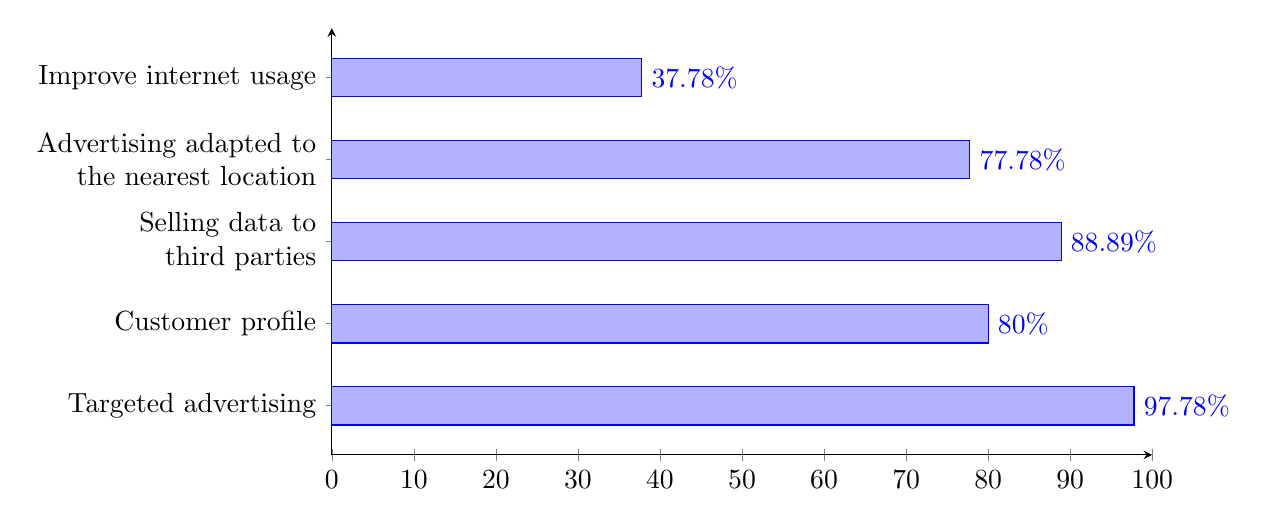
\begin{tikzpicture}
            \begin{axis}[
                height=7cm,
                width=12cm,
                xbar,
                symbolic y coords={Targeted advertising,Customer profile,Selling data to third parties,Advertising adapted to the nearest location,Improve internet usage},
                yticklabels={
                    Targeted advertising,
                    Customer profile,
                    Selling data to\\third parties,
                    Advertising adapted to\\the nearest location,
                    Improve internet usage,
                },
                yticklabel style={align=right},
                bar width=14pt,
                ytick=data,
                axis x line=bottom,
                axis y line=left,
                xmin=0,
                xmax=100,
                enlarge y limits=0.15,
                nodes near coords={\pgfmathprintnumber\pgfplotspointmeta\%},
            ]
                \addplot coordinates {(97.78,Targeted advertising) (80,Customer profile) (88.89,Selling data to third parties) (77.78,Advertising adapted to the nearest location) (37.78,Improve internet usage)};
            \end{axis}
        \end{tikzpicture}
        \caption*{Responses to the question: ``For what purposes can organizations use your data?''.}
        \label{fig:survey_s1_q14}
    \end{center}
\end{figure}

15. Which organizations do you consider to have the best privacy behaviour?

\begin{figure}[H]
    \begin{center}
        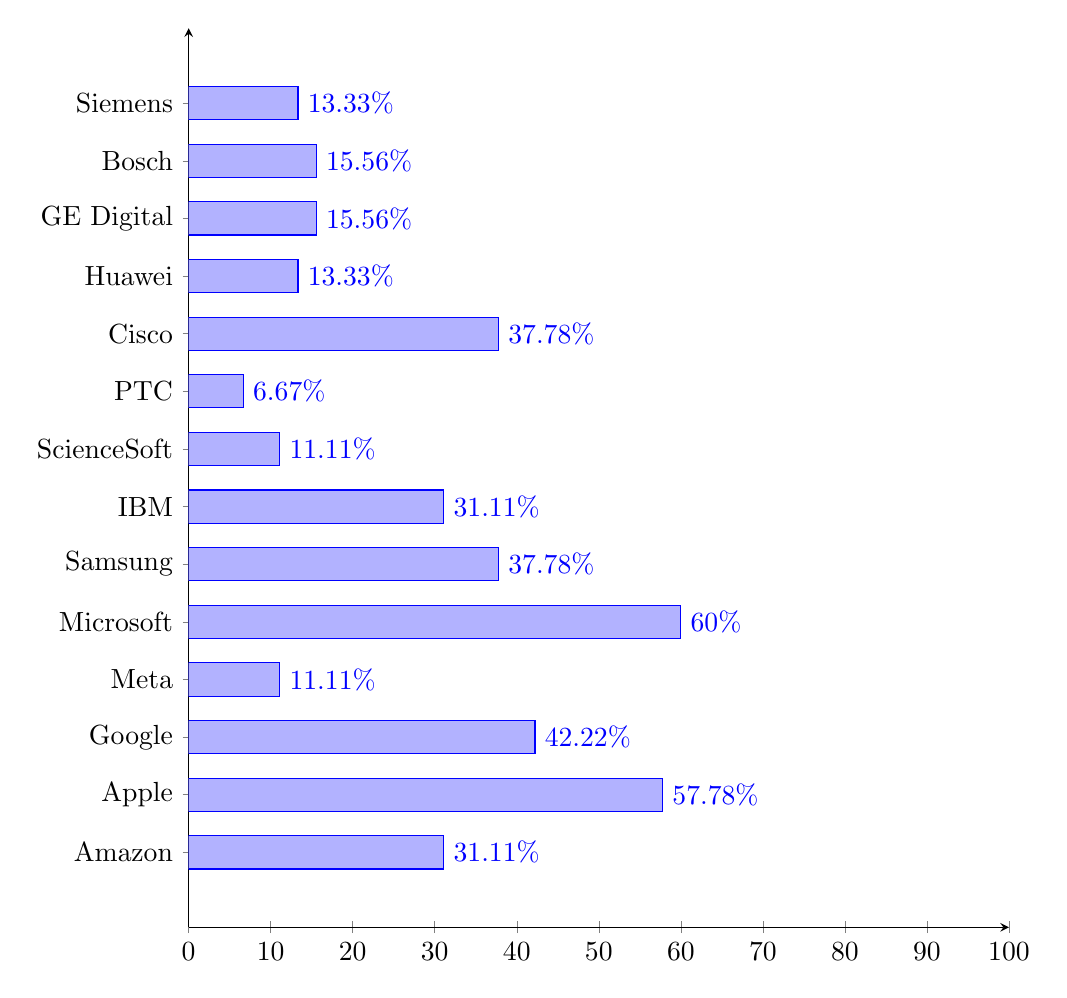
\begin{tikzpicture}
            \begin{axis}[
                height=13cm,
                width=12cm,
                xbar,
                symbolic y coords={Amazon,Apple,Google,Meta,Microsoft,Samsung,IBM,ScienceSoft,PTC,Cisco,Huawei,GE Digital,Bosch,Siemens},
                bar width=12pt,
                ytick=data,
                axis x line=bottom,
                axis y line=left,
                xmin=0,
                xmax=100,
                enlarge y limits=0.1,
                nodes near coords={\pgfmathprintnumber\pgfplotspointmeta\%},
            ]
                \addplot coordinates {(31.11,Amazon) (57.78,Apple) (42.22,Google) (11.11,Meta) (60,Microsoft) (37.78,Samsung) (31.11,IBM) (11.11,ScienceSoft) (6.67,PTC) (37.78,Cisco) (13.33,Huawei) (15.56,GE Digital) (15.56,Bosch) (13.33,Siemens)};
            \end{axis}
        \end{tikzpicture}
        \caption*{Responses to the question: ``Which organizations do you consider to have the best privacy behaviour?''.}
        \label{fig:survey_s1_q15}
    \end{center}
\end{figure}

16. Which organizations do you consider to have the worst privacy behaviour?

\begin{figure}[H]
    \begin{center}
        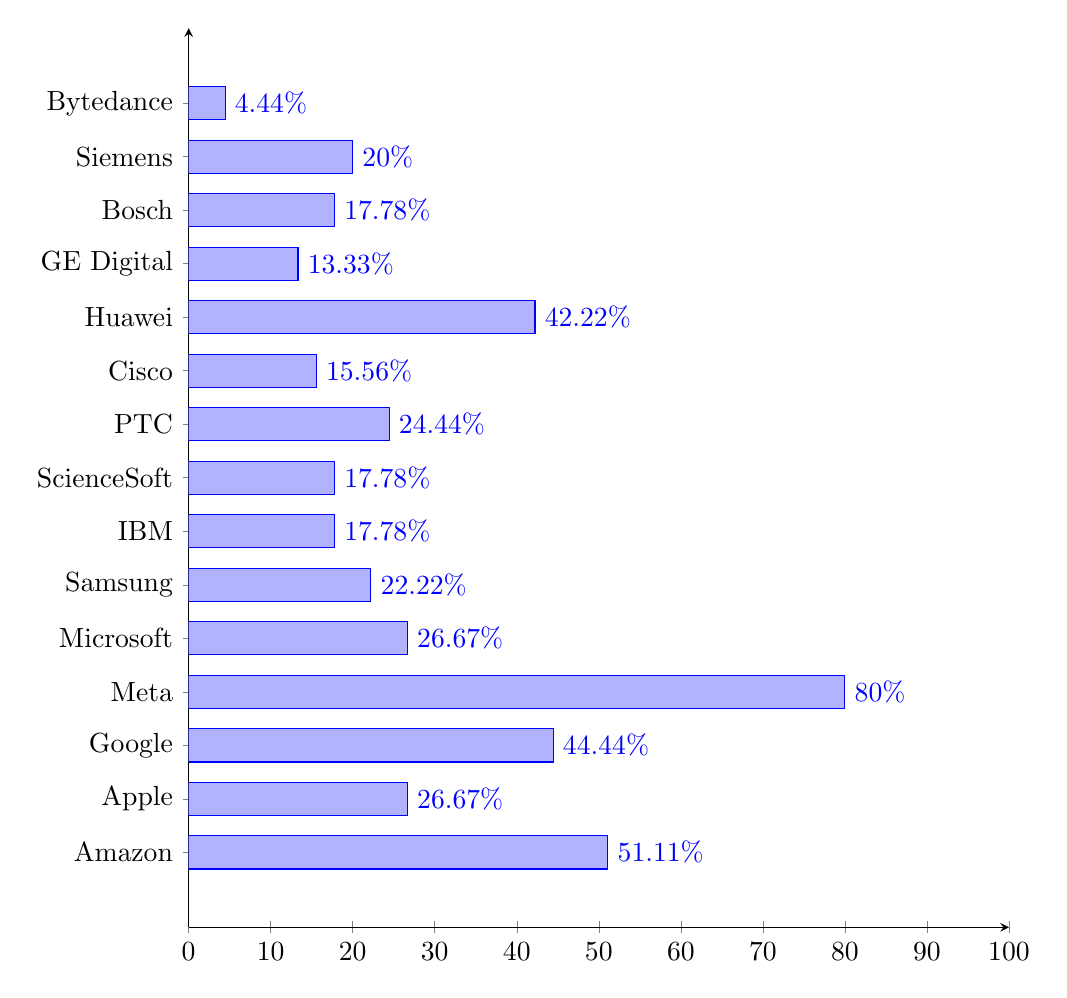
\begin{tikzpicture}
            \begin{axis}[
                height=13cm,
                width=12cm,
                xbar,
                symbolic y coords={Amazon,Apple,Google,Meta,Microsoft,Samsung,IBM,ScienceSoft,PTC,Cisco,Huawei,GE Digital,Bosch,Siemens,Bytedance},
                bar width=12pt,
                ytick=data,
                axis x line=bottom,
                axis y line=left,
                xmin=0,
                xmax=100,
                enlarge y limits=0.1,
                nodes near coords={\pgfmathprintnumber\pgfplotspointmeta\%},
            ]
                \addplot coordinates {(51.11,Amazon) (26.67,Apple) (44.44,Google) (80,Meta) (26.67,Microsoft) (22.22,Samsung) (17.78,IBM) (17.78,ScienceSoft) (24.44,PTC) (15.56,Cisco) (42.22,Huawei) (13.33,GE Digital) (17.78,Bosch) (20,Siemens) (4.44,Bytedance)};
            \end{axis}
        \end{tikzpicture}
        \caption*{Responses to the question: ``Which organizations do you consider to have the worst privacy behaviour?''.}
        \label{fig:survey_s1_q16}
    \end{center}
\end{figure}

17. During your day-to-day life, how often do you use your phone to access the internet?

\begin{figure}[H]
    \begin{center}
        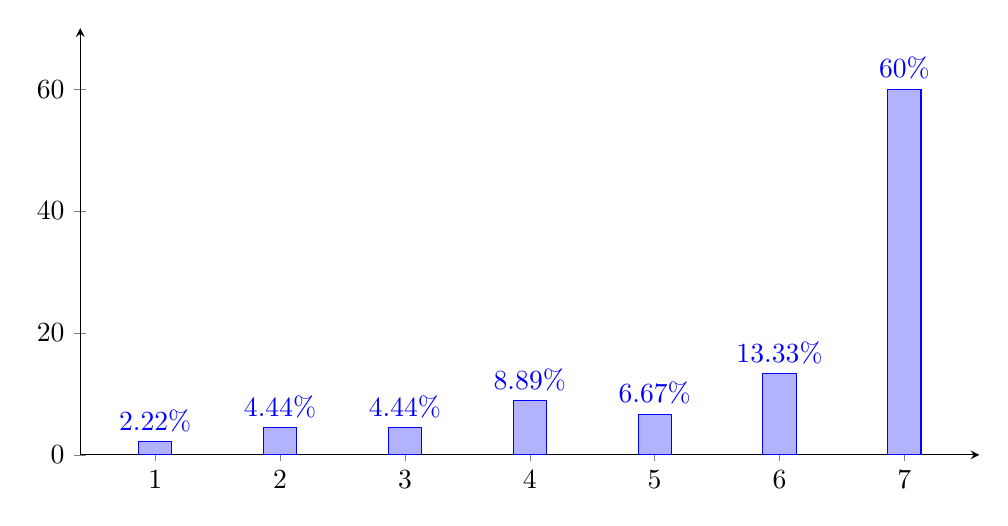
\begin{tikzpicture}
            \begin{axis}[
                height=7cm,
                width=13cm,
                ybar,
                bar width=12pt,
                ymin=0,
                ymax=70,
                % ytick=data,
                xtick=data,
                axis x line=bottom,
                axis y line=left,
                enlarge x limits=0.1,
                nodes near coords={\pgfmathprintnumber\pgfplotspointmeta\%},
            ]
                \addplot coordinates {(1,2.22) (2,4.44) (3,4.44) (4,8.89) (5,6.67) (6,13.33) (7,60)};
            \end{axis}
        \end{tikzpicture}
        \caption*{Responses to the question: ``During your day-to-day life, how often do you use your phone to access the internet?''.}
        \label{fig:survey_s1_q17}
    \end{center}
\end{figure}

18. ``I am concerned about my privacy when using my mobile phone when accessing the internet''. Do you agree with this statement?

\begin{figure}[H]
    \begin{center}
        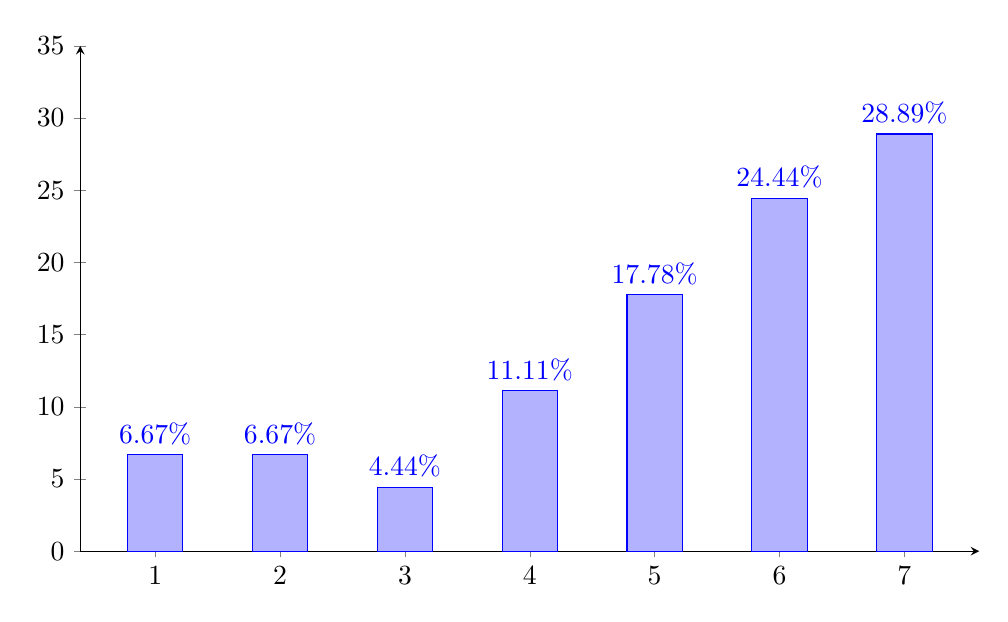
\begin{tikzpicture}
            \begin{axis}[
                height=8cm,
                width=13cm,
                ybar,
                bar width=20pt,
                ymin=0,
                ymax=35,
                % ytick=data,
                xtick=data,
                axis x line=bottom,
                axis y line=left,
                enlarge x limits=0.1,
                nodes near coords={\pgfmathprintnumber\pgfplotspointmeta\%},
            ]
                \addplot coordinates {(1,6.67) (2,6.67) (3,4.44) (4,11.11) (5,17.78) (6,24.44) (7,28.89)};
            \end{axis}
        \end{tikzpicture}
        \caption*{Responses to the question: ```I am concerned about my privacy when using my mobile phone when accessing the internet'. Do you agree with this statement?''.}
        \label{fig:survey_s1_q18}
    \end{center}
\end{figure}

\vspace{2cm}

19. ``I consider that accessing the internet through my phone is safer than through a computer''. Do you agree with this statement?

\begin{figure}[H]
    \begin{center}
        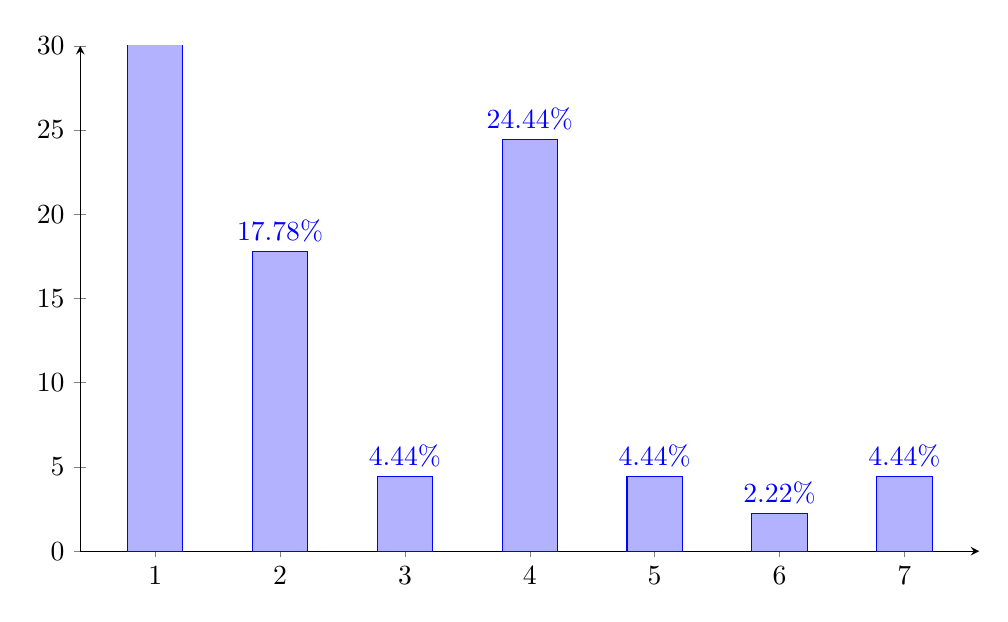
\begin{tikzpicture}
            \begin{axis}[
                height=8cm,
                width=13cm,
                ybar,
                bar width=20pt,
                ymin=0,
                ymax=30,
                % ytick=data,
                xtick=data,
                axis x line=bottom,
                axis y line=left,
                enlarge x limits=0.1,
                nodes near coords={\pgfmathprintnumber\pgfplotspointmeta\%},
            ]
                \addplot coordinates {(1,42.22) (2,17.78) (3,4.44) (4,24.44) (5,4.44) (6,2.22) (7,4.44)};
            \end{axis}
        \end{tikzpicture}
        \caption*{Responses to the question: ```I consider that accessing the internet through my phone is safer than through a computer'. Do you agree with this statement?''.}
        \label{fig:survey_s1_q19}
    \end{center}
\end{figure}

\clearpage

20. ``I try to block the collection of data from applications installed on my phone''. Do you agree with this statement?

\begin{figure}[H]
    \begin{center}
        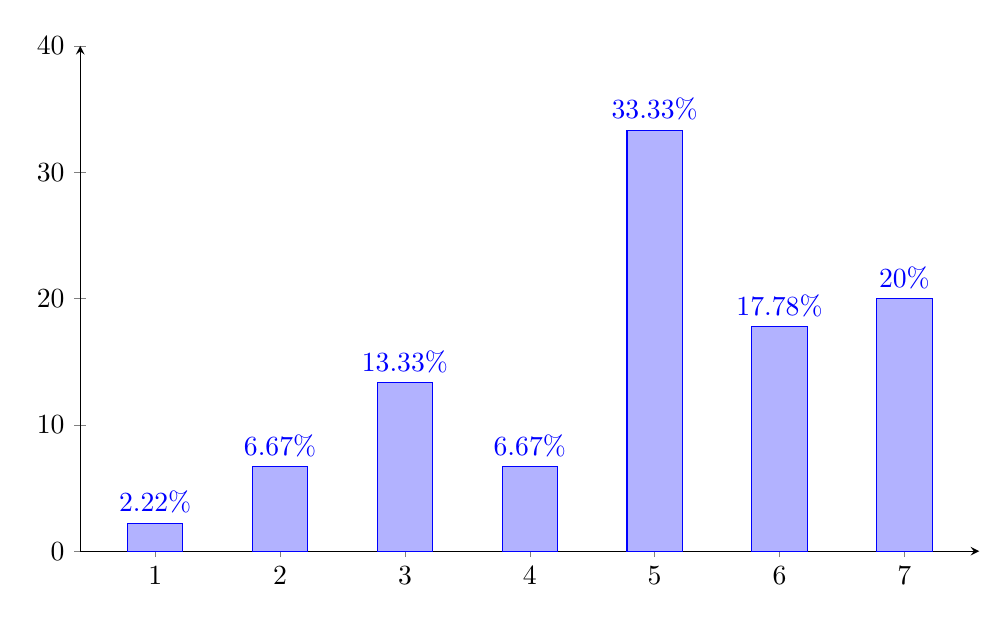
\begin{tikzpicture}
            \begin{axis}[
                height=8cm,
                width=13cm,
                ybar,
                bar width=20pt,
                ymin=0,
                ymax=40,
                % ytick=data,
                xtick=data,
                axis x line=bottom,
                axis y line=left,
                enlarge x limits=0.1,
                nodes near coords={\pgfmathprintnumber\pgfplotspointmeta\%},
            ]
                \addplot coordinates {(1,2.22) (2,6.67) (3,13.33) (4,6.67) (5,33.33) (6,17.78) (7,20)};
            \end{axis}
        \end{tikzpicture}
        \caption*{Responses to the question: ```I try to block the collection of data from applications installed on my phone'. Do you agree with this statement?''.}
        \label{fig:survey_s1_q20}
    \end{center}
\end{figure}

\vspace{2cm}

21. When using a website, do you usually read the privacy policy?

\begin{figure}[H]
    \begin{center}
        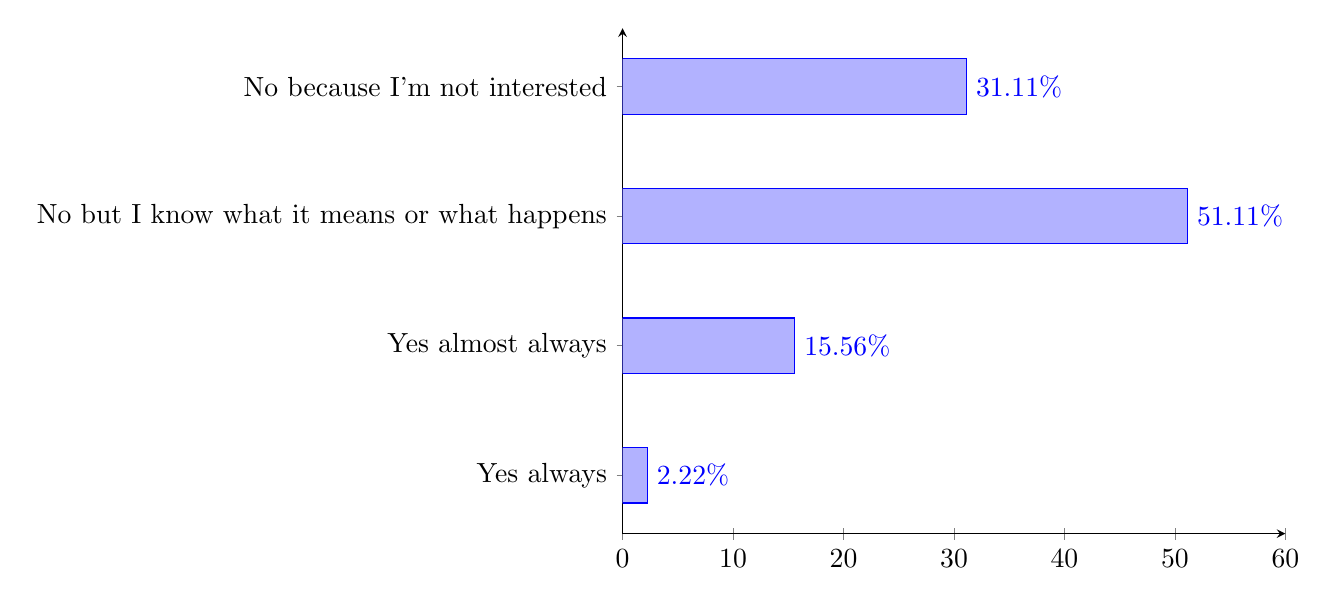
\begin{tikzpicture}
            \begin{axis}[
                height=8cm,
                width=10cm,
                xbar,
                symbolic y coords={Yes always,Yes almost always,No but I know what it means or what happens,No because I'm not interested},
                bar width=20pt,
                ytick=data,
                axis x line=bottom,
                axis y line=left,
                xmin=0,
                xmax=60,
                enlarge y limits=0.15,
                nodes near coords={\pgfmathprintnumber\pgfplotspointmeta\%},
            ]
                \addplot coordinates {(2.22,Yes always) (15.56,Yes almost always) (51.11,No but I know what it means or what happens) (31.11,No because I'm not interested)};
            \end{axis}
        \end{tikzpicture}
        \caption*{Responses to the question: ``When using a website, do you usually read the privacy policy?''.}
        \label{fig:survey_s1_q21}
    \end{center}
\end{figure}

\clearpage

22. How often do you allow the use of cookies?

\begin{figure}[H]
    \begin{center}
        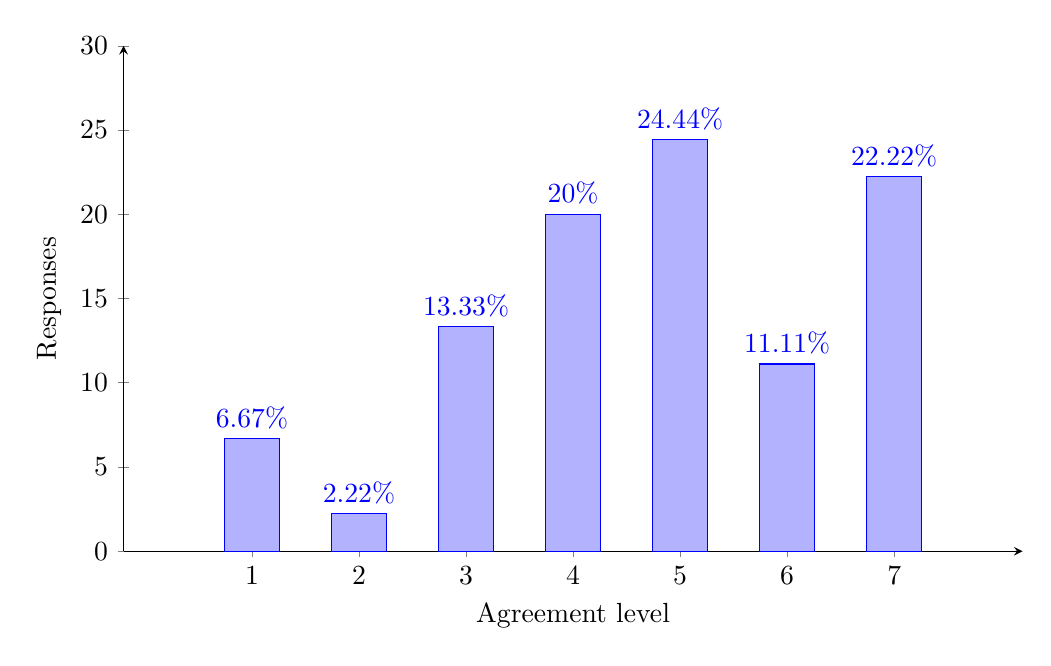
\begin{tikzpicture}
            \begin{axis}[
                height=8cm,
                width=13cm,
                ybar,
                xlabel={Agreement level},
                ylabel={Responses},
                % ytick=\empty,
                xtick=data,
                ymin=0,
                ymax=30,
                axis x line=bottom,
                axis y line=left,
                enlarge x limits=0.2,
                bar width=20pt,
                nodes near coords={\pgfmathprintnumber\pgfplotspointmeta\%}
            ]
                \addplot coordinates {(1,6.67) (2,2.22) (3,13.33) (4,20) (5,24.44) (6,11.11) (7,22.22)};
            \end{axis}
        \end{tikzpicture}
        \caption*{Responses to the question: ``How often do you allow the use of cookies?''.}
        \label{fig:survey_s1_q22}
    \end{center}
\end{figure}

\vspace{2cm}

23. When you accept / become aware of the cookies policy, why do you take this decision?

\begin{figure}[H]
    \begin{center}
        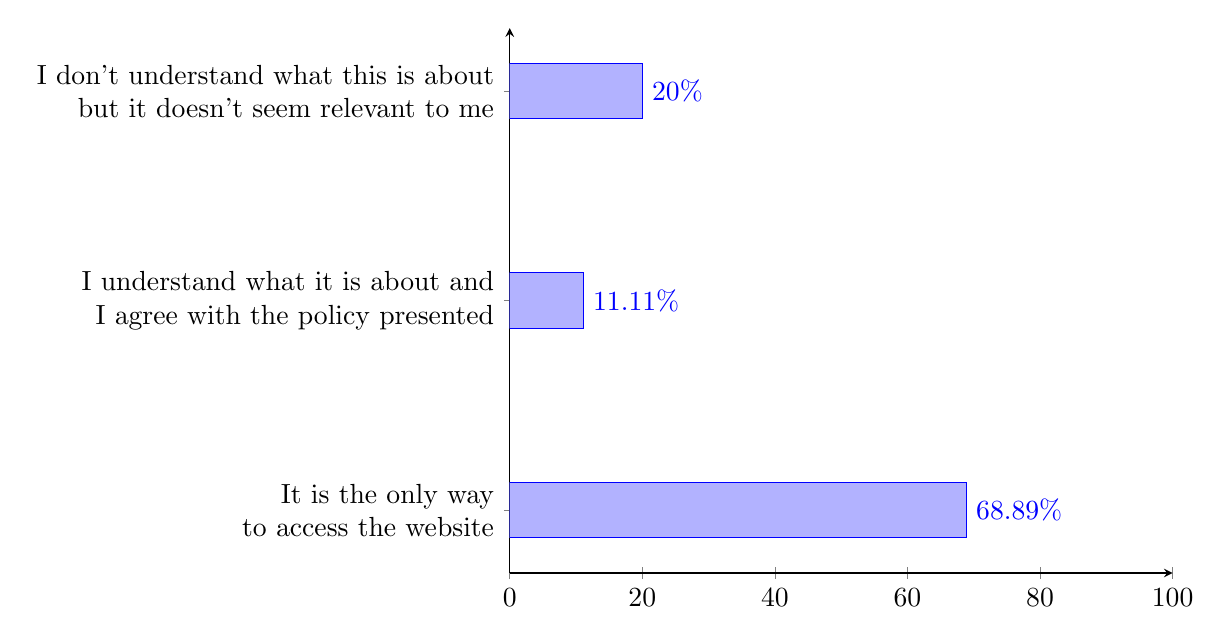
\begin{tikzpicture}
            \begin{axis}[
                height=8.5cm,
                width=10cm,
                xbar,
                xmin=0,
                xmax=100,
                symbolic y coords={It is the only way to access the website,I understand what it is about and I agree with the policy presented,I don't understand what this is about but it doesn't seem relevant to me},
                ytick=data,
                yticklabels={
                    It is the only way\\to access the website,
                    I understand what it is about and\\I agree with the policy presented,
                    I don't understand what this is about\\but it doesn't seem relevant to me,
                },
                yticklabel style={align=right},
                bar width=20pt,
                axis x line=bottom,
                axis y line=left,
                enlarge y limits=0.15,
                nodes near coords={\pgfmathprintnumber\pgfplotspointmeta\%},
                % ticklabel style={font=\tiny},
            ]
            \addplot coordinates {(68.89,It is the only way to access the website) (11.11,I understand what it is about and I agree with the policy presented) (20,I don't understand what this is about but it doesn't seem relevant to me)};
            \end{axis}
        \end{tikzpicture}
        \caption*{Responses to the question: ``When you accept / become aware of the cookies policy, why do you take this decision?''.}
        \label{fig:survey_s1_q23}
    \end{center}
\end{figure}

\clearpage

24. Are you aware of the concept of ``profiling'' or ``automated processing of personal information''?

\begin{figure}[H]
    \centering
    \begin{tikzpicture}
        \pie[explode = 0.1]{51.11/No,
            48.89/Yes}
    \end{tikzpicture}
    \caption*{Responses to the question: ``Are you aware of the concept of `profiling' or `automated processing of personal information'?''.}
    \label{fig:survey_s2_q24}
\end{figure}

\vspace{1cm}

25. Do you consider that your internet activity contributes to the development of profiling?\\

\begin{figure}[H]
    \centering
    \begin{tikzpicture}
        \pie[explode = 0.1]{33.33/Do not know,
            8.89/No,
            57.78/Yes}
    \end{tikzpicture}
    \caption*{Responses to the question: ``Do you consider that your internet activity contributes to the development of profiling?''.}
    \label{fig:survey_s2_q25}
\end{figure}

26. Are you aware of regulations such as the General Data Protection Regulation or the California Consumer Privacy Act?

\begin{figure}[H]
    \begin{center}
        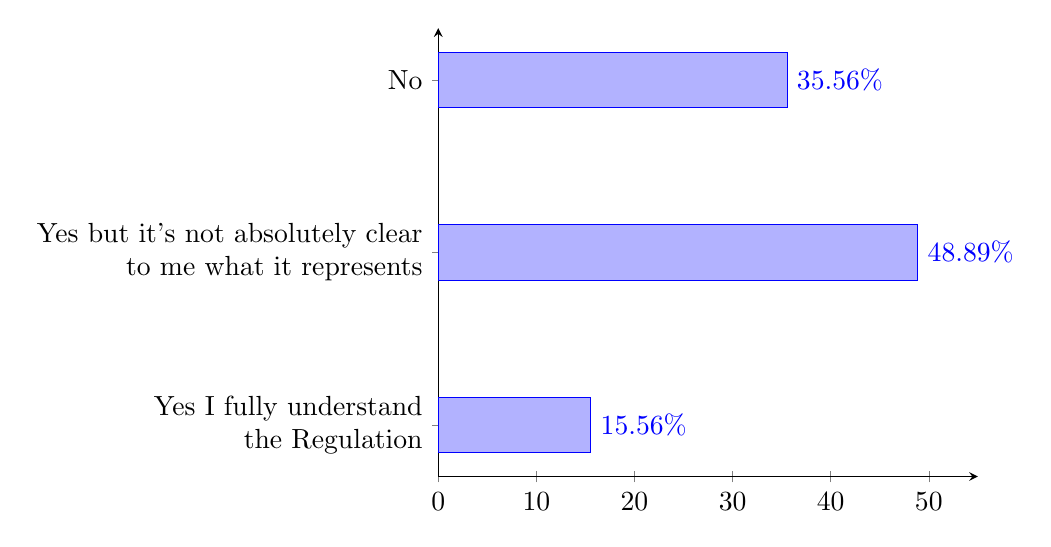
\begin{tikzpicture}
            \begin{axis}[
                xbar,
                symbolic y coords={Yes I fully understand the Regulation,Yes but it's not absolutely clear to me what it represents,No},
                bar width=20pt,
                ytick=data,
                yticklabels={
                    Yes I fully understand\\the Regulation,
                    Yes but it's not absolutely clear\\to me what it represents,
                    No,
                },
                yticklabel style={align=right},
                axis x line=bottom,
                axis y line=left,
                xmin=0,
                xmax=55,
                enlarge y limits=0.15,
                nodes near coords={\pgfmathprintnumber\pgfplotspointmeta\%},
            ]
                \addplot coordinates {(15.56,Yes I fully understand the Regulation) (48.89,Yes but it's not absolutely clear to me what it represents) (35.56,No)};
            \end{axis}
        \end{tikzpicture}
        \caption*{Responses to the question: ``Are you aware of regulations such as the General Data Protection Regulation or the California Consumer Privacy Act?''.}
        \label{fig:survey_s1_q26}
    \end{center}
\end{figure}

27. If you answered yes, how did you learn about the `General Data Protection Regulation' or the `California Consumer Privacy Act'?

\begin{figure}[H]
    \begin{center}
        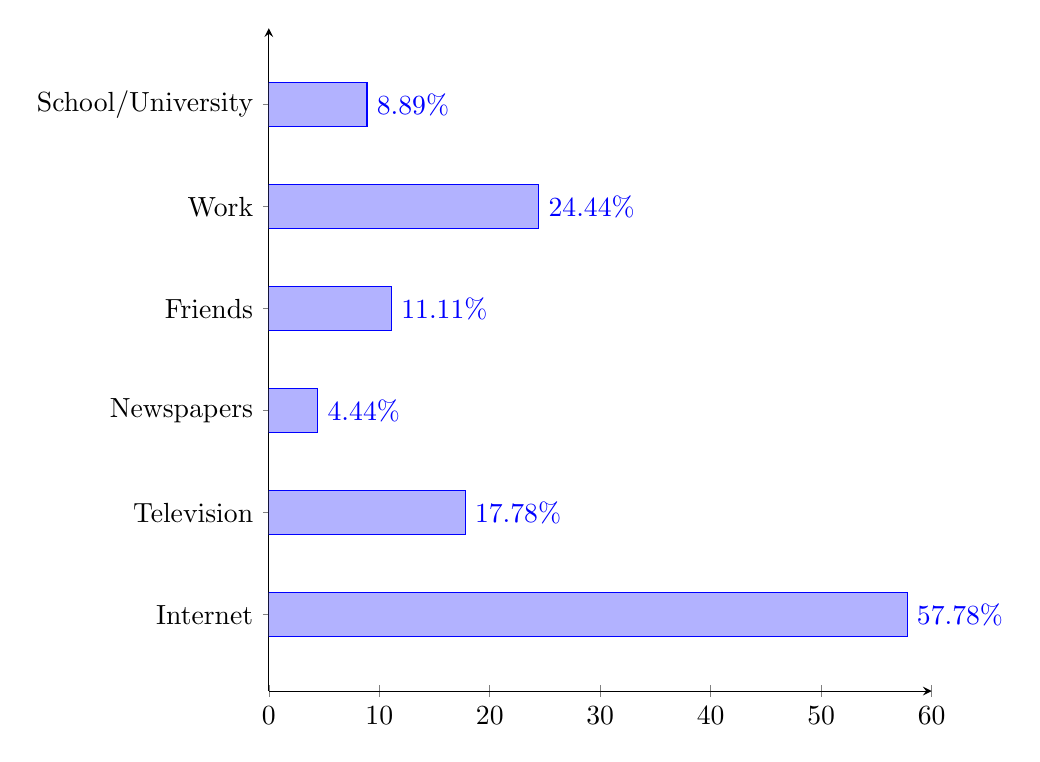
\begin{tikzpicture}
            \begin{axis}[
                height=10cm,
                width=10cm,
                xbar,
                symbolic y coords={Internet,Television,Newspapers,Friends,Work,School/University},
                bar width=16pt,
                ytick=data,
                axis x line=bottom,
                axis y line=left,
                xmin=0,
                xmax=60,
                enlarge y limits=0.15,
                nodes near coords={\pgfmathprintnumber\pgfplotspointmeta\%},
            ]
                \addplot coordinates {(57.78,Internet) (17.78,Television) (4.44,Newspapers) (11.11,Friends) (24.44,Work) (8.89,School/University)};
            \end{axis}
        \end{tikzpicture}
        \caption*{Responses to the question: ``If you answered yes, how did you learn about the `General Data Protection Regulation' or the `California Consumer Privacy Act'?''.}
        \label{fig:survey_s1_q27}
    \end{center}
\end{figure}

28. Are you interested in finding out more about regulations or legislation related to digital privacy?

\begin{figure}[H]
    \begin{center}
        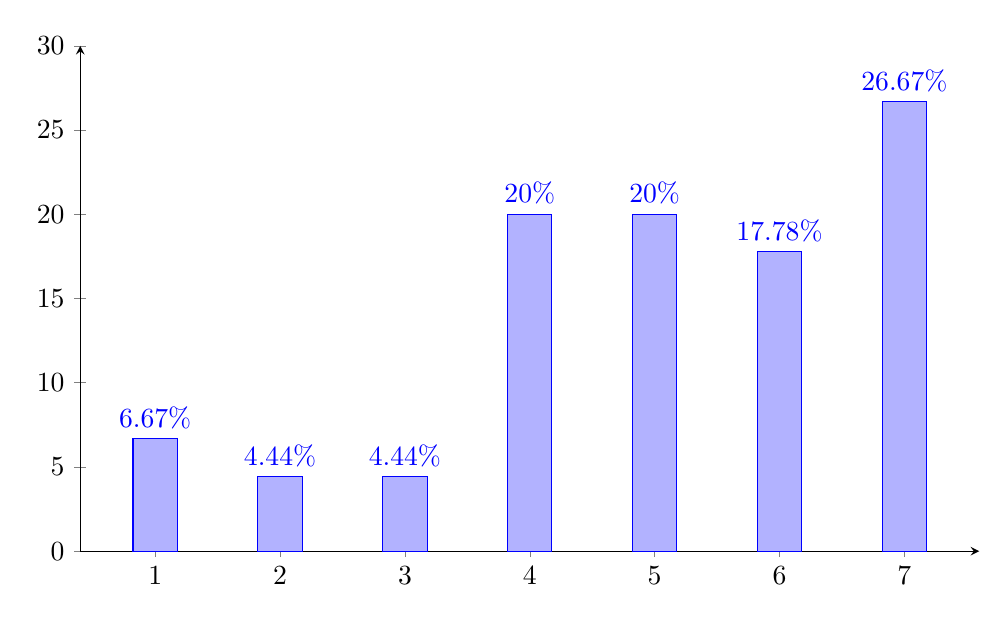
\begin{tikzpicture}
            \begin{axis}[
                height=8cm,
                width=13cm,
                ybar,
                bar width=16pt,
                ymin=0,
                ymax=30,
                % ytick=\empty,
                xtick=data,
                axis x line=bottom,
                axis y line=left,
                enlarge x limits=0.1,
                nodes near coords={\pgfmathprintnumber\pgfplotspointmeta\%},
            ]
                \addplot coordinates {(1,6.67) (2,4.44) (3,4.44) (4,20) (5,20) (6,17.78) (7,26.67)};
            \end{axis}
        \end{tikzpicture}
        \caption*{Responses to the question: ``Are you interested in finding out more about regulations or legislation related to digital privacy?''.}
        \label{fig:survey_s1_q28}
    \end{center}
\end{figure}

29. According to the General Data Protection Regulation, personal data is:

\begin{figure}[H]
    \begin{center}
        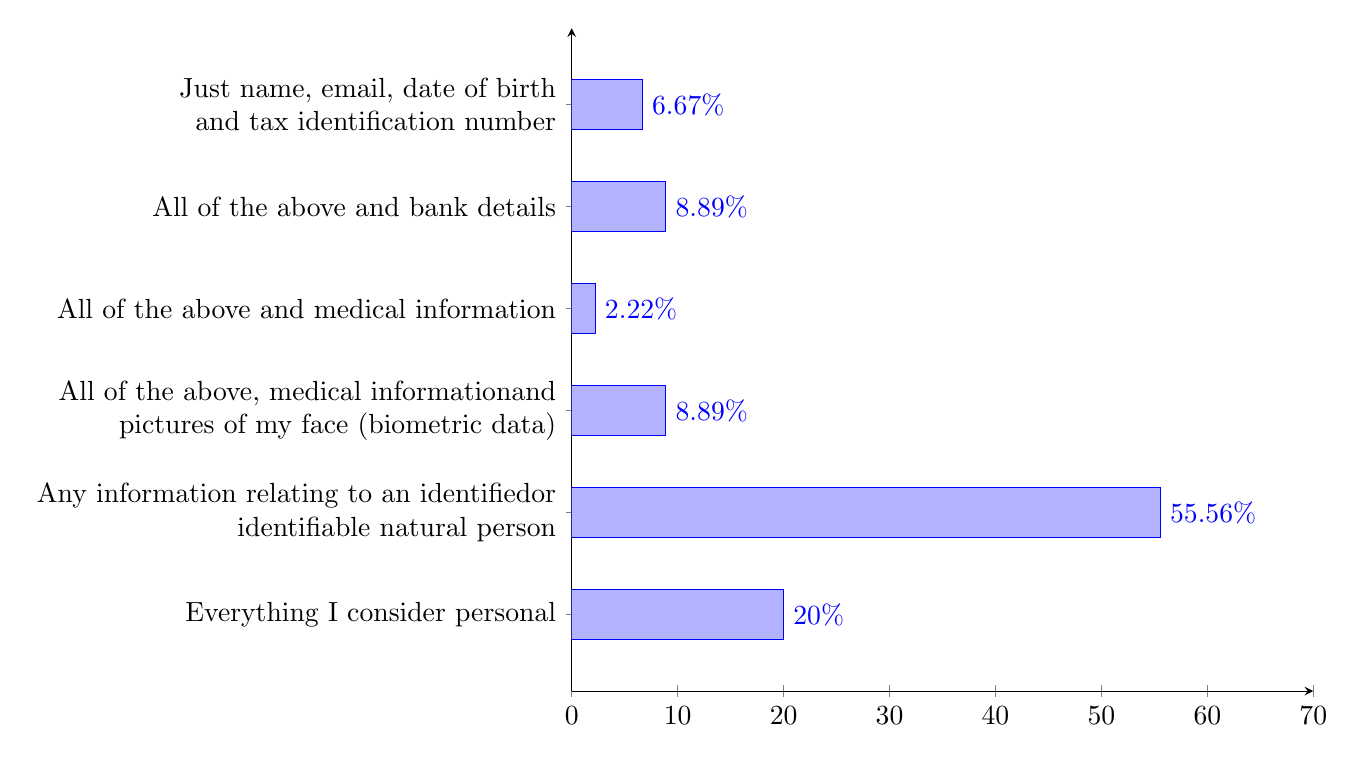
\begin{tikzpicture}
            \begin{axis}[
                height=10cm,
                width=11cm,
                xbar,
                symbolic y coords={Everything I consider personal,Any information relating to an identifiedor identifiable natural person,{All of the above, medical informationand pictures of my face (biometric data)},All of the above and medical information,All of the above and bank details,{Just name, email, date of birth and tax identification number}},
                bar width=18pt,
                ytick=data,
                yticklabels={
                    Everything I consider personal,
                    Any information relating to an identifiedor\\identifiable natural person,
                    {All of the above, medical informationand\\pictures of my face (biometric data)},
                    All of the above and medical information,
                    All of the above and bank details,
                    {Just name, email, date of birth\\and tax identification number},
                },
                yticklabel style={align=right},
                axis x line=bottom,
                axis y line=left,
                xmin=0,
                xmax=70,
                enlarge y limits=0.15,
                nodes near coords={\pgfmathprintnumber\pgfplotspointmeta\%},
            ]
                \addplot coordinates {(20,Everything I consider personal) (55.56,Any information relating to an identifiedor identifiable natural person) (8.89,{All of the above, medical informationand pictures of my face (biometric data)}) (2.22,All of the above and medical information) (8.89,All of the above and bank details) (6.67,{Just name, email, date of birth and tax identification number})};
            \end{axis}
        \end{tikzpicture}
        \caption*{Responses to the question: ``According to the General Data Protection Regulation, personal data is:''.}
        \label{fig:survey_s1_q29}
    \end{center}
\end{figure}

30. ``My data was more protected after the implementation of regulations such as the General Data Protection Regulation''. Do you agree with this statement?

\begin{figure}[H]
    \begin{center}
        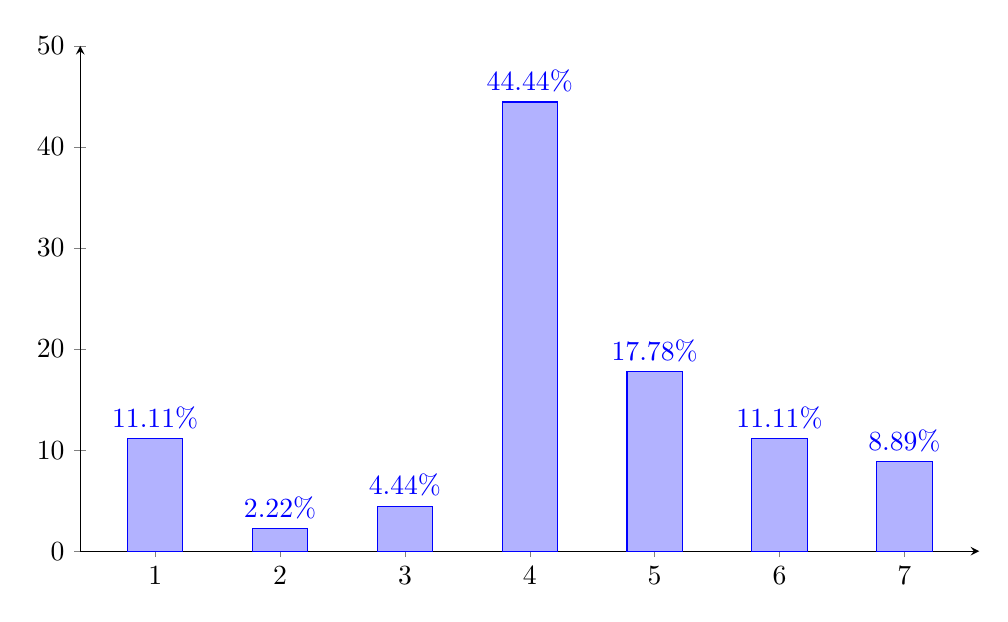
\begin{tikzpicture}
            \begin{axis}[
                height=8cm,
                width=13cm,
                ybar,
                bar width=20pt,
                ymin=0,
                ymax=50,
                % ytick=\empty,
                xtick=data,
                axis x line=bottom,
                axis y line=left,
                enlarge x limits=0.1,
                nodes near coords={\pgfmathprintnumber\pgfplotspointmeta\%},
            ]
                \addplot coordinates {(1,11.11) (2,2.22) (3,4.44) (4,44.44) (5,17.78) (6,11.11) (7,8.89)};
            \end{axis}
        \end{tikzpicture}
        \caption*{Responses to the question: ```My data was more protected after the implementation of regulations such as the General Data Protection Regulation'. Do you agree with this statement?''.}
        \label{fig:survey_s1_q30}
    \end{center}
\end{figure}

\clearpage

\subsection*{Section 2: Disposition for sharing personal information}

1. What kind of personal information are you willing to share at any time?

\begin{figure}[H]
    \begin{center}
        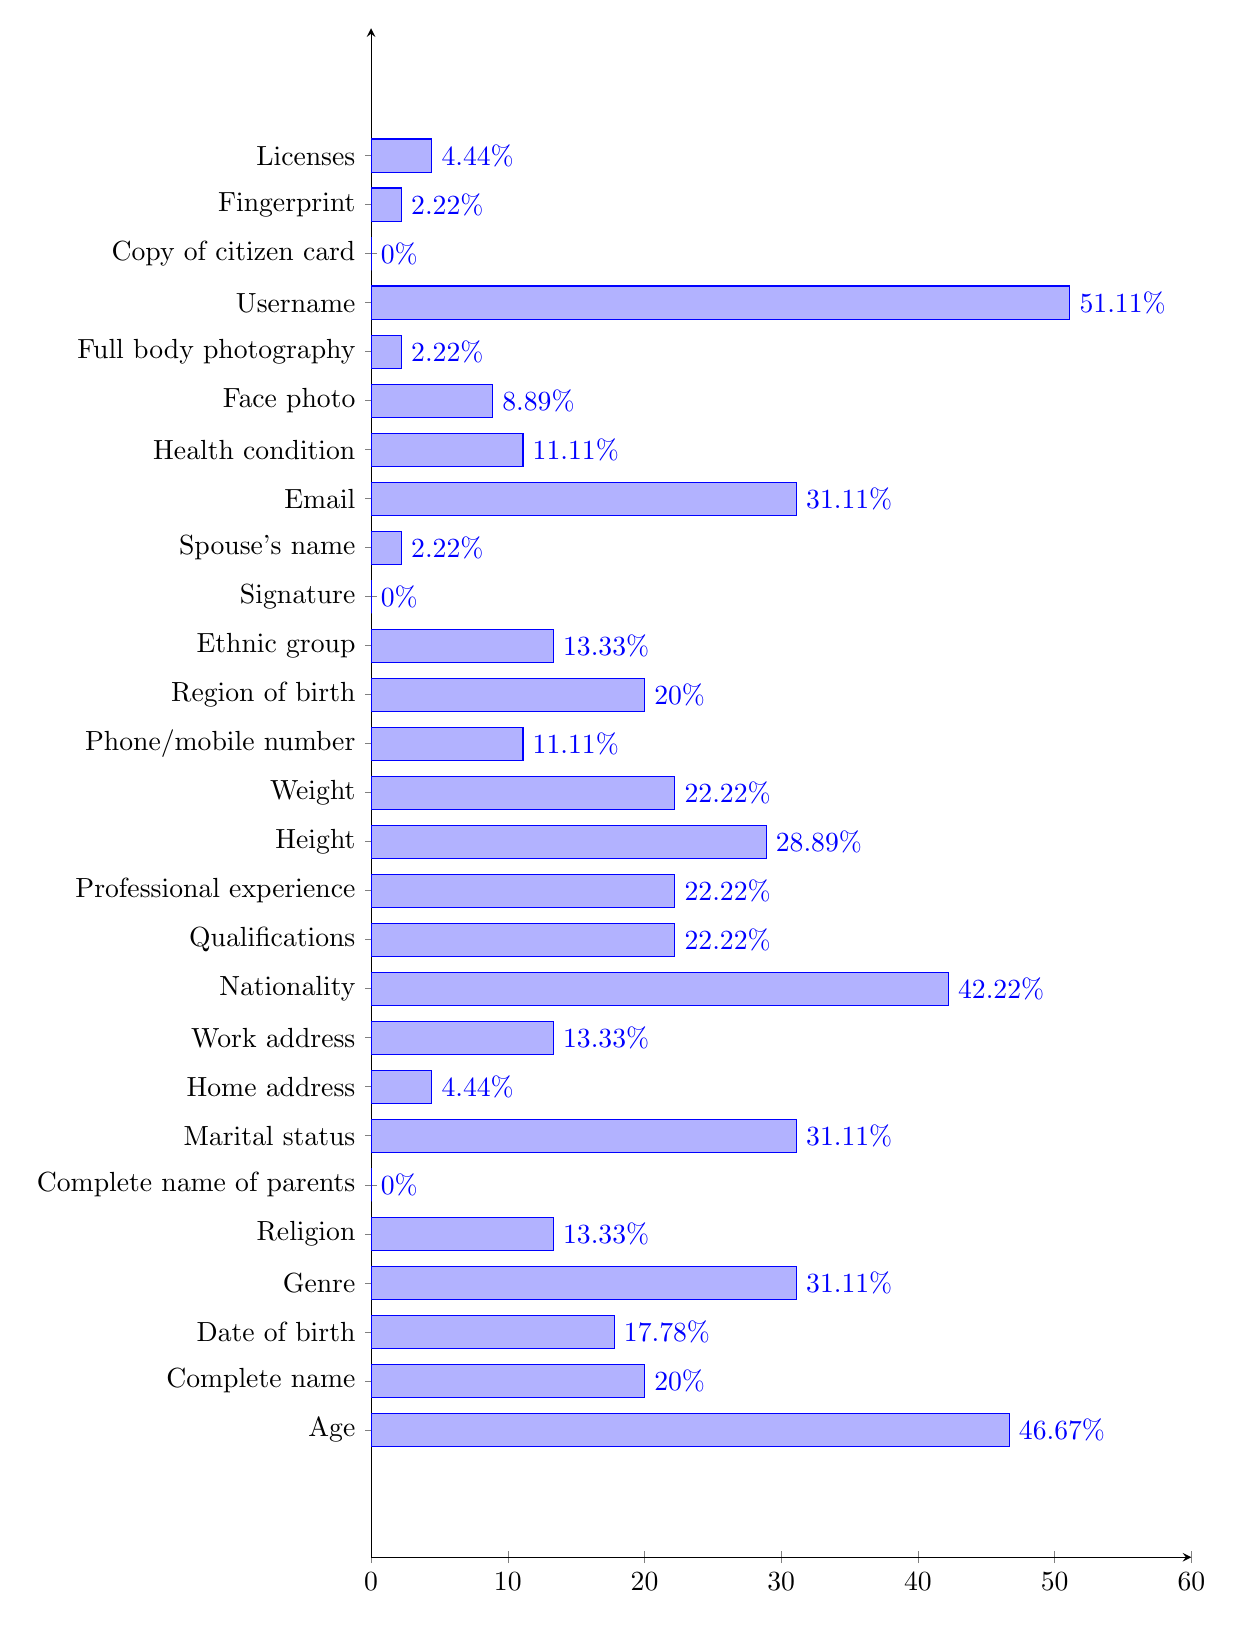
\begin{tikzpicture}
            \begin{axis}[
                height=21cm,
                width=12cm,
                xbar,
                symbolic y coords={Age,Complete name,Date of birth,Genre,Religion,Complete name of parents,Marital status,Home address,Work address,Nationality,Qualifications,Professional experience,Height,Weight,Phone/mobile number,Region of birth,Ethnic group,Signature,Spouse's name,Email,Health condition,Face photo,Full body photography,Username,Copy of citizen card,Fingerprint,Licenses},
                bar width=12pt,
                ytick=data,
                axis x line=bottom,
                axis y line=left,
                xmin=0,
                xmax=60,
                enlarge y limits=0.1,
                nodes near coords={\pgfmathprintnumber\pgfplotspointmeta\%},
            ]
                \addplot coordinates {(46.67,Age) (20,Complete name) (17.78,Date of birth) (31.11,Genre) (13.33,Religion) (0,Complete name of parents) (31.11,Marital status) (4.44,Home address) (13.33,Work address) (42.22,Nationality) (22.22,Qualifications) (22.22,Professional experience) (28.89,Height) (22.22,Weight) (11.11,Phone/mobile number) (20,Region of birth) (13.33,Ethnic group) (0,Signature) (2.22,Spouse's name) (31.11,Email) (11.11,Health condition) (8.89,Face photo) (2.22,Full body photography) (51.11,Username) (0,Copy of citizen card) (2.22,Fingerprint) (4.44,Licenses)};
            \end{axis}
        \end{tikzpicture}
        \caption*{Responses to the question: ``If you answered yes, how did you learn about the `General Data Protection Regulation' or the `California Consumer Privacy Act'?''.}
        \label{fig:survey_s2_q1}
    \end{center}
\end{figure}

2. In what situations are you willing to provide more personal information?

\begin{figure}[H]
    \begin{center}
        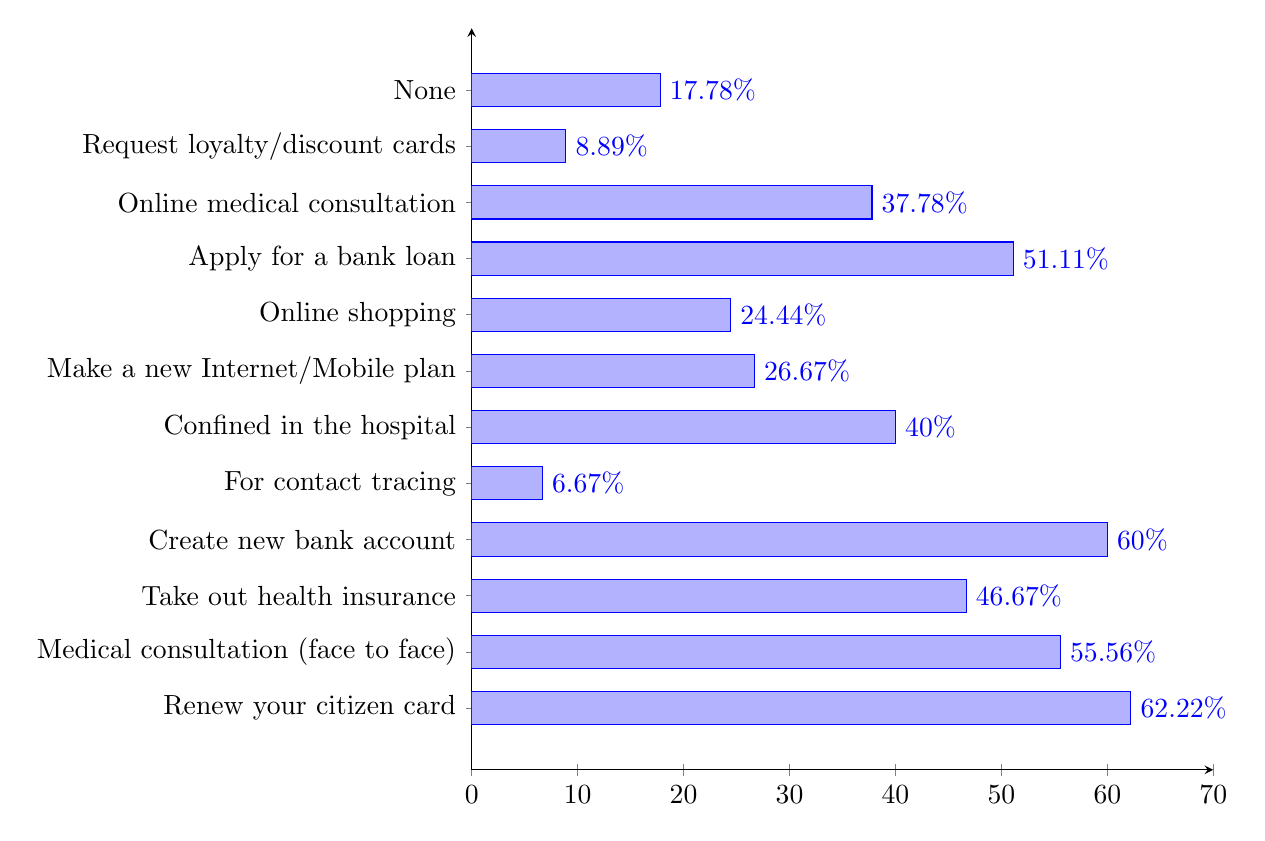
\begin{tikzpicture}
            \begin{axis}[
                height=11cm,
                width=11cm,
                xbar,
                symbolic y coords={Renew your citizen card,{Medical consultation (face to face)},Take out health insurance,Create new bank account,For contact tracing,Confined in the hospital,Make a new Internet/Mobile plan,Online shopping,Apply for a bank loan,Online medical consultation,Request loyalty/discount cards,None},
                bar width=12pt,
                ytick=data,
                axis x line=bottom,
                axis y line=left,
                xmin=0,
                xmax=70,
                enlarge y limits=0.1,
                nodes near coords={\pgfmathprintnumber\pgfplotspointmeta\%},
            ]
                \addplot coordinates {(62.22,Renew your citizen card) (55.56,{Medical consultation (face to face)}) (46.67,Take out health insurance) (60,Create new bank account) (6.67,For contact tracing) (40,Confined in the hospital) (26.67,Make a new Internet/Mobile plan) (24.44,Online shopping) (51.11,Apply for a bank loan) (37.78,Online medical consultation) (8.89,Request loyalty/discount cards) (17.78,None)};
            \end{axis}
        \end{tikzpicture}
        \caption*{Responses to the question: ``If you answered yes, how did you learn about the `General Data Protection Regulation' or the `California Consumer Privacy Act'?''.}
        \label{fig:survey_s2_q2}
    \end{center}
\end{figure}

3. Do you agree to share health data that can identify you with health professionals?

\begin{figure}[H]
    \centering
    \begin{tikzpicture}
        \pie[explode = 0.1]{4.44/I do not know,
            8.89/I disagree,
            51.11/Maybe if asked first,
            35.56/I agree}
    \end{tikzpicture}
    \caption*{Responses to the question: ``Do you agree to share health data that can identify you with health professionals?''.}
    \label{fig:survey_s2_q3}
\end{figure}

4. Do you agree to share health data that cannot identify you with health professionals?

\begin{figure}[H]
    \centering
    \begin{tikzpicture}
        \pie[explode = 0.1]{6.67/I do not know,
            17.78/I disagree,
            37.78/Maybe if asked first,
            37.78/I agree}
    \end{tikzpicture}
    \caption*{Responses to the question: ``Do you agree to share health data that cannot identify you with health professionals?''.}
    \label{fig:survey_s2_q4}
\end{figure}

5. What kind of applications do you have installed on your smartphone?

\begin{figure}[H]
    \begin{center}
        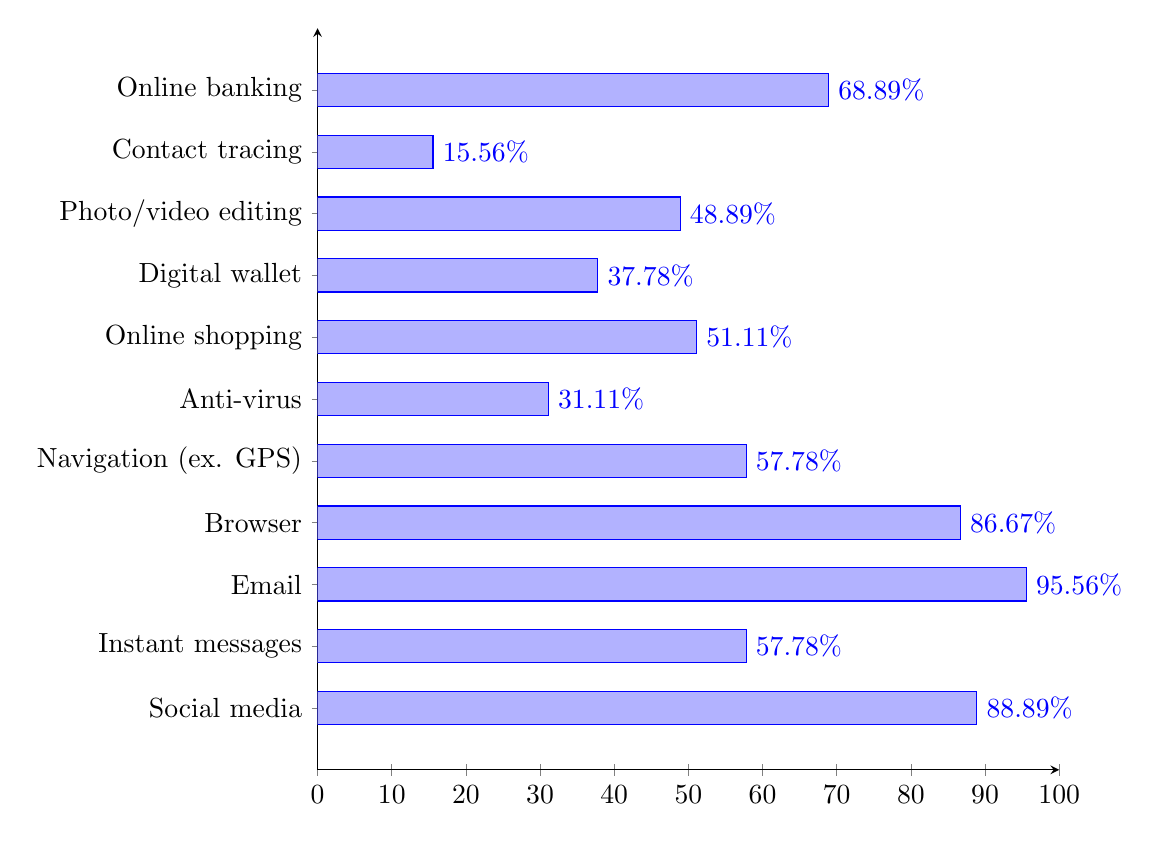
\begin{tikzpicture}
            \begin{axis}[
                height=11cm,
                width=11cm,
                xbar,
                symbolic y coords={Social media,Instant messages,Email,Browser,{Navigation (ex. GPS)},Anti-virus,Online shopping,Digital wallet,Photo/video editing,Contact tracing,Online banking},
                bar width=12pt,
                ytick=data,
                axis x line=bottom,
                axis y line=left,
                xmin=0,
                xmax=100,
                enlarge y limits=0.1,
                nodes near coords={\pgfmathprintnumber\pgfplotspointmeta\%},
            ]
                \addplot coordinates {(88.89,Social media) (57.78,Instant messages) (95.56,Email) (86.67,Browser) (57.78,{Navigation (ex. GPS)}) (31.11,Anti-virus) (51.11,Online shopping) (37.78,Digital wallet) (48.89,Photo/video editing) (15.56,Contact tracing) (68.89,Online banking)};
            \end{axis}
        \end{tikzpicture}
        \caption*{Responses to the question: ``What kind of applications do you have installed on your smartphone?''.}
        \label{fig:survey_s2_q5}
    \end{center}
\end{figure}

6. Before sharing your data, do you consult any of the following information?

\begin{figure}[H]
    \begin{center}
        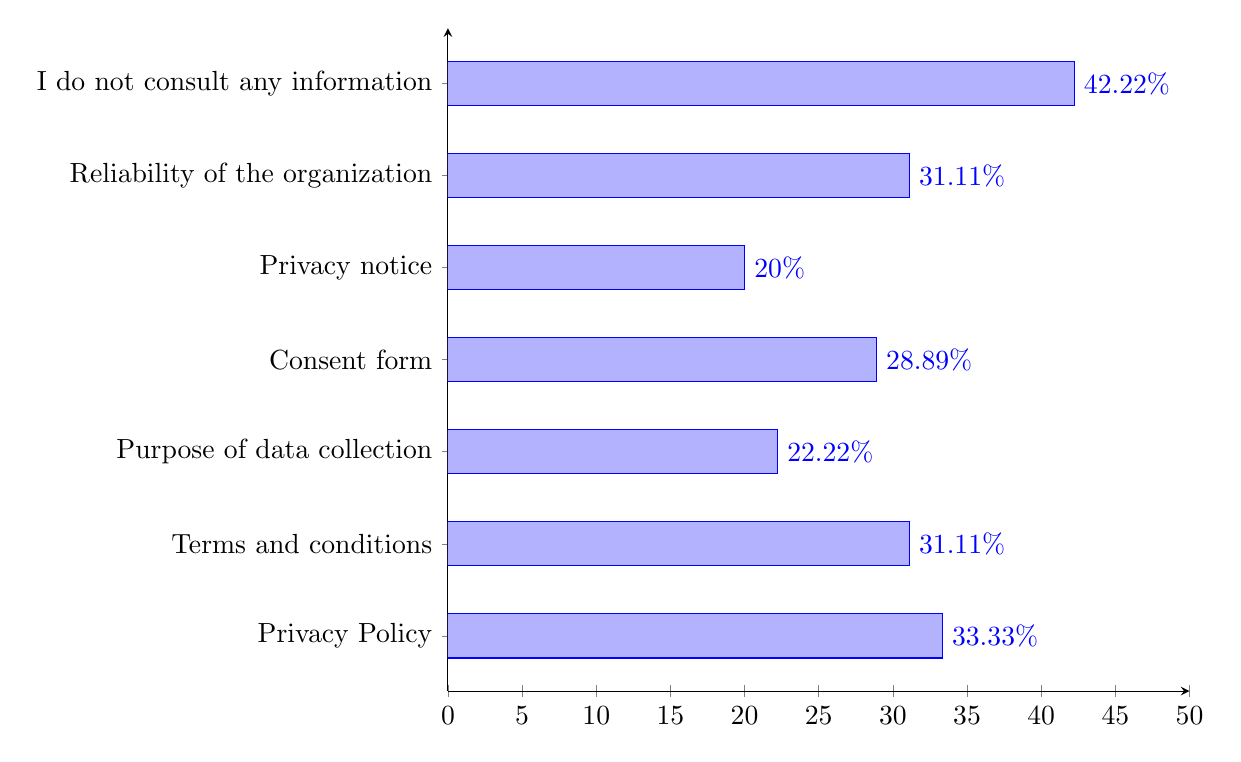
\begin{tikzpicture}
            \begin{axis}[
                height=10cm,
                width=11cm,
                xbar,
                symbolic y coords={Privacy Policy,Terms and conditions,Purpose of data collection,Consent form,Privacy notice,Reliability of the organization,I do not consult any information},
                bar width=16pt,
                ytick=data,
                axis x line=bottom,
                axis y line=left,
                xmin=0,
                xmax=50,
                enlarge y limits=0.1,
                nodes near coords={\pgfmathprintnumber\pgfplotspointmeta\%},
            ]
                \addplot coordinates {(33.33,Privacy Policy) (31.11,Terms and conditions) (22.22,Purpose of data collection) (28.89,Consent form) (20,Privacy notice) (31.11,Reliability of the organization) (42.22,I do not consult any information)};
            \end{axis}
        \end{tikzpicture}
        \caption*{Responses to the question: ``Before sharing your data, do you consult any of the following information?''.}
        \label{fig:survey_s2_q6}
    \end{center}
\end{figure}

\vspace{1cm}

7. How often do you find privacy policies?

\begin{figure}[H]
    \centering
    \begin{tikzpicture}
        \pie[explode = 0.1]{6.67/Never,
            17.78/Very rarely,
            8.89/Once a month,
            22.22/Once a week,
            44.44/Almost everyday}
    \end{tikzpicture}
    \caption*{Responses to the question: ``How often do you find privacy policies?''.}
    \label{fig:survey_s2_q7}
\end{figure}

8. Are you aware of the duties of a Data Protection Officer (DPO)?

\begin{figure}[H]
    \centering
    \begin{tikzpicture}
        \pie[explode = 0.1]{73.33/No,
            26.67/Yes}
    \end{tikzpicture}
    \caption*{Responses to the question: ``Are you aware of the duties of a Data Protection Officer (DPO)?''.}
    \label{fig:survey_s2_q8}
\end{figure}

\vspace{2cm}

9. ``I am interested in knowing where and how my personal information is used''. Do you agree with this statement?

\begin{figure}[H]
    \centering
    \begin{tikzpicture}
        \pie[explode = 0.1]{2.22/I disagree,
            15.56/I do not agree nor disagree,
            82.22/I agree}
    \end{tikzpicture}
    \caption*{Responses to the question: ```I am interested in knowing where and how my personal information is used'. Do you agree with this statement?''.}
    \label{fig:survey_s2_q9}
\end{figure}

\clearpage

10. ``I am not familiar with the purpose of data collection but would like to know more''. Do you agree with this statement?

\begin{figure}[H]
    \begin{center}
        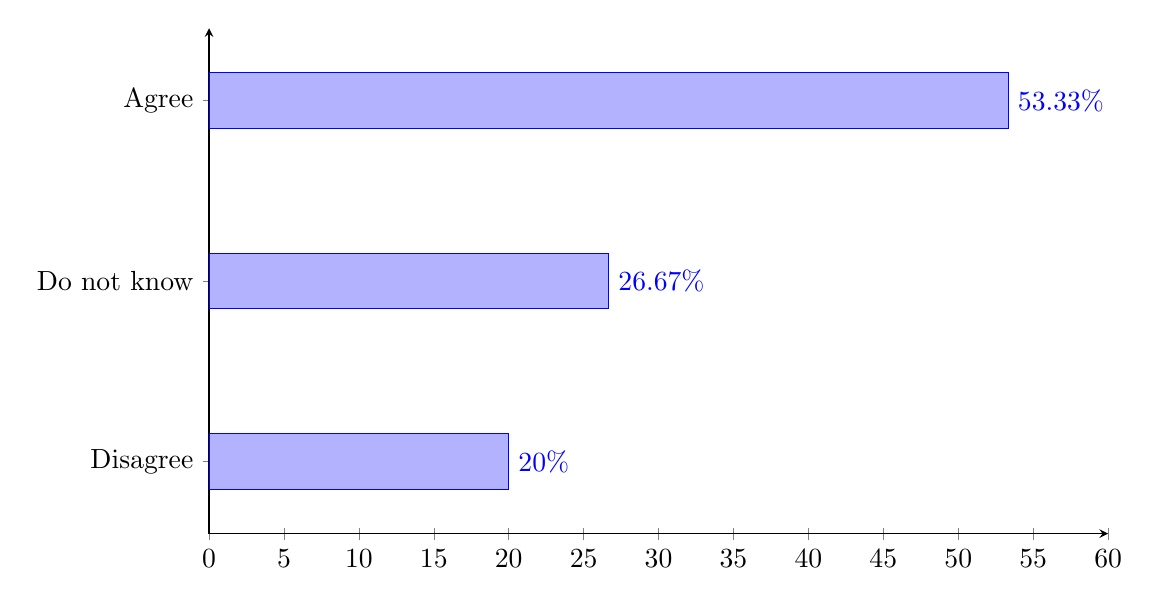
\begin{tikzpicture}
            \begin{axis}[
                height=8cm,
                width=13cm,
                xbar,
                symbolic y coords={Disagree,Do not know,Agree},
                bar width=20pt,
                ytick=data,
                axis x line=bottom,
                axis y line=left,
                xmin=0,
                xmax=60,
                enlarge y limits=0.2,
                nodes near coords={\pgfmathprintnumber\pgfplotspointmeta\%},
            ]
                \addplot coordinates {(20,Disagree) (26.67,Do not know) (53.33,Agree)};
            \end{axis}
        \end{tikzpicture}
        \caption*{Responses to the question: ```I am not familiar with the purpose of data collection but would like to know more'. Do you agree with this statement?''.}
        \label{fig:survey_s2_q10}
    \end{center}
\end{figure}

\vspace{2cm}

11. ``The length (or number of words) of the privacy notice affects my willingness to read it''. Do you agree with this statement?

\begin{figure}[H]
    \begin{center}
        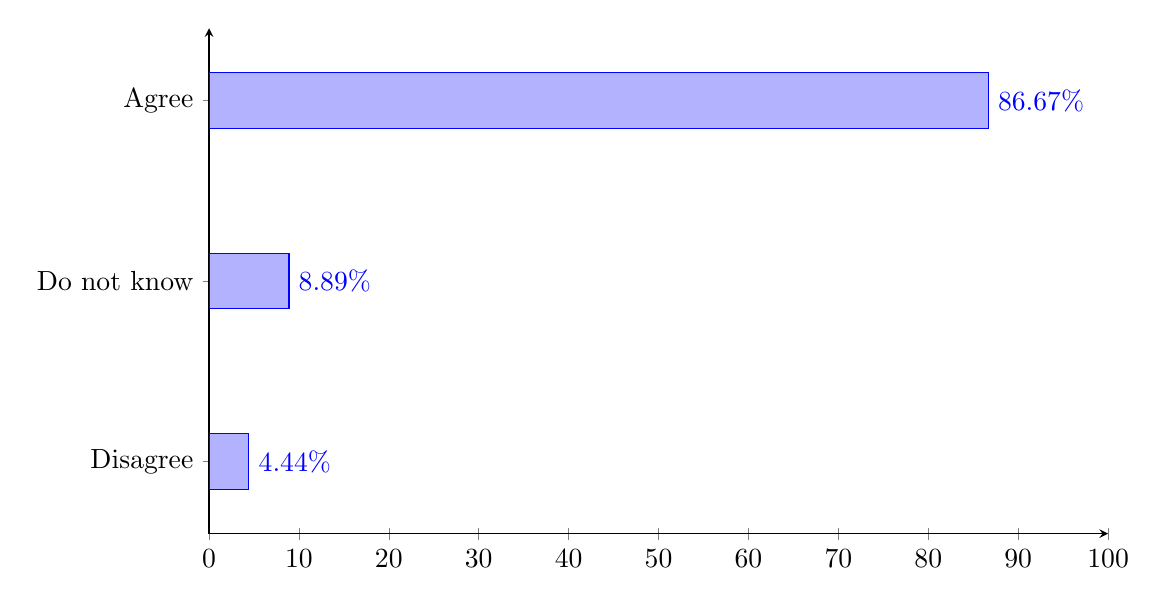
\begin{tikzpicture}
            \begin{axis}[
                height=8cm,
                width=13cm,
                xbar,
                symbolic y coords={Disagree,Do not know,Agree},
                bar width=20pt,
                ytick=data,
                axis x line=bottom,
                axis y line=left,
                xmin=0,
                xmax=100,
                enlarge y limits=0.2,
                nodes near coords={\pgfmathprintnumber\pgfplotspointmeta\%},
            ]
                \addplot coordinates {(4.44,Disagree) (8.89,Do not know) (86.67,Agree)};
            \end{axis}
        \end{tikzpicture}
        \caption*{Responses to the question: ```The length (or number of words) of the privacy notice affects my willingness to read it'. Do you agree with this statement?''.}
        \label{fig:survey_s2_q11}
    \end{center}
\end{figure}

12. ``The font size of the privacy notice affects my willingness to read it''. Do you agree with this statement?

\begin{figure}[H]
    \begin{center}
        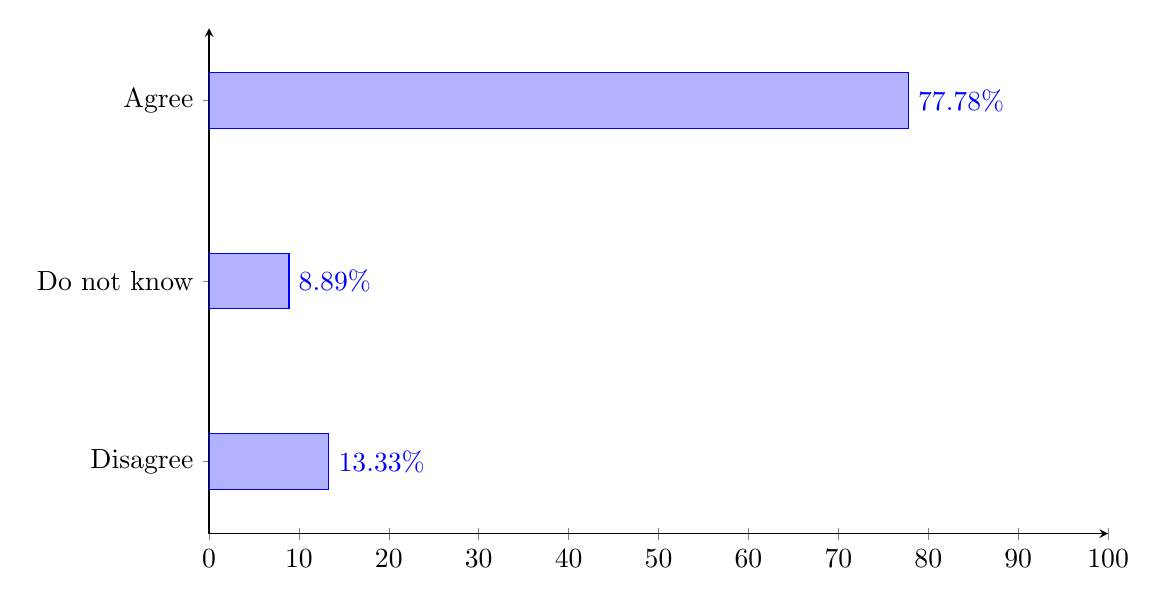
\begin{tikzpicture}
            \begin{axis}[
                height=8cm,
                width=13cm,
                xbar,
                symbolic y coords={Disagree,Do not know,Agree},
                bar width=20pt,
                ytick=data,
                axis x line=bottom,
                axis y line=left,
                xmin=0,
                xmax=100,
                enlarge y limits=0.2,
                nodes near coords={\pgfmathprintnumber\pgfplotspointmeta\%},
            ]
                \addplot coordinates {(13.33,Disagree) (8.89,Do not know) (77.78,Agree)};
            \end{axis}
        \end{tikzpicture}
        \caption*{Responses to the question: ```The font size of the privacy notice affects my willingness to read it'. Do you agree with this statement?''.}
        \label{fig:survey_s2_q12}
    \end{center}
\end{figure}

\vspace{2cm}

13. ``Usually, I'm afraid I won't be able to use a product or service if I don't agree with the privacy notice''. Do you agree with this statement?

\begin{figure}[H]
    \begin{center}
        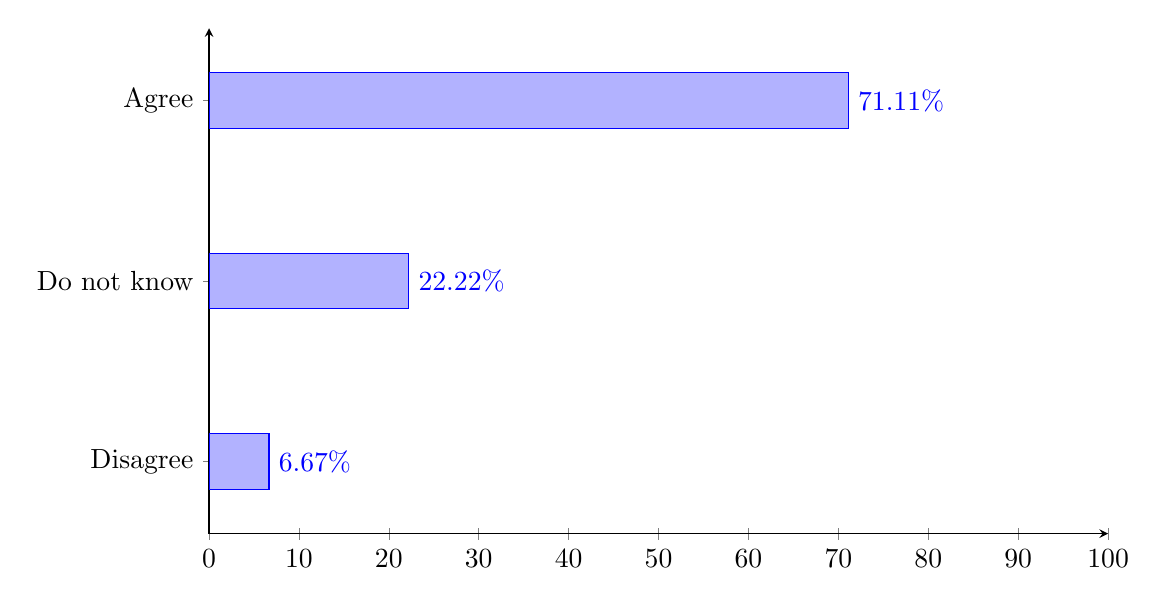
\begin{tikzpicture}
            \begin{axis}[
                height=8cm,
                width=13cm,
                xbar,
                symbolic y coords={Disagree,Do not know,Agree},
                bar width=20pt,
                ytick=data,
                axis x line=bottom,
                axis y line=left,
                xmin=0,
                xmax=100,
                enlarge y limits=0.2,
                nodes near coords={\pgfmathprintnumber\pgfplotspointmeta\%},
            ]
                \addplot coordinates {(6.67,Disagree) (22.22,Do not know) (71.11,Agree)};
            \end{axis}
        \end{tikzpicture}
        \caption*{Responses to the question: ```Usually, I'm afraid I won't be able to use a product or service if I don't agree with the privacy notice'. Do you agree with this statement?''.}
        \label{fig:survey_s2_q13}
    \end{center}
\end{figure}

14. ``I don't need to read the privacy notice if I trust the institution''. Do you agree with this statement?

\begin{figure}[H]
    \begin{center}
        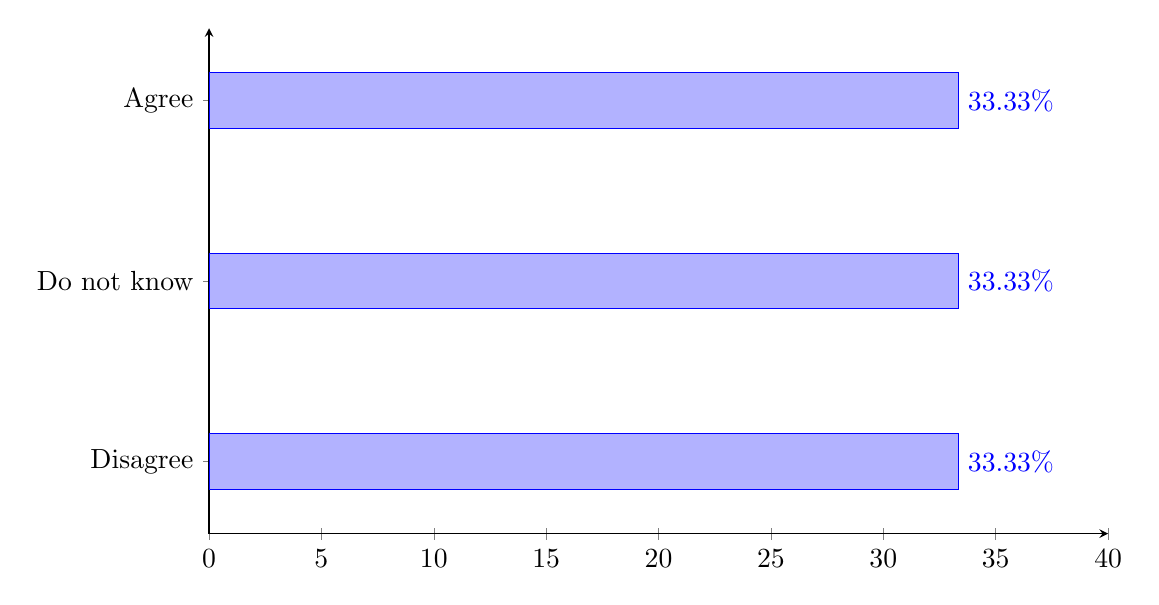
\begin{tikzpicture}
            \begin{axis}[
                height=8cm,
                width=13cm,
                xbar,
                symbolic y coords={Disagree,Do not know,Agree},
                bar width=20pt,
                ytick=data,
                axis x line=bottom,
                axis y line=left,
                xmin=0,
                xmax=40,
                enlarge y limits=0.2,
                nodes near coords={\pgfmathprintnumber\pgfplotspointmeta\%},
            ]
                \addplot coordinates {(33.33,Disagree) (33.33,Do not know) (33.33,Agree)};
            \end{axis}
        \end{tikzpicture}
        \caption*{Responses to the question: ```I don't need to read the privacy notice if I trust the institution'. Do you agree with this statement?''.}
        \label{fig:survey_s2_q14}
    \end{center}
\end{figure}

\vspace{2cm}

\subsection*{Section 3: Privacy concerns}

1. How concerned are you about organizations collecting and using your online activity?

\begin{figure}[H]
    \begin{center}
        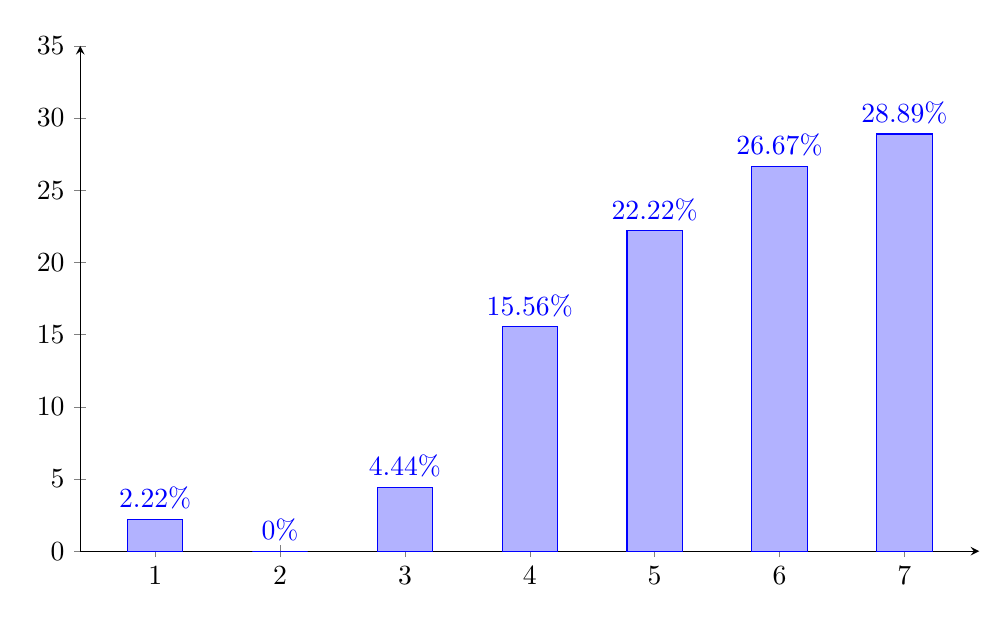
\begin{tikzpicture}
            \begin{axis}[
                height=8cm,
                width=13cm,
                ybar,
                bar width=20pt,
                ymin=0,
                ymax=35,
                xtick=data,
                axis x line=bottom,
                axis y line=left,
                enlarge x limits=0.1,
                nodes near coords={\pgfmathprintnumber\pgfplotspointmeta\%},
            ]
                \addplot coordinates {(1,2.22) (2,0) (3,4.44) (4,15.56) (5,22.22) (6,26.67) (7,28.89)};
            \end{axis}
        \end{tikzpicture}
        \caption*{Responses to the question: ``How concerned are you about organizations collecting and using your online activity?''.}
        \label{fig:survey_s3_q1}
    \end{center}
\end{figure}

2. How concerned are you about organizations sharing your data with third parties?

\begin{figure}[H]
    \begin{center}
        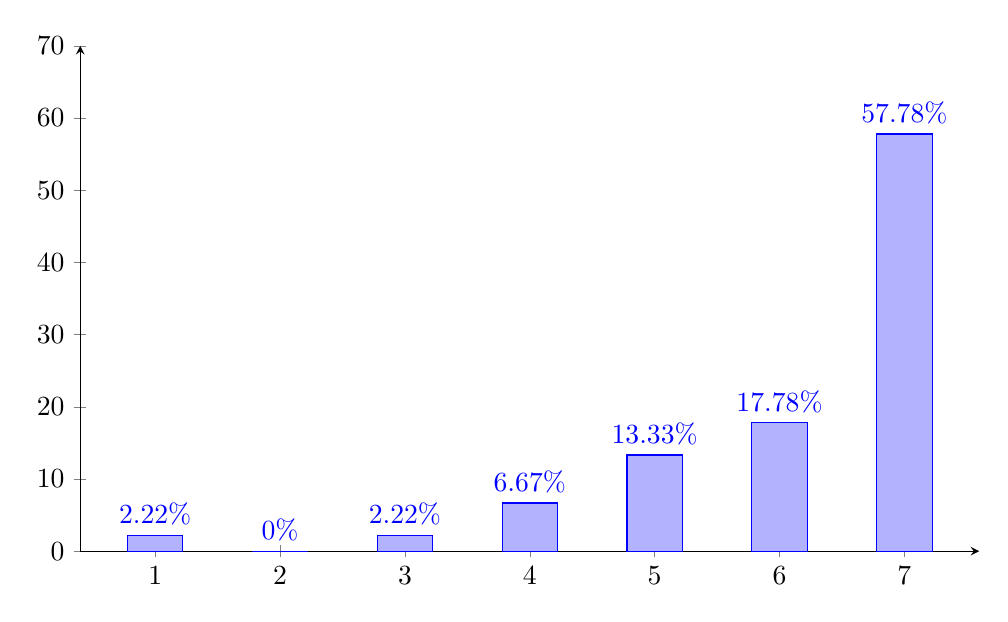
\begin{tikzpicture}
            \begin{axis}[
                height=8cm,
                width=13cm,
                ybar,
                bar width=20pt,
                ymin=0,
                ymax=70,
                xtick=data,
                axis x line=bottom,
                axis y line=left,
                enlarge x limits=0.1,
                nodes near coords={\pgfmathprintnumber\pgfplotspointmeta\%},
            ]
                \addplot coordinates {(1,2.22) (2,0) (3,2.22) (4,6.67) (5,13.33) (6,17.78) (7,57.78)};
            \end{axis}
        \end{tikzpicture}
        \caption*{Responses to the question: ``How concerned are you about organizations sharing your data with third parties?''.}
        \label{fig:survey_s3_q2}
    \end{center}
\end{figure}

\vspace{2cm}

3. How concerned are you about organizations tracking your online behavior and thus obtaining your personal data?

\begin{figure}[H]
    \begin{center}
        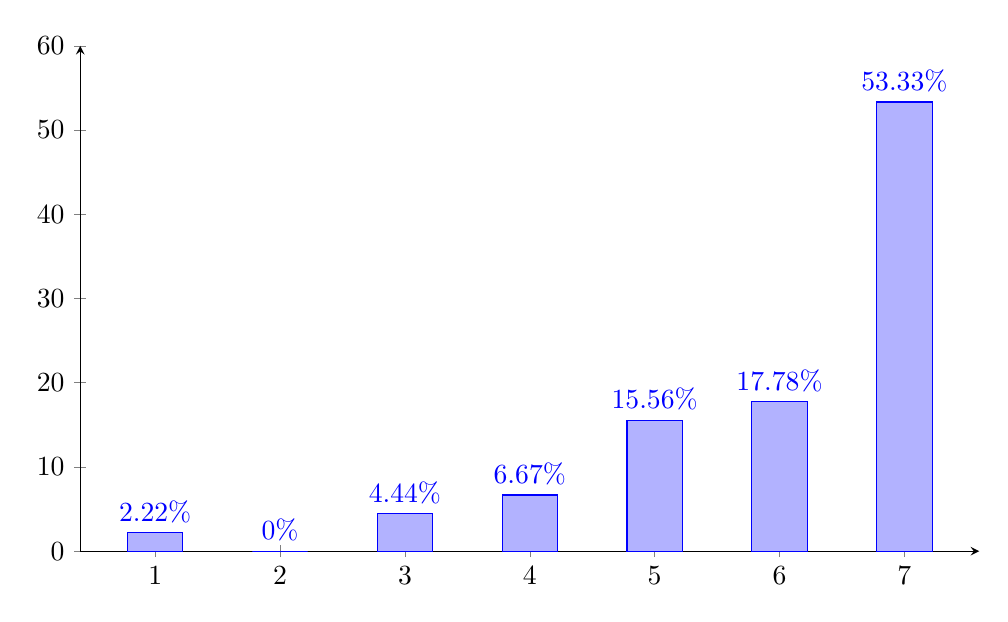
\begin{tikzpicture}
            \begin{axis}[
                height=8cm,
                width=13cm,
                ybar,
                bar width=20pt,
                ymin=0,
                ymax=60,
                xtick=data,
                axis x line=bottom,
                axis y line=left,
                enlarge x limits=0.1,
                nodes near coords={\pgfmathprintnumber\pgfplotspointmeta\%},
            ]
                \addplot coordinates {(1,2.22) (2,0) (3,4.44) (4,6.67) (5,15.56) (6,17.78) (7,53.33)};
            \end{axis}
        \end{tikzpicture}
        \caption*{Responses to the question: ``How concerned are you about organizations tracking your online behavior and thus obtaining your personal data?''.}
        \label{fig:survey_s3_q3}
    \end{center}
\end{figure}

4. How concerned are you about public institutions or intelligence services analyzing your online movements?

\begin{figure}[H]
    \begin{center}
        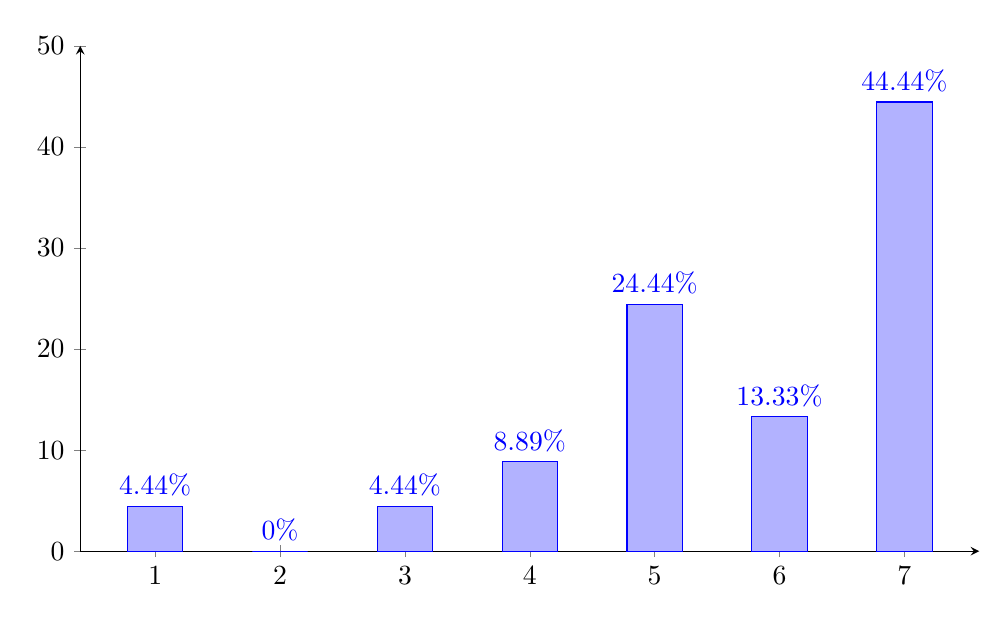
\begin{tikzpicture}
            \begin{axis}[
                height=8cm,
                width=13cm,
                ybar,
                bar width=20pt,
                ymin=0,
                ymax=50,
                xtick=data,
                axis x line=bottom,
                axis y line=left,
                enlarge x limits=0.1,
                nodes near coords={\pgfmathprintnumber\pgfplotspointmeta\%},
            ]
                \addplot coordinates {(1,4.44) (2,0) (3,4.44) (4,8.89) (5,24.44) (6,13.33) (7,44.44)};
            \end{axis}
        \end{tikzpicture}
        \caption*{Responses to the question: ``How concerned are you about public institutions or intelligence services analyzing your online movements?''.}
        \label{fig:survey_s3_q4}
    \end{center}
\end{figure}

\vspace{2cm}

5. How concerned are you that other people obtain your personal data without your consent?

\begin{figure}[H]
    \begin{center}
        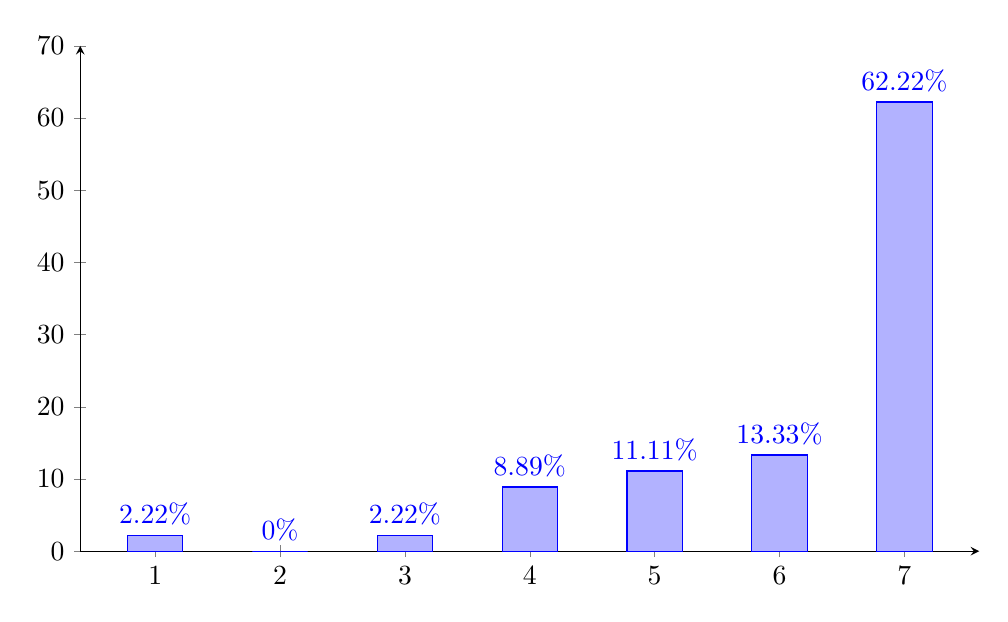
\begin{tikzpicture}
            \begin{axis}[
                height=8cm,
                width=13cm,
                ybar,
                bar width=20pt,
                ymin=0,
                ymax=70,
                xtick=data,
                axis x line=bottom,
                axis y line=left,
                enlarge x limits=0.1,
                nodes near coords={\pgfmathprintnumber\pgfplotspointmeta\%},
            ]
                \addplot coordinates {(1,2.22) (2,0) (3,2.22) (4,8.89) (5,11.11) (6,13.33) (7,62.22)};
            \end{axis}
        \end{tikzpicture}
        \caption*{Responses to the question: ``How concerned are you that other people obtain your personal data without your consent?''.}
        \label{fig:survey_s3_q5}
    \end{center}
\end{figure}

6. How concerned are you that other people find information about you online?

\begin{figure}[H]
    \begin{center}
        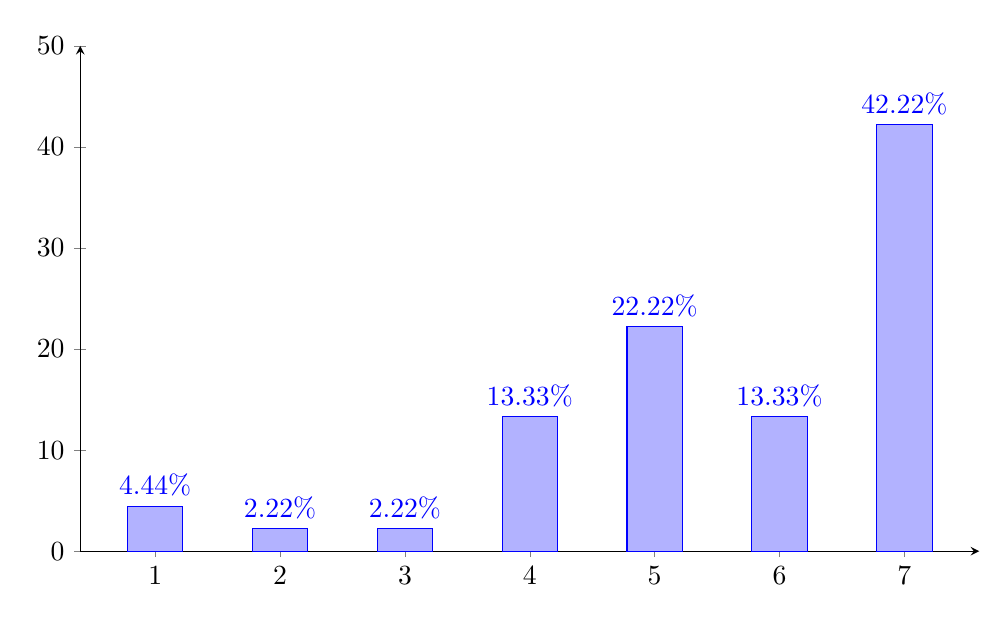
\begin{tikzpicture}
            \begin{axis}[
                height=8cm,
                width=13cm,
                ybar,
                bar width=20pt,
                ymin=0,
                ymax=50,
                xtick=data,
                axis x line=bottom,
                axis y line=left,
                enlarge x limits=0.1,
                nodes near coords={\pgfmathprintnumber\pgfplotspointmeta\%},
            ]
                \addplot coordinates {(1,4.44) (2,2.22) (3,2.22) (4,13.33) (5,22.22) (6,13.33) (7,42.22)};
            \end{axis}
        \end{tikzpicture}
        \caption*{Responses to the question: ``How concerned are you that other people find information about you online?''.}
        \label{fig:survey_s3_q6}
    \end{center}
\end{figure}

\vspace{2cm}

7. How concerned are you that other people are disclosing information about you without your knowledge?

\begin{figure}[H]
    \begin{center}
        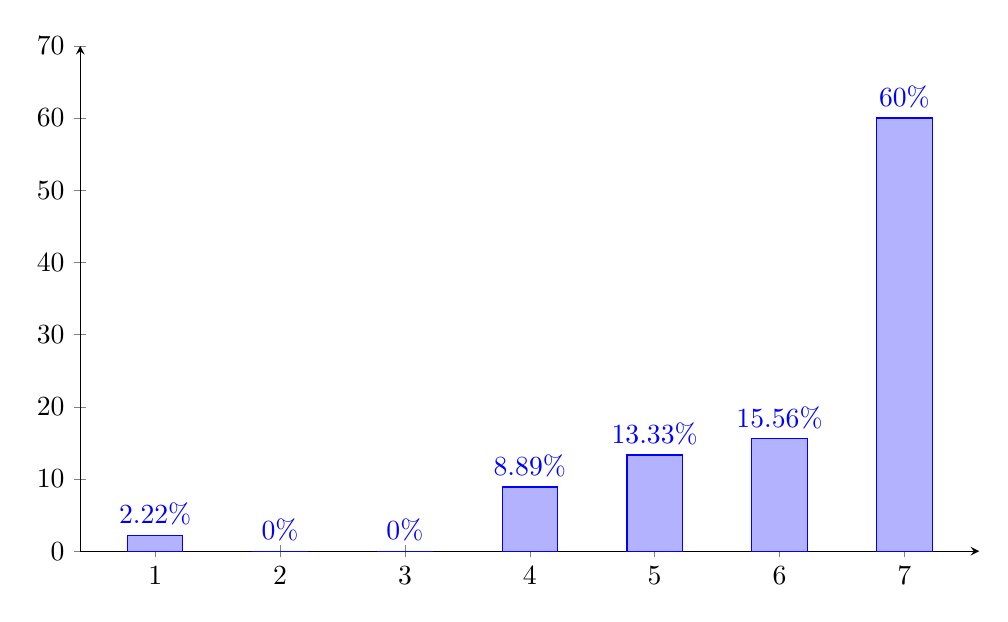
\begin{tikzpicture}
            \begin{axis}[
                height=8cm,
                width=13cm,
                ybar,
                bar width=20pt,
                ymin=0,
                ymax=70,
                xtick=data,
                axis x line=bottom,
                axis y line=left,
                enlarge x limits=0.1,
                nodes near coords={\pgfmathprintnumber\pgfplotspointmeta\%},
            ]
                \addplot coordinates {(1,2.22) (2,0) (3,0) (4,8.89) (5,13.33) (6,15.56) (7,60)};
            \end{axis}
        \end{tikzpicture}
        \caption*{Responses to the question: ``How concerned are you that other people are disclosing information about you without your knowledge?''.}
        \label{fig:survey_s3_q7}
    \end{center}
\end{figure}

8. How concerned are you about other people sharing your personal data (photos, address, mobile phone number, etc.) with others without your consent?

\begin{figure}[H]
    \begin{center}
        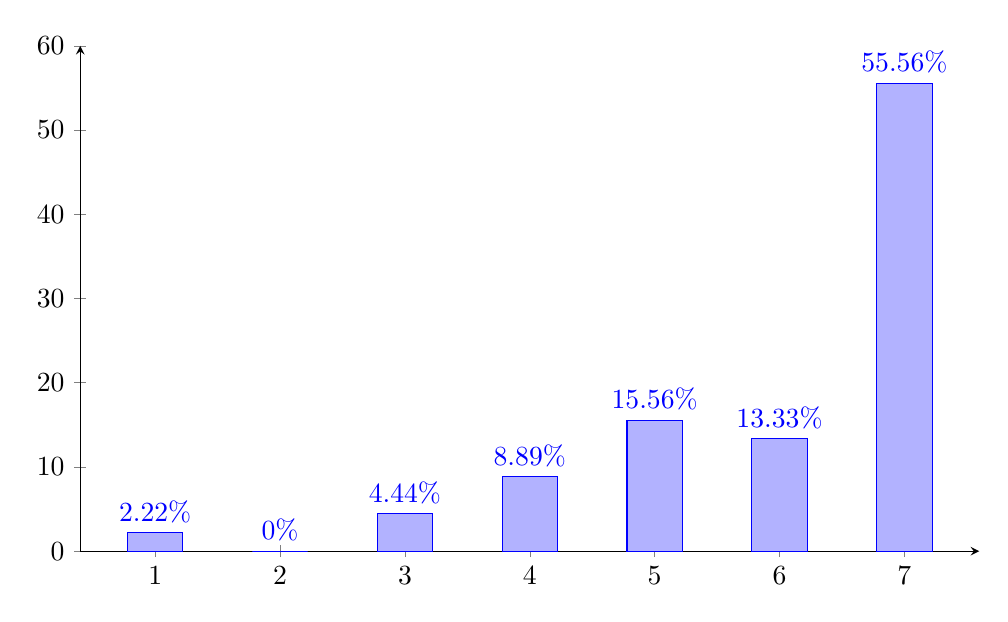
\begin{tikzpicture}
            \begin{axis}[
                height=8cm,
                width=13cm,
                ybar,
                bar width=20pt,
                ymin=0,
                ymax=60,
                xtick=data,
                axis x line=bottom,
                axis y line=left,
                enlarge x limits=0.1,
                nodes near coords={\pgfmathprintnumber\pgfplotspointmeta\%},
            ]
                \addplot coordinates {(1,2.22) (2,0) (3,4.44) (4,8.89) (5,15.56) (6,13.33) (7,55.56)};
            \end{axis}
        \end{tikzpicture}
        \caption*{Responses to the question: ``How concerned are you about other people sharing your personal data (photos, address, mobile phone number, etc.) with others without your consent?''.}
        \label{fig:survey_s3_q8}
    \end{center}
\end{figure}

\vspace{2cm}

9. How concerned are you that other people publish your personal data (photos, address, mobile phone number, etc.) on the internet without your consent?

\begin{figure}[H]
    \begin{center}
        \begin{tikzpicture}
            \begin{axis}[
                height=8cm,
                width=13cm,
                ybar,
                bar width=20pt,
                ymin=0,
                ymax=80,
                xtick=data,
                axis x line=bottom,
                axis y line=left,
                enlarge x limits=0.1,
                nodes near coords={\pgfmathprintnumber\pgfplotspointmeta\%},
            ]
                \addplot coordinates {(1,2.22) (2,0) (3,0) (4,11.11) (5,11.11) (6,2.22) (7,73.33)};
            \end{axis}
        \end{tikzpicture}
        \caption*{Responses to the question: ``How concerned are you that other people publish your personal data (photos, address, mobile phone number, etc.) on the internet without your consent?''.}
        \label{fig:survey_s3_q9}
    \end{center}
\end{figure}

10. How concerned are you about an unknown person claiming to be you on the internet?

\begin{figure}[H]
    \begin{center}
        \begin{tikzpicture}
            \begin{axis}[
                height=8cm,
                width=13cm,
                ybar,
                bar width=20pt,
                ymin=0,
                ymax=70,
                xtick=data,
                axis x line=bottom,
                axis y line=left,
                enlarge x limits=0.1,
                nodes near coords={\pgfmathprintnumber\pgfplotspointmeta\%},
            ]
                \addplot coordinates {(1,4.44) (2,4.44) (3,6.67) (4,8.89) (5,8.89) (6,6.67) (7,60)};
            \end{axis}
        \end{tikzpicture}
        \caption*{Responses to the question: ``How concerned are you about an unknown person claiming to be you on the internet?''.}
        \label{fig:survey_s3_q10}
    \end{center}
\end{figure}

\vspace{2cm}

11. How concerned are you about the possibility that someone may misuse your identity on the internet?

\begin{figure}[H]
    \begin{center}
        \begin{tikzpicture}
            \begin{axis}[
                height=8cm,
                width=13cm,
                ybar,
                bar width=20pt,
                ymin=0,
                ymax=70,
                xtick=data,
                axis x line=bottom,
                axis y line=left,
                enlarge x limits=0.1,
                nodes near coords={\pgfmathprintnumber\pgfplotspointmeta\%},
            ]
                \addplot coordinates {(1,2.22) (2,4.44) (3,2.22) (4,8.89) (5,6.67) (6,11.11) (7,64.44)};
            \end{axis}
        \end{tikzpicture}
        \caption*{Responses to the question: ``How concerned are you about the possibility that someone may misuse your identity on the internet?''.}
        \label{fig:survey_s3_q11}
    \end{center}
\end{figure}

\subsection*{Section 4: Current online habits and practices}

1. Do you have internet access at home?

\begin{figure}[H]
    \begin{center}
        \begin{tikzpicture}
            \begin{axis}[
                height=8cm,
                width=11cm,
                xbar,
                symbolic y coords={By WiFi or Ethernet cable,By mobile network,No},
                bar width=20pt,
                ytick=data,
                axis x line=bottom,
                axis y line=left,
                xmin=0,
                xmax=100,
                enlarge y limits=0.2,
                nodes near coords={\pgfmathprintnumber\pgfplotspointmeta\%},
            ]
                \addplot coordinates {(93.33,By WiFi or Ethernet cable) (64.44,By mobile network) (0,No)};
            \end{axis}
        \end{tikzpicture}
        \caption*{Responses to the question: ``Do you have internet access at home?''.}
        \label{fig:survey_s4_q1}
    \end{center}
\end{figure}

\vspace{2cm}

2. How often do you use the internet?\\

\begin{figure}[H]
    \centering
    \begin{tikzpicture}
        \pie[explode = 0.1]{0/Never,
            0/Once a month,
            0/Once a week,
            4.44/2 or 3 days a week,
            95.56/Everyday}
    \end{tikzpicture}
    \caption*{Responses to the question: ``How often do you use the internet?''.}
    \label{fig:survey_s4_q2}
\end{figure}

\clearpage

3. How much time do you spend per day surfing the internet?

\begin{figure}[H]
    \centering
    \begin{tikzpicture}
        \pie[explode = 0.1]{13.33/10+ hours,
            26.67/5-10 hours,
            42.22/2-5 hours,
            15.56/1-2 hours,
            2.22/<1 hour}
    \end{tikzpicture}
    \caption*{Responses to the question: ``How much time do you spend per day surfing the internet?''.}
    \label{fig:survey_s4_q3}
\end{figure}

\vspace{2cm}

4. What device(s) do you use to access the internet?

\begin{figure}[H]
    \begin{center}
        \begin{tikzpicture}
            \begin{axis}[
                height=10cm,
                width=11cm,
                xbar,
                symbolic y coords={Computer,Portable computer,Tablet,Phone},
                bar width=20pt,
                ytick=data,
                axis x line=bottom,
                axis y line=left,
                xmin=0,
                xmax=100,
                enlarge y limits=0.2,
                nodes near coords={\pgfmathprintnumber\pgfplotspointmeta\%},
            ]
                \addplot coordinates {(51.11,Computer) (75.56,Portable computer) (26.67,Tablet) (95.56,Phone)};
            \end{axis}
        \end{tikzpicture}
        \caption*{Responses to the question: ``What device(s) do you use to access the internet?''.}
        \label{fig:survey_s4_q4}
    \end{center}
\end{figure}

5. For what purposes do you use the internet?

\begin{figure}[H]
    \begin{center}
        \begin{tikzpicture}
            \begin{axis}[
                height=11cm,
                width=10cm,
                xbar,
                symbolic y coords={{Search for information about politics, health, etc.},Social media,Online shopping,Consult email,Listen to music,Play videogames,Watch movies/series,Study online,Look for a job,Work,Publish to a blog or online journal},
                bar width=12pt,
                ytick=data,
                yticklabels={
                    {Search for information about\\politics, health, etc.},
                    Social media,
                    Online shopping,
                    Consult email,
                    Listen to music,
                    Play videogames,
                    Watch movies/series,
                    Study online,
                    Look for a job,
                    Work,
                    Publish to a blog\\or online journal
                },
                yticklabel style={align=right},
                axis x line=bottom,
                axis y line=left,
                xmin=0,
                xmax=100,
                enlarge y limits=0.2,
                nodes near coords={\pgfmathprintnumber\pgfplotspointmeta\%},
            ]
                \addplot coordinates {(73.33,{Search for information about politics, health, etc.}) (80,Social media) (66.67,Online shopping) (84.44,Consult email) (82.22,Listen to music) (46.67,Play videogames) (75.56,Watch movies/series) (77.78,Study online) (42.22,Look for a job) (62.22,Work) (6.67,Publish to a blog or online journal)};
            \end{axis}
        \end{tikzpicture}
        \caption*{Responses to the question: ``For what purposes do you use the internet?''.}
        \label{fig:survey_s4_q5}
    \end{center}
\end{figure}

6. What platforms/applications do you use in your day-to-day life?

\begin{figure}[H]
    \begin{center}
        \begin{tikzpicture}
            \begin{axis}[
                height=10cm,
                width=11cm,
                xbar,
                symbolic y coords={Social media,Instant messages,Email,Browser,Online shopping,Photo/video editing,Online banking,Anti-virus,Contact tracing,Delivery services},
                bar width=12pt,
                ytick=data,
                axis x line=bottom,
                axis y line=left,
                xmin=0,
                xmax=100,
                enlarge y limits=0.1,
                nodes near coords={\pgfmathprintnumber\pgfplotspointmeta\%},
            ]
                \addplot coordinates {(80,Social media) (68.89,Instant messages) (88.89,Email) (82.22,Browser) (51.11,Online shopping) (26.67,Photo/video editing) (55.56,Online banking) (15.56,Anti-virus) (0,Contact tracing) (31.11,Delivery services)};
            \end{axis}
        \end{tikzpicture}
        \caption*{Responses to the question: ``What platforms/applications do you use in your day-to-day life?''.}
        \label{fig:survey_s4_q6}
    \end{center}
\end{figure}

7. On social media, do you usually:

\begin{figure}[H]
    \begin{center}
        \begin{tikzpicture}
            \begin{axis}[
                height=8cm,
                width=11cm,
                xbar,
                symbolic y coords={Use your own photo showing your face as your profile picture,Use your real and full name,{Put the date of birth, age and other information},Do not post information that could identify me},
                bar width=20pt,
                ytick=data,
                yticklabels={
                    Use your own photo showing your\\face as your profile picture,
                    Use your real and full name,
                    {Put the date of birth, age\\and other information},
                    Do not post information that\\could identify me,
                },
                yticklabel style={align=right},
                axis x line=bottom,
                axis y line=left,
                xmin=0,
                xmax=80,
                enlarge y limits=0.1,
                nodes near coords={\pgfmathprintnumber\pgfplotspointmeta\%},
            ]
                \addplot coordinates {(66.67,Use your own photo showing your face as your profile picture) (44.44,Use your real and full name) (35.56,{Put the date of birth, age and other information}) (26.67,Do not post information that could identify me)};
            \end{axis}
        \end{tikzpicture}
        \caption*{Responses to the question: ``On social media, do you usually:''.}
        \label{fig:survey_s4_q7}
    \end{center}
\end{figure}

8. Your activity on social media goes through:

\begin{figure}[H]
    \begin{center}
        \begin{tikzpicture}
            \begin{axis}[
                height=12cm,
                width=11cm,
                xbar,
                symbolic y coords={Sharing photos of children/family members who are minors,{Follow any elected officials, candidates for office or other political figures},{Follow celebrities, or people with some notoriety},{Post links to/from business, sport or articles},Post links to political stories or other articles,Post political or social opinions,I don't use social media},
                bar width=18pt,
                ytick=data,
                yticklabels={
                    Sharing photos of children/family\\members who are minors,
                    {Follow any elected officials, candidates\\for office or other political figures},
                    {Follow celebrities, or\\people with some notoriety},
                    {Post links to/from business,\\sport or articles},
                    Post links to political stories\\or other articles,
                    Post political or\\social opinions,
                    I don't use social media,
                },
                yticklabel style={align=right},
                axis x line=bottom,
                axis y line=left,
                xmin=0,
                xmax=60,
                enlarge y limits=0.1,
                nodes near coords={\pgfmathprintnumber\pgfplotspointmeta\%},
            ]
                \addplot coordinates {(8.89,Sharing photos of children/family members who are minors) (22.22,{Follow any elected officials, candidates for office or other political figures}) (55.56,{Follow celebrities, or people with some notoriety}) (24.44,{Post links to/from business, sport or articles}) (13.33,Post links to political stories or other articles) (15.56,Post political or social opinions) (26.67,I don't use social media)};
            \end{axis}
        \end{tikzpicture}
        \caption*{Responses to the question: ``Your activity on social media goes through:''.}
        \label{fig:survey_s4_q8}
    \end{center}
\end{figure}

\subsection*{Section 5: Profile identification}

1. Do you know the concept of profiling?

\begin{table}[H]
    \centering
    \begin{tabular}{p{3cm} p{12cm}}
        \hline
        \textbf{Participant} & \textbf{Answer} \\
        \hline
        P1 & ``É aquele que estuda e analisa o comportamento de um indivíduo e os seus habitos'' \\
        \hline
        P2 & ``Reunir informações sobre um indivíduo de modo a poder caracteriza-lo.'' \\
        \hline
        P3 & ``Estudo do perfil online'' \\
        \hline
        P4 & ``Ideia geral de quem e a pessoa o que faz o qie gosta onde e quando vai a algum lugar quem sao amigos familiares etc'' \\
        \hline
        P5 & ``Identificar o perfil comportamental de uma pessoa, com base nas suas informações pessais'' \\
        \hline
        P6 & ``É quando uma empresa ou alguém forma um perfil da nossa identidade com a informação recolhida online'' \\
        \hline
        P7 & ``estratégia de marketing que ajuda a identificar clientes'' \\
        \hline
        P8 & ``É a criação de um perfil de utilizador consoante os seus interesses.'' \\
        \hline
        P9 & ``Prejudgement of a person based on the way they look (informed by social norms)'' \\
        \hline
        P10 & ``Somewhat, I think I know what it entails but couldn't name a perfect definition'' \\
        \hline
        P11 & ``Profiling is when companies collect data about us in order to improve their advertising. '' \\
        \hline
        P12 & ``Making a profile for a person based on their internet activity or something like that maybe'' \\
        \hline
        P13-P20 & Yes but do not know how to explain \\
        \hline
        P20-P45 & Do not know \\
        \hline
    \end{tabular}
    \vspace{1em}
    \caption*{Responses to the question: ``What do you understand by Internet of Things?''.}
    \label{table:survey_s5_q1}
\end{table}

2. If a law enforcement officer asks for your personal data, are you willing to share it?

\begin{figure}[H]
    \centering
    \begin{tikzpicture}
        \pie[explode = 0.1]{35.56/I do not know,
            11.11/No,
            53.33/Yes}
    \end{tikzpicture}
    \caption*{Responses to the question: ``If a law enforcement officer asks for your personal data, are you willing to share it?''.}
    \label{fig:survey_s5_q2}
\end{figure}

3. In what situations are you willing to provide personal data when data collection is disclosed?

\begin{figure}[H]
    \begin{center}
        \begin{tikzpicture}
            \begin{axis}[
                height=9.5cm,
                width=11cm,
                xbar,
                symbolic y coords={Renew your citizen card,{Medical consultation (face to face)},Take out health insurance,Create new bank account,For contact tracing,Confined in the hospital,Make a new Internet/Mobile plan,Online shopping,Apply for a bank loan,Online medical consultation,Request loyalty/discount cards,None},
                bar width=12pt,
                ytick=data,
                axis x line=bottom,
                axis y line=left,
                xmin=0,
                xmax=70,
                enlarge y limits=0.1,
                nodes near coords={\pgfmathprintnumber\pgfplotspointmeta\%},
            ]
                \addplot coordinates {(55.56,Renew your citizen card) (48.89,{Medical consultation (face to face)}) (31.11,Take out health insurance) (55.56,Create new bank account) (2.22,For contact tracing) (44.44,Confined in the hospital) (24.44,Make a new Internet/Mobile plan) (22.22,Online shopping) (37.78,Apply for a bank loan) (22.22,Online medical consultation) (6.67,Request loyalty/discount cards) (24.44,None)};
            \end{axis}
        \end{tikzpicture}
        \caption*{Responses to the question: ``In what situations are you willing to provide personal data when data collection is disclosed?''.}
        \label{fig:survey_s5_q3}
    \end{center}
\end{figure}

4. In what situations are you willing to provide personal data when data collection is not disclosed?

\begin{figure}[H]
    \begin{center}
        \begin{tikzpicture}
            \begin{axis}[
                height=9.5cm,
                width=11cm,
                xbar,
                symbolic y coords={Renew your citizen card,{Medical consultation (face to face)},Take out health insurance,Create new bank account,For contact tracing,Confined in the hospital,Make a new Internet/Mobile plan,Online shopping,Apply for a bank loan,Online medical consultation,Request loyalty/discount cards,None},
                bar width=12pt,
                ytick=data,
                axis x line=bottom,
                axis y line=left,
                xmin=0,
                xmax=70,
                enlarge y limits=0.1,
                nodes near coords={\pgfmathprintnumber\pgfplotspointmeta\%},
            ]
                \addplot coordinates {(44.44,Renew your citizen card) (53.33,{Medical consultation (face to face)}) (26.67,Take out health insurance) (37.78,Create new bank account) (11.11,For contact tracing) (26.67,Confined in the hospital) (20,Make a new Internet/Mobile plan) (28.89,Online shopping) (33.33,Apply for a bank loan) (26.67,Online medical consultation) (17.78,Request loyalty/discount cards) (37.78,None)};
            \end{axis}
        \end{tikzpicture}
        \caption*{Responses to the question: ``In what situations are you willing to provide personal data when data collection is not disclosed?''.}
        \label{fig:survey_s5_q4}
    \end{center}
\end{figure}

5. Do you usually answer online questionnaires when they are requested?

\begin{figure}[H]
    \begin{center}
        \begin{tikzpicture}
            \begin{axis}[
                height=8cm,
                width=13cm,
                ybar,
                ymin=0,
                ymax=30,
                xlabel={Agreement level},
                ylabel={Responses \%},
                % ytick=\empty,
                xtick=data,
                axis x line=bottom,
                axis y line=left,
                enlarge x limits=0.2,
                bar width=20pt,
                nodes near coords={\pgfmathprintnumber\pgfplotspointmeta\%}
            ]
                \addplot coordinates {(1,4.44) (2,17.78) (3,13.33) (4,26.67) (5,8.89) (6,11.11) (7,17.78)};
            \end{axis}
        \end{tikzpicture}
        \caption*{Responses to the question: ``Do you usually answer online questionnaires when they are requested?''.}
        \label{fig:survey_s5_q5}
    \end{center}
\end{figure}

\vspace{2cm}

6. When answering questionnaires, do you enter any false/incorrect information?

\begin{figure}[H]
    \begin{center}
        \begin{tikzpicture}
            \begin{axis}[
                height=8cm,
                width=13cm,
                ybar,
                ymin=0,
                ymax=40,
                xlabel={Agreement level},
                ylabel={Responses \%},
                % ytick=\empty,
                xtick=data,
                axis x line=bottom,
                axis y line=left,
                enlarge x limits=0.2,
                bar width=20pt,
                nodes near coords={\pgfmathprintnumber\pgfplotspointmeta\%}
            ]
                \addplot coordinates {(1,35.56) (2,26.67) (3,8.89) (4,13.33) (5,8.89) (6,4.44) (7,2.22)};
            \end{axis}
        \end{tikzpicture}
        \caption*{Responses to the question: ``When answering questionnaires, do you enter any false/incorrect information?''.}
        \label{fig:survey_s5_q6}
    \end{center}
\end{figure}

7. When creating an account on an online platform, have you ever entered false personal data?

\begin{figure}[H]
    \begin{center}
        \begin{tikzpicture}
            \begin{axis}[
                height=8cm,
                width=13cm,
                ybar,
                xlabel={Agreement level},
                ylabel={Responses \%},
                ymin=0,
                ymax=25,
                % ytick=\empty,
                xtick=data,
                axis x line=bottom,
                axis y line=left,
                enlarge x limits=0.2,
                bar width=20pt,
                nodes near coords={\pgfmathprintnumber\pgfplotspointmeta\%}
            ]
                \addplot coordinates {(1,15.56) (2,11.11) (3,17.78) (4,13.33) (5,20) (6,15.56) (7,6.67)};
            \end{axis}
        \end{tikzpicture}
        \caption*{Responses to the question: ``When creating an account on an online platform, have you ever entered false personal data?''.}
        \label{fig:survey_s5_q7}
    \end{center}
\end{figure}

7.1. If yes, why did you enter this false data?

\begin{figure}[H]
    \begin{center}
        \begin{tikzpicture}
            \begin{axis}[
                height=11cm,
                width=11cm,
                xbar,
                symbolic y coords={I am creating a temporary account,{I do not want to disclose any kind of personal data, I want maximum privacy},{I do not find this type of data(s) relevant},I want to access the content of the platform as soon as possible,I entered the data by mistake,I don't have a specific reason,The number of data to be inserted is too large},
                bar width=16pt,
                ytick=data,
                yticklabels={
                    I am creating a temporary account,
                    {I do not want to disclose any kind\\of personal data, I want maximum privacy},
                    {I do not find this\\type of data(s) relevant},
                    I want to access the content\\of the platform as soon as possible,
                    I entered the data by mistake,
                    I don't have a specific reason,
                    The number of data to be\\inserted is too large,
                },
                yticklabel style={align=right},
                axis x line=bottom,
                axis y line=left,
                xmin=0,
                xmax=60,
                enlarge y limits=0.1,
                nodes near coords={\pgfmathprintnumber\pgfplotspointmeta\%},
            ]
                \addplot coordinates {(44.44,I am creating a temporary account) (48.89,{I do not want to disclose any kind of personal data, I want maximum privacy}) (46.67,{I do not find this type of data(s) relevant}) (22.22,I want to access the content of the platform as soon as possible) (6.67,I entered the data by mistake) (6.67,I don't have a specific reason) (15.56,The number of data to be inserted is too large)};
            \end{axis}
        \end{tikzpicture}
        \caption*{Responses to the question: ``If yes, why did you enter this false data?''.}
        \label{fig:survey_s5_q7_1}
    \end{center}
\end{figure}

7.2. When you have to enter false data, what types of false data do you enter?

\begin{figure}[H]
    \begin{center}
        \begin{tikzpicture}
            \begin{axis}[
                height=22.5cm,
                width=12cm,
                xbar,
                symbolic y coords={Age,Complete name,Date of birth,Genre,Religion,Complete name of parents,Marital status,Home address,Work address,Nationality,Qualifications,Professional experience,Height,Weight,Phone/mobile number,Region of birth,Ethnic group,Signature,Spouse's name,Email,Health condition,Face photo,Full body photography,Username,Copy of citizen card,Fingerprint,Licenses},
                bar width=12pt,
                ytick=data,
                axis x line=bottom,
                axis y line=left,
                xmin=0,
                xmax=60,
                enlarge y limits=0.1,
                nodes near coords={\pgfmathprintnumber\pgfplotspointmeta\%},
            ]
                \addplot coordinates {(37.78,Age) (40,Complete name) (44.44,Date of birth) (11.11,Genre) (2.22,Religion) (8.89,Complete name of parents) (4.44,Marital status) (22.22,Home address) (8.89,Work address) (13.33,Nationality) (4.44,Qualifications) (2.22,Professional experience) (2.22,Height) (6.67,Weight) (22.22,Phone/mobile number) (11.11,Region of birth) (2.22,Ethnic group) (6.67,Signature) (6.67,Spouse's name) (33.33,Email) (2.22,Health condition) (15.56,Face photo) (4.44,Full body photography) (42.22,Username) (2.22,Copy of citizen card) (2.22,Fingerprint) (2.22,Licenses)};
            \end{axis}
        \end{tikzpicture}
        \caption*{Responses to the question: ``When you have to enter false data, what types of false data do you enter?''.}
        \label{fig:survey_s5_q7_2}
    \end{center}
\end{figure}

8. In your opinion, does the data you disclose on one platform influence the use of another? Justify.

\begin{table}[H]
    % \centering
    % \begin{tabular}{p{3cm} p{13cm}}
    \begin{longtable}{p{3cm} p{13cm}}
        \hline
        \textbf{Participant} & \textbf{Answer} \\
        \hline
        P1 & ``Considero que sim, existe varias plataformas pelas quais verificam a procura de certo ou determinado produto e aparece uma panoplia de sugestões.'' \\
        \hline
        P2 & ``Não, pois assumo que são plataformas diferentes sem troca de informação'' \\
        \hline
        P3 & ``Possivelmente. Pode haver partilha de informações entre plataformas.'' \\
        \hline
        P4 & ``Depende, se eu interagir com as mesmas pessoas em duas plataformas diferentes estas iram estar conscientes dessa informação independentemente da plataforma que eu utilize, mas se interagir com pessoas diferentes não influência.'' \\
        \hline
        P5 & ``Sim, pois certas plataformas têm conteúdo restrito para menores.'' \\
        \hline
        P6 & ``Sim, na net todo esta conectado'' \\
        \hline
        P7 & ``podem ter se estiverem ligadas pela mesma empresa ou tiverem acordos de publicidade'' \\
        \hline
        P8 & ``Sim, porque muitas vezes as plataformas partilham dados entre si'' \\
        \hline
        P9 & ``Sim, verifico alguma ligação entre Instagram/facebook'' \\
        \hline
        P10 & ``Sim, a palavra-passe deve variar para manter a segurança, principalmente quando o website não parece ser fidedigno.'' \\
        \hline
        P11 & ``Penso que terá. Devido ao facto de receber notificações de outras plataformas'' \\
        \hline
        P12 & ``Of course it does. If I'm using chrome and then use my google account on my phone of another browser linked to it '' \\
        \hline
        P13 & ``Not really. I'm not influenced to use something just because I visited something else.'' \\
        \hline
        P14 & ``yes. it feels uneven to me if i disclose more to one platform than the other.'' \\
        \hline
        P15 & ``yes. having one platform disclose more than the others is uneven to me, so i like all my platforms to similar.'' \\
        \hline
        P16 & ``Yes because platforms inform each other's data'' \\
        \hline
        P17 & ``I would say so. Some companies have relationships and will often sell your data to other platforms'' \\
        \hline
        P18 & ``No. It's only one instance in an entire ocean of data all about me.'' \\
        \hline
        P19-P45 & Do not know \\
        \hline
    \end{longtable}
    \vspace{1em}
    \caption*{Responses to the question: ``In your opinion, does the data you disclose on one platform influence the use of another? Justify''.}
    \label{table:survey_s5_q8}
\end{table}

9. Do you think companies sell your personal data? Justify.

\begin{longtable}{p{3cm} p{13cm}}
    \hline
    \textbf{Participant} & \textbf{Answer} \\
    \hline
    P1 & ``Sim, para poder vender produtos e serviços acordes ao consumidor '' \\
    \hline
    P2 & ``Não acho, porque existem pessoas a trabalhar na base de proteção dos nossos dados pessoais, assim qualquer infração a empresa ou app será responsável '' \\
    \hline
    P3 & ``Sim porque recebo emails e publicidades de sites que nunca acedi e desconheço. '' \\
    \hline
    P4 & ``Sim, já recebi publicidade de terceiros.'' \\
    \hline
    P5 & ``Sim. Porque e pratica comum entre todas elas e uma fonte de rendimento para as mesmas.'' \\
    \hline
    P6 & ``Sim, principalmente empresas `duvidosas'.'' \\
    \hline
    P7 & ``Sim, especialmente empresas de venda de produtos online, pois acabamos sempre por receber ofertas de produtos para comprar que pesquisamos numa outra sessão no mesmo dispositivo.'' \\
    \hline
    P8 & ``Sim, acho que para benéfico dos mesmos, estes utilizam qualquer meio possível.'' \\
    \hline
    P9 & ``Alguns. Facebook/Meta, por exemplo, tem a controvérsia de entregar informações pessoais a empresas ou instituições, sem nenhum aviso prévio.'' \\
    \hline
    P10 & ``Sim, os gostos  dos user são importantes para o marketing'' \\
    \hline
    P11 & ``não sei, talvez, existe muita corrupção e é uma possibilidade que isso aconteça'' \\
    \hline
    P12 & ``Não quando há lei de proteção de dados'' \\
    \hline
    P13 & ``Por vezes, visto que por vezes existem coisas que me interessam que vão aparecendo noutras plataformas '' \\
    \hline
    P14 & ``Sim, para estudos estatísticos.'' \\
    \hline
    P15 & ``Sim, pois tem um elevado valor de mercado.'' \\
    \hline
    P16 & ``Sim. Atendendo à publicidade que recebo após alguma ação de registo.'' \\
    \hline
    P17 & ``Quero crer que não'' \\
    \hline
    P18 & ``Sim, uma vez que há troca de informação para perceber os interesses do utilizador e apresentar anúncios relevantes.'' \\
    \hline
    P19 & ``Talvez. não tenho dados que fundamentem'' \\
    \hline
    P20 & ``It's certain they do. I know they say that they sometimes keep the data within their scope but some companies are lying when they say they don't sell to advertisers. You can't even use a new Samsung TV without accepting their terms (which is ridiculous)'' \\
    \hline
    P21 & ``Yes, although not all— many like Google, Meta, and Amazon, to my knowledge, mostly, if not exclusively, use it internally as they can make use of it without selling to third parties. Many companies make good revenue from selling data, though.'' \\
    \hline
    P22 & ``not as much as commonly suggested.  e.g. I always used to read about how facebook is bad because they sell your personal data.  er no I severely doubt they do, their entire business model is that THEY know who the 32 year olds from denmark who like rap and red wine are, so they can offer to target those people for advertisers.  if they just sold off the data they would have no competitive advantage / no function in the marketplace, because the advertisers would just buy the demographic data and not need facebook.  selling their userbase's data would be absolutely absurd for them.  that said some companies probably do sell some data.  the biggest risk scenario is possibly when companies go bankrupt and figure they can reclaim a bit of money for creditors etc by selling off their data'' \\
    \hline
    P23 & ``Friggin absolutely. They are listening too.'' \\
    \hline
    P24 & ``Yes. I can't justify their behavior; I think it's reprehensible.'' \\
    \hline
    P25 & ``Maybe, but they are false'' \\
    \hline
    P26 & ``yes i think they do because how else do i get spam calls, emails, and personalized ads?'' \\
    \hline
    P27 & ``yes. how else do i get spam calls, emails, or personalized ads?'' \\
    \hline
    P28 & ``Yes, I assume this is how many `free' websites or games stay `free''' \\
    \hline
    P29 & ``Yes, they get money from selling personal data'' \\
    \hline
    P30 & ``yes because it has been on th4e news'' \\
    \hline
    P31 & ``Yes I think so, I have heard a lot about it on the news'' \\
    \hline
    P32 & ``Completely. I have read countless articles stating this'' \\
    \hline
    P33 & ``yes. if not how can i get that many spam'' \\
    \hline
    P34 & ``Some of them do but I am not sure who does and who does not. '' \\
    \hline
    P35-P43 & Yes \\
    \hline
    P44 & No \\
    \hline
    P45 & Maybe \\
    \hline
    \caption*{Responses to the question: ``Do you think companies sell your personal data? Justify.''.}
    \label{table:survey_s5_q9}
\end{longtable}

\vspace{2cm}

10. Can the data I disclose serve to create a profile of my online habits?

\begin{figure}[H]
    \begin{center}
        \begin{tikzpicture}
            \begin{axis}[
                height=9cm,
                width=13cm,
                ybar,
                xlabel={Agreement level},
                ylabel={Responses \%},
                % ytick=\empty,
                xtick=data,
                ymin=0,
                ymax=40,
                axis x line=bottom,
                axis y line=left,
                enlarge x limits=0.2,
                bar width=20pt,
                nodes near coords={\pgfmathprintnumber\pgfplotspointmeta\%}
            ]
                \addplot coordinates {(1,0) (2,0) (3,2.22) (4,26.67) (5,17.78) (6,15.56) (7,37.78)};
            \end{axis}
        \end{tikzpicture}
        \caption*{Responses to the question: ``Can the data I disclose serve to create a profile of my online habits?''.}
        \label{fig:survey_s5_q10}
    \end{center}
\end{figure}

\clearpage

11. ``The information I disclose on the internet can serve to identify me''. Do you agree with this statement?

\begin{figure}[H]
    \begin{center}
        \begin{tikzpicture}
            \begin{axis}[
                height=8cm,
                width=13cm,
                xbar,
                symbolic y coords={Do not know,Disagree,Agree},
                bar width=20pt,
                ytick=data,
                axis x line=bottom,
                axis y line=left,
                xmin=0,
                xmax=100,
                enlarge y limits=0.15,
                nodes near coords={\pgfmathprintnumber\pgfplotspointmeta\%},
            ]
                \addplot coordinates {(20,Do not know) (4.44,Disagree) (75.56,Agree)};
            \end{axis}
        \end{tikzpicture}
        \caption*{Responses to the question: ```The information I disclose on the internet can serve to identify me'. Do you agree with this statement?''.}
        \label{fig:survey_s5_q11}
    \end{center}
\end{figure}

\vspace{2cm}

12. Are you aware of data brokers?\\

\begin{figure}[H]
    \centering
    \begin{tikzpicture}
        \pie[explode = 0.1]{82.22/No,
            17.78/Yes}
    \end{tikzpicture}
    \caption*{Responses to the question: ``Are you aware of data brokers?''.}
    \label{fig:survey_s5_q12}
\end{figure}

\clearpage

13. If so, explain what data brokers are and what they do.

\begin{table}[H]
    \centering
    \begin{tabular}{p{3cm} p{12cm}}
        \hline
        \textbf{Participant} & \textbf{Answer} \\
        \hline
        P1 & ``Facultam pacotes de informacao recolhida entre empresas.'' \\
        \hline
        P2 & ``Data brokers são agentes que vendem dados a empresas ou a quem estiver disposto a comprar dados estes que conseguiram através de diversos métodos.'' \\
        \hline
        P3 & ``Recolhem os dados fornecidos e `trabalham' a informação por forma a esta ser do interesse de um eventual comprador.'' \\
        \hline
        P4 & ``Collect, structure, and organize data about individuals and sell it to companies looking for full profiles on individuals'' \\
        \hline
        P5 & ``They pull any and all data you've shared, compile that data and sell it off.'' \\
        \hline
        P6 & ``They collect data and sell them'' \\
        \hline
        P7 & ``i am assuming that it is something that blocks data from being shared or taken'' \\
        \hline
        P8 & ``maybe they are the one who sell data'' \\
        \hline
        P9 & ``Agents that collect and sell on data.'' \\
        \hline
    \end{tabular}
    \vspace{1em}
    \caption*{Responses to the question: ``If so, explain what data brokers are and what they do.''.}
    \label{table:survey_s5_q13}
\end{table}

\subsection*{Section 6: Knowledge and habits regarding the Internet of Things}

1. What do you understand by Internet of Things?

\begin{longtable}{p{3cm} p{12cm}}
    \hline
    \textbf{Participant} & \textbf{Answer} \\
    \hline
    P1 & ``Rede de elementos que é capaz de transmitir dados'' \\
    \hline
    P2 & ``Rede de objetos do nosso quotidiano que trocam dados e informação com outros sistemas na internet.'' \\
    \hline
    P3 & ``Tudo o que esteja ligado a internet para poder funcionar'' \\
    \hline
    P4 & ``Dispositivos ligados entre si através da internet'' \\
    \hline
    P5 & ``São hardware que interligam-se entre si.'' \\
    \hline
    P6 & ``São dispositivos que tenham ou possam ter a funcionalidade de navegar ou utilizar a Internet como um computador (por exemplo, frigoríficos digitais, onde tem uma tela com funcionalidade de comunicar por Internet).'' \\
    \hline
    P7 & ``Hábitos que ten o user no día a día quando esta na net'' \\
    \hline
    P8 & ``Conexão de objetos com internet'' \\
    \hline
    P9 & ``a conectividade entre os objetos através da internet'' \\
    \hline
    P10 & ``É ter equipamentos do dia a dia ligados à internet.'' \\
    \hline
    P11 & ``a recolha  de dados com recurso a aplicacoes'' \\
    \hline
    P12 & ``Vários equipamentos domésticos ligados à internet.'' \\
    \hline
    P13 & ``Formas ou dispositivos que permitem identificar '' \\
    \hline
    P14 & ``if i remember correctly it's anything that can connect to a network '' \\
    \hline
    P15 & ``internet enabled fridge that orders milk when it detects you're low on milk, and such like'' \\
    \hline
    P16 & ``It's almost everything and anything that can be used to track people, places and things.'' \\
    \hline
    P17 & ``It's things connected to the internet like Alexa or your fridge.'' \\
    \hline
    P18 & ``Technical devices that can communicate with each other'' \\
    \hline
    P19 & ``I took a class in university that briefly talked about it. Basically everything will be connected online'' \\
    \hline
    P20 & ``physical objects with sensors, processing ability, software and other technologies that connect and exchange data with other devices and systems over the Internet or other communications networks.'' \\
    \hline
    P21-P45 & Do not know \\
    \hline
    \caption*{Responses to the question: ``What do you understand by Internet of Things?''.}
    \label{table:survey_s6_q1}
\end{longtable}

2. Have you ever used an Internet of Things device (smartwatch, contactless cards, air or sea traffic applications)?

\begin{figure}[H]
    \begin{center}
        \begin{tikzpicture}
            \begin{axis}[
                height=6cm,
                width=13cm,
                xbar,
                symbolic y coords={No,Yes},
                bar width=20pt,
                ytick=data,
                axis x line=bottom,
                axis y line=left,
                xmin=0,
                xmax=100,
                enlarge y limits=0.2,
                nodes near coords={\pgfmathprintnumber\pgfplotspointmeta\%},
            ]
                \addplot coordinates {(33.33,No) (66.67,Yes)};
            \end{axis}
        \end{tikzpicture}
        \caption*{Responses to the question: ``Have you ever used an Internet of Things device (smartwatch, contactless cards, air or sea traffic applications)?''.}
        \label{fig:survey_s6_q2}
    \end{center}
\end{figure}

3. Do you have an Internet of Things device in your home (assistants like Alexa, smart lock, video surveillance, etc.)?

\begin{figure}[H]
    \begin{center}
        \begin{tikzpicture}
            \begin{axis}[
                height=6cm,
                width=13cm,
                xbar,
                symbolic y coords={No,Yes},
                bar width=20pt,
                ytick=data,
                axis x line=bottom,
                axis y line=left,
                xmin=0,
                xmax=100,
                enlarge y limits=0.2,
                nodes near coords={\pgfmathprintnumber\pgfplotspointmeta\%},
            ]
                \addplot coordinates {(33.33,No) (66.67,Yes)};
            \end{axis}
        \end{tikzpicture}
        \caption*{Responses to the question: ``Do you have an Internet of Things device in your home (assistants like Alexa, smart lock, video surveillance, etc.)?''.}
        \label{fig:survey_s6_q3}
    \end{center}
\end{figure}

3.1. If so, how often do you interact with that device(s)?

\begin{figure}[H]
    \begin{center}
        \begin{tikzpicture}
            \begin{axis}[
                height=10cm,
                width=13cm,
                xbar,
                symbolic y coords={Everyday,1 or 2 days a week,2-5 days a week,A few days a month,A few days a year},
                bar width=20pt,
                ytick=data,
                axis x line=bottom,
                axis y line=left,
                xmin=0,
                xmax=100,
                enlarge y limits=0.15,
                nodes near coords={\pgfmathprintnumber\pgfplotspointmeta\%},
            ]
                \addplot coordinates {(57.14,Everyday) (9.52,1 or 2 days a week) (19.05,2-5 days a week) (4.76,A few days a month) (9.52,A few days a year)};
            \end{axis}
        \end{tikzpicture}
        \caption*{Responses to the question: ``If so, how often do you interact with that device(s)?''.}
        \label{fig:survey_s6_q3_1}
    \end{center}
\end{figure}

\vspace{2cm}

3.2. And for what purposes do you use the device(s)?

\begin{figure}[H]
    \begin{center}
        \begin{tikzpicture}
            \begin{axis}[
                height=8cm,
                width=13cm,
                xbar,
                symbolic y coords={For work,For convenience,For entertainment},
                bar width=20pt,
                ytick=data,
                axis x line=bottom,
                axis y line=left,
                xmin=0,
                xmax=100,
                enlarge y limits=0.15,
                nodes near coords={\pgfmathprintnumber\pgfplotspointmeta\%},
            ]
                \addplot coordinates {(14.29,For work) (66.67,For convenience) (19.05,For entertainment)};
            \end{axis}
        \end{tikzpicture}
        \caption*{Responses to the question: ``And for what purposes do you use the device(s)?''.}
        \label{fig:survey_s6_q3_2}
    \end{center}
\end{figure}

3.3. Why did you feel the need to have an Internet of Things device?

\begin{figure}[H]
    \begin{center}
        \begin{tikzpicture}
            \begin{axis}[
                height=9cm,
                width=13cm,
                xbar,
                symbolic y coords={Because of work,To feel safer/secure,Due to convenience,Because of curiosity,No reason in particular},
                bar width=20pt,
                ytick=data,
                axis x line=bottom,
                axis y line=left,
                xmin=0,
                xmax=100,
                enlarge y limits=0.15,
                nodes near coords={\pgfmathprintnumber\pgfplotspointmeta\%},
            ]
                \addplot coordinates {(11.11,Because of work) (16.67,To feel safer/secure) (55.56,Due to convenience) (5.56,Because of curiosity) (11.11,No reason in particular)};
            \end{axis}
        \end{tikzpicture}
        \caption*{Responses to the question: ``Why did you feel the need to have an Internet of Things device?''.}
        \label{fig:survey_s6_q3_3}
    \end{center}
\end{figure}

4. How familiar are you with the following terms?

\begin{figure}[H]
    \begin{center}
        \begin{tikzpicture}
            \begin{axis}[
                height=8cm,
                width=16cm,
                symbolic x coords={Zigbee, Z-Wave,Bluetooth Low Energy,Smart Home,Smart Vehicle,Fully autonomous car,Long-Term Evolution,Smart City,Wearable,LORA},
                ybar,
                bar width=8pt,
                ymin=0,
                ymax=100,
                xticklabel style={rotate=72},
                axis x line=bottom,
                axis y line=left,
                enlarge x limits=0.1,
                nodes near coords={\pgfmathprintnumber\pgfplotspointmeta\%},
                every node near coord/.append style={rotate=90, anchor=west},
                legend style={at={(0.5,0.85)},anchor=south}
            ]
                \addplot coordinates {(Zigbee,0) (Z-Wave,2.22) (Bluetooth Low Energy,15.56) (Smart Home,28.89) (Smart Vehicle,22.22) (Fully autonomous car,17.78) (Long-Term Evolution,11.11) (Smart City,8.89) (Wearable,24.44) (LORA,0)};
                \addlegendentry{Very knowledgable}
                \addplot coordinates {(Zigbee,13.33) (Z-Wave,11.11) (Bluetooth Low Energy,40) (Smart Home,55.56) (Smart Vehicle,48.89) (Fully autonomous car,48.89) (Long-Term Evolution,22.22) (Smart City,40) (Wearable,24.44) (LORA,11.11)};
                \addlegendentry{Some knowledge}
                \addplot coordinates {(Zigbee,86.67) (Z-Wave,86.67) (Bluetooth Low Energy,44.44) (Smart Home,15.56) (Smart Vehicle,28.89) (Fully autonomous car,33.33) (Long-Term Evolution,66.67) (Smart City,51.11) (Wearable,51.11) (LORA,88.89)};
                \addlegendentry{No knowledge}
            \end{axis}
        \end{tikzpicture}
        \caption*{Responses to the question: ``How familiar are you with the following [IoT] terms?''.}
        \label{fig:survey_s6_q4}
    \end{center}
\end{figure}

5. In your opinion, how many Internet of Things devices are there today?

\begin{figure}[H]
    \begin{center}
        \begin{tikzpicture}
            \begin{axis}[
                height=10cm,
                width=13cm,
                xbar,
                symbolic y coords={Do not know,Many,Hundreds,Thousands,Millions,Billions},
                bar width=20pt,
                ytick=data,
                axis x line=bottom,
                axis y line=left,
                xmin=0,
                xmax=100,
                enlarge y limits=0.15,
                nodes near coords={\pgfmathprintnumber\pgfplotspointmeta\%},
            ]
                \addplot coordinates {(37.78,Do not know) (31.11,Many) (8.89,Hundreds) (13.33,Thousands) (4.44,Millions) (4.44,Billions)};
            \end{axis}
        \end{tikzpicture}
        \caption*{Responses to the question: ``In your opinion, how many Internet of Things devices are there today?''.}
        \label{fig:survey_s6_q5}
    \end{center}
\end{figure}

\vspace{1cm}

\subsection*{Demographic data}

$\bullet$ Age

\begin{figure}[H]
    \begin{center}
        \begin{tikzpicture}
            \begin{axis}[
                height=8cm,
                width=13cm,
                ybar,
                bar width=20pt,
                ymin=0,
                ymax=50,
                symbolic x coords={18-25,26-35,36-45,46-65,65+},
                xtick=data,
                axis x line=bottom,
                axis y line=left,
                enlarge x limits=0.2,
                nodes near coords={\pgfmathprintnumber\pgfplotspointmeta\%}
            ]
                \addplot coordinates {(18-25,40) (26-35,31.11) (36-45,8.89) (46-65,17.78) (65+,2.22)};
            \end{axis}
        \end{tikzpicture}
        \caption*{Participants by age group.}
        \label{fig:survey_dd_age}
    \end{center}
\end{figure}

$\bullet$ Genre

\begin{figure}[H]
    \begin{center}
        \begin{tikzpicture}
            \begin{axis}[
                height=8cm,
                width=10cm,
                ybar,
                bar width=20pt,
                ymin=0,
                ymax=60,
                symbolic x coords={Male,Female,Other},
                xtick=data,
                axis x line=bottom,
                axis y line=left,
                enlarge x limits=0.2,
                nodes near coords={\pgfmathprintnumber\pgfplotspointmeta\%}
            ]
                \addplot coordinates {(Male,47) (Female,51) (Other,2)};
            \end{axis}
        \end{tikzpicture}
        \caption*{Participants by genre.}
        \label{fig:survey_dd_genre}
    \end{center}
\end{figure}

$\bullet$ Country

\begin{figure}[H]
    \begin{center}
        \begin{tikzpicture}
            \begin{axis}[
                height=9cm,
                width=16cm,
                ybar,
                bar width=20pt,
                ymin=0,
                ymax=70,
                symbolic x coords={Portugal,USA,UK,Germany,Australia,Sweden,Netherlands,China,Indonesia,Canada},
                xtick=data,
                xticklabel style={rotate=45},
                axis x line=bottom,
                axis y line=left,
                enlarge x limits=0.1,
                nodes near coords={\pgfmathprintnumber\pgfplotspointmeta\%}
            ]
                \addplot coordinates {(Portugal,60) (USA,20) (UK,4.44) (Germany,2.22) (Australia,2.22) (Sweden,2.22) (Netherlands,2.22) (China,2.22) (Indonesia,2.22) (Canada,2.22)};
            \end{axis}
        \end{tikzpicture}
        \caption*{Participants by country.}
        \label{fig:survey_dd_country}
    \end{center}
\end{figure}

$\bullet$ District / State

\begin{figure}[H]
    \begin{center}
        \begin{tikzpicture}
            \begin{axis}[
                height=13cm,
                width=10cm,
                xbar,
                symbolic y coords={Autonomous Region of Madeira,Lisbon,Porto,Nevada,Washington,California,Greater London,Jakarta,Alberta,Scania,New South Wales,North Rhine-Westphalia,Texas,North Holland,Rather not answer},
                bar width=12pt,
                ytick=data,
                axis x line=bottom,
                axis y line=left,
                xmin=0,
                xmax=50,
                enlarge y limits=0.1,
                nodes near coords={\pgfmathprintnumber\pgfplotspointmeta\%},
            ]
                \addplot coordinates {(46.67,Autonomous Region of Madeira) (8.89,Lisbon) (4.44,Porto) (2.22,Nevada) (2.22,Washington) (11.11,California) (2.22,Greater London) (2.22,Jakarta) (2.22,Alberta) (2.22,Scania) (2.22,New South Wales) (2.22,North Rhine-Westphalia) (2.22,Texas) (2.22,North Holland) (6.67,Rather not answer)};
            \end{axis}
        \end{tikzpicture}
        \caption*{Participants by state.}
        \label{fig:survey_dd_district_state}
    \end{center}
\end{figure}

$\bullet$ Level of Education

\begin{figure}[H]
    \begin{center}
        \begin{tikzpicture}
            \begin{axis}[
                height=7.5cm,
                width=15cm,
                ybar,
                bar width=20pt,
                ymin=0,
                ymax=70,
                symbolic x coords={Basic education,High school,Bachelor's degree,Master's degree,Doctorate},
                xtick=data,
                axis x line=bottom,
                axis y line=left,
                enlarge x limits=0.1,
                nodes near coords={\pgfmathprintnumber\pgfplotspointmeta\%}
            ]
                \addplot coordinates {(Basic education,2.22) (High school,17.78) (Bachelor's degree,66.67) (Master's degree,11.11) (Doctorate,2.22)};
            \end{axis}
        \end{tikzpicture}
        \caption*{Participants by education level.}
        \label{fig:survey_dd_education}
    \end{center}
\end{figure}

$\bullet$ Professional area

\begin{figure}[H]
    \begin{center}
        \begin{tikzpicture}
            \begin{axis}[
                height=22cm,
                width=9cm,
                xbar,
                symbolic y coords={{Managers of hotels, restaurants, shops and other services},{Skilled construction and related workers, except electricians},{Specialists in legal, social, artistic and cultural matters},{Science and engineering technicians and professions, intermediate level},{Specialists in the physical sciences, mathematics, engineering and related techniques},{Data, accounting, statistics, financial services and registration operators},Market-orientated farmers and skilled agricultural and animal production workers,{Specialists in finance, accounting, administrative organisation, public and commercial relations},Teachers,{Specialists in information and communication technologies (ICT)},Health professionals,{Farmers, livestock breeders, fishermen, hunters and gatherers, subsistence},Intermediate level science and engineering technicians and professions,{Office workers, general secretaries and data processing operators},Sellers,Meal preparation assistants,{Qualified metallurgy, metalworking and similar workers},Another situation},
                bar width=12pt,
                ytick=data,
                yticklabels={
                    {Managers of hotels, restaurants,\\shops and other services},
                    {Skilled construction and related\\workers, except electricians},
                    {Specialists in legal, social, artistic\\and cultural matters},
                    {Science and engineering technicians and\\professions, intermediate level},
                    {Specialists in the physical sciences,\\mathematics, engineering and related techniques},
                    {Data, accounting, statistics, financial\\services and registration operators},
                    Market-orientated farmers and skilled agricultural\\and animal production workers,
                    {Specialists in finance, accounting, administrative\\organisation, public and commercial relations},
                    Teachers,
                    {Specialists in information and\\communication technologies (ICT)},
                    Health professionals,
                    {Farmers, livestock breeders, fishermen,\\hunters and gatherers, subsistence},
                    Intermediate level science and\\engineering technicians and professions,
                    {Office workers, general secretaries\\and data processing operators},
                    Sellers,
                    Meal preparation assistants,
                    {Qualified metallurgy, metalworking\\and similar workers},
                    Another situation,
                },
                yticklabel style={align=right},
                axis x line=bottom,
                axis y line=left,
                xmin=0,
                xmax=50,
                enlarge y limits=0.1,
                nodes near coords={\pgfmathprintnumber\pgfplotspointmeta\%},
            ]
                \addplot coordinates {
                    (46.67,{Managers of hotels, restaurants, shops and other services})
                    (8.89,{Skilled construction and related workers, except electricians})
                    (4.44,{Specialists in legal, social, artistic and cultural matters})
                    (2.22,{Science and engineering technicians and professions, intermediate level})
                    (2.22,{Specialists in the physical sciences, mathematics, engineering and related techniques})
                    (11.11,{Data, accounting, statistics, financial services and registration operators})
                    (2.22,Market-orientated farmers and skilled agricultural and animal production workers)
                    (2.22,{Specialists in finance, accounting, administrative organisation, public and commercial relations})
                    (2.22,Teachers)
                    (2.22,{Specialists in information and communication technologies (ICT)})
                    (2.22,Health professionals)
                    (2.22,{Farmers, livestock breeders, fishermen, hunters and gatherers, subsistence})
                    (2.22,Intermediate level science and engineering technicians and professions)
                    (2.22,{Office workers, general secretaries and data processing operators})
                    (6.67,Sellers)
                    (6.67,Meal preparation assistants)
                    (6.67,{Qualified metallurgy, metalworking and similar workers})
                    (6.67,Another situation)};
            \end{axis}
        \end{tikzpicture}
        \caption*{Participants by professional area.}
        \label{fig:survey_dd_professional_area}
    \end{center}
\end{figure}

$\bullet$ Annual income

\begin{figure}[H]
    \begin{center}
        \begin{tikzpicture}
            \begin{axis}[
                height=7cm,
                width=15cm,
                ybar,
                bar width=20pt,
                ymin=0,
                ymax=40,
                symbolic x coords={<10 000€,10 000€ - 20 000€,20 000€ - 50 000€,50 000€ - 100 000€,Prefer not to answer},
                xtick=data,
                xticklabel style={rotate=45},
                axis x line=bottom,
                axis y line=left,
                enlarge x limits=0.1,
                nodes near coords={\pgfmathprintnumber\pgfplotspointmeta\%}
            ]
                \addplot coordinates {(<10 000€,35.56) (10 000€ - 20 000€,17.78) (20 000€ - 50 000€,17.78) (50 000€ - 100 000€,6.67) (Prefer not to answer,22.22)};
            \end{axis}
        \end{tikzpicture}
        \caption*{Participants by annual income.}
        \label{fig:survey_dd_annual_income}
    \end{center}
\end{figure}

\clearpage

\section*[Appendix C]{Appendix C: Usability Test}\label{appendix:usability_tests}

\subsection*{Information}

This usability test is being carried out within the scope of the Master's thesis
in Informatics Engineering at the University of Madeira, created by Nelson Vieira,
it aims to gather information about the application's usability, design, and bugs
or other undesirable qualities in order to make it more robust and user friendly. \\

\begin{tabular}{|m{13cm}|m{1cm}|}
    \hline
    I am agree to participate on this test of my own free will & \\
    \hline
\end{tabular}

\subsubsection*{App Version}

v\_\_\_

\subsection*{Tasks}

\begin{enumerate}
    \item Go to devices page \\
    \hspace*{0.46\textwidth}%
    \begin{tabularx}{0.2\textwidth}{@{}LR@{}}
        \textbf{\small Very difficult} & \textbf{\small Very easy}
    \end{tabularx}
    \begin{enumerate}
        \prop{Overall this task was?}
    \end{enumerate}
    \item Look up more information about one device
    \begin{enumerate}
        \prop{Overall this task was?}
    \end{enumerate}
    \item On the homepage look up more information about one device
    \begin{enumerate}
        \prop{Overall this task was?}
    \end{enumerate}
    \item Look up more information about this application
    \begin{enumerate}
        \prop{Overall this task was?}
    \end{enumerate}
    \item Create an account
    \begin{enumerate}
        \prop{Overall this task was?}
    \end{enumerate}
    \item Look up more information about privacy and Internet of Things on the app
    \begin{enumerate}
        \prop{Overall this task was?}
    \end{enumerate}
    \item Look up a tutorial on how to add a device
    \begin{enumerate}
        \prop{Overall this task was?}
    \end{enumerate}
    \item Add a device to the application
    \begin{enumerate}
        \prop{Overall this task was?}
    \end{enumerate}
    \item Update a device on the application
    \begin{enumerate}
        \prop{Overall this task was?}
    \end{enumerate}
\end{enumerate}

\subsection*{Usability Assessment}

\hspace*{0.47\textwidth}%
\begin{tabularx}{0.5\textwidth}{@{}LR@{}}
    \textbf{Strongly} & \textbf{Strongly} \\
    \textbf{Disagree} & \textbf{Agree} \\
\end{tabularx}

\begin{enumerate}
    \prop{I think that I would like to use this system frequently}

    \prop{I found the system unnecessarily complex}

    \prop{I thought the system was easy to use}

    \prop{I think that I would need the support of a technical person to be able to use this system}

    \prop{I found the various functions in this system were well integrated}

    \prop{I thought there was too much inconsistency in this system}

    \prop{I would imagine that most people would learn to use this system very quickly}

    \prop{I found the system very cumbersome to use}

    \prop{I felt very confident using the system}

    \prop{I needed to learn a lot of things before I could get going with this system}
\end{enumerate}

\clearpage

\section*[Appendix D]{Appendix D: SUS Scoring}\label{appendix:sus}

Because a 7 point scale was used in the system usability scale, the scoring
differs slightly from the traditional 5 point scale. The following calculations were made:
for questions 1,3,5,7 and 9 the score is the participant marked scale position minus 1 and
for questions 2,4,6,8 and 10, the score is 7 minus the participant marked scale position;
then the sum of scores are multiplied by $5/3$ to obtain the overall value of the SUS,
as noted on Equation \ref{individual_sus}. After doing this for each indivudual score,
Equation \ref{sus} is applied to obtain the average SUS score.
Table \ref{table:sus_scoring} shows individual scores of participants and the average for
each question and overall SUS value.

\begin{table}
    \centering
    \begin{tabular}{c c c c c c c c c c c c c}
        \hline
        \textbf{Participants} & \textbf{Q1} & \textbf{Q2} & \textbf{Q3} & \textbf{Q4} & \textbf{Q5} & \textbf{Q6} & \textbf{Q7} & \textbf{Q8} & \textbf{Q9} & \textbf{Q10} & \textbf{Corrected Sum} & \textbf{Score} \\
        \hline
        P1 & 7 & 1 & 7 & 1 & 7 & 1 & 7 & 6 & 7 & 1 & 55 & 91.67 \\
        \hline
        P2 & 7 & 2 & 6 & 1 & 7 & 1 & 7 & 1 & 7 & 1 & 58 & 96.67 \\
        \hline
        P3 & 6 & 1 & 4 & 1 & 7 & 1 & 7 & 1 & 5 & 2 & 54 & 90 \\
        \hline
        P4 & 6 & 1 & 7 & 1 & 7 & 1 & 7 & 1 & 7 & 1 & 59 & 98.33 \\
        \hline
        P5 & 5 & 1 & 7 & 6 & 7 & 1 & 7 & 1 & 7 & 2 & 51 & 85 \\
        \hline
        P6 & 6 & 1 & 7 & 1 & 7 & 1 & 7 & 1 & 7 & 2 & 58 & 96.67 \\
        \hline
        P7 & 6 & 2 & 6 & 7 & 7 & 2 & 7 & 2 & 6 & 2 & 47 & 78.33 \\
        \hline
        \textbf{Average} & 6.14 & 1.29 & 6.29 & 2.57 & 7 & 1.14 & 7 & 1.86 & 6.71 & 1.57 & 54.57 & 90.95 \\
        \hline
    \end{tabular}
    \vspace{1em}
    \caption*{SUS scores of participants.}
    \label{table:sus_scoring}
\end{table}

\clearpage

\section*[Appendix E]{Appendix E: Single Ease Questions Values}\label{appendix:seq}

\begin{table}
    \centering
    \begin{tabular}{c c c c c c c c c c}
        \hline
        \textbf{Participants} & \textbf{Task 1} & \textbf{Task 2} & \textbf{Task 3} & \textbf{Task 4} & \textbf{Task 5} & \textbf{Task 6} & \textbf{Task 7} & \textbf{Task 8} & \textbf{Task 9} \\
        \hline
        P1 & 7 & 7 & 7 & 7 & 7 & 7 & 7 & 7 & 7 \\
        \hline
        P2 & 7 & 7 & 7 & 6 & 7 & 6 & n/a & 7 & 7 \\
        \hline
        P3 & 3 & 3 & 4 & 5 & 6 & 7 & 5 & 4 & 5 \\
        \hline
        P4 & 7 & 6 & 7 & 6 & 6 & 7 & 7 & 4 & 5 \\
        \hline
        P5 & 7 & 7 & 6 & 7 & 6 & 7 & 7 & 5 & 7 \\
        \hline
        P6 & 3 & 7 & 4 & 5 & 7 & 4 & n/a & 4 & 7 \\
        \hline
        P7 & 7 & 7 & 6 & 7 & 7 & 7 & 7 & 6 & 7 \\
        \hline
        \textbf{Average} & 5.86 & 6.29 & 5.86 & 6.14 & 6.57 & 6.43 & 6.6 & 5.29 & 6.43 \\
        \hline
    \end{tabular}
    \vspace{1em}
    \caption*{Single ease question values of participants.}
    \label{table:seq_scoring}
\end{table}
